\documentclass[14pt, a4paper]{extreport}
    \usepackage[mathletters]{ucs} % Extended unicode (utf-8) support
    \usepackage[X2,T2A]{fontenc}
    \usepackage[utf8x]{inputenc} % Allow utf-8 characters in the tex document
	\usepackage[left=25mm, right=10mm, top=20mm, bottom=20mm]{geometry}
   	\usepackage[hidelinks, linktoc=all, pagebackref,russian]{hyperref}
	\usepackage{indentfirst}
	\usepackage{underscore}
    \usepackage{subcaption}
   	\usepackage[biblabel]{cite}
    \usepackage[font=small,labelfont=bf]{caption}
    \usepackage{abstract}
    \usepackage{mathtools}
    \usepackage[english,main=russian]{babel}
    \usepackage{babelbib}

    \usepackage{mathrsfs}  
    \usepackage{fontawesome}
    \usepackage{cleveref}
    \usepackage{fancyhdr}
    \usepackage{qrcode}
    \usepackage{enumitem}
    \setlength{\parskip}{0.1cm}   
	\setlength{\parindent}{0.7cm}
	\usepackage{setspace}
	\onehalfspacing
    \usepackage{graphicx} % Used to insert images
    \usepackage{adjustbox} % Used to constrain images to a maximum size 
   	\usepackage{color} % Allow colors to be defined
    \usepackage{amsmath} % Equations
    \usepackage{amssymb} % Equations


    \usepackage{grffile} 
    \usepackage{tabularx}
	\usepackage{bbm}
	\usepackage{booktabs}
	\setlength{\heavyrulewidth}{0.1em}
	\usepackage{tocloft}
	\renewcommand\cftsecleader{\cftdotfill{\cftdotsep}}
	\renewcommand{\cftchapleader}{\cftdotfill{\cftdotsep}}
	\usepackage{multirow}
	\usepackage{makecell} 
	\usepackage{titlesec}
	
	\titleformat{\chapter}
	{\normalfont\fontsize{20}{24}\bfseries}{\thechapter}{1em}{}
	
	
	\titleformat{\section}
	{\normalfont\fontsize{16}{20}\bfseries}{\thesection}{1em}{}
	\titleformat{\subsection}
	{\normalfont\fontsize{14}{16}\bfseries}{\thesubsection}{1em}{}


\newcommand{\diff}{\,\mathrm{d}} 	
 	
 \addto\extrasrussian{%
 	\renewcommand{\figureautorefname}{Рис.}%
 	 \renewcommand{\tableautorefname}{Таб.}%
 }

\renewcommand*\thesection{\arabic{section}}
\DeclarePairedDelimiter\bra{\langle}{\rvert}
\DeclarePairedDelimiter\ket{\lvert}{\rangle}
\DeclarePairedDelimiterX\braket[2]{\langle}{\rangle}{#1 \delimsize\vert #2}
\newcommand{\rbrkt}[1]{\left( #1 \right)}
\newcommand{\sbrkt}[1]{\left[ #1 \right]}
\newcommand{\rot}{\text{\textbf{rot}}\,}
\newcommand{\Tr}{\text{Tr}}
	
\renewcommand*{\backreftwosep}{ and~}
\renewcommand*{\backreflastsep}{ and~}
\renewcommand*{\backref}[1]{}
\renewcommand*{\backrefalt}[4]{%
\ifcase #1 %
\relax%
\or
(\foreignlanguage{russian}{ссылка на стр}. [#2])%
\else
(\foreignlanguage{russian}{ссылки на стр}. [#2])%
\fi
}

\numberwithin{equation}{section}
\setcounter{tocdepth}{3}


\renewcommand*\thesection{\arabic{chapter}.\arabic{section}}
\lhead[\rm\thepage]{\fancyplain{}{\nouppercase{\sl{\rightmark}}}}
\rhead[\fancyplain{}{\nouppercase{\sl{\leftmark}}}]{\rm\thepage}
\chead{}\lfoot{}\rfoot{}\cfoot{}
\pagestyle{plain}

\DeclareUnicodeCharacter{0462}{\CYRYAT}\DeclareTextSymbolDefault{\CYRYAT}{X2}\DeclareUnicodeCharacter{0463}{\cyryat}\DeclareTextSymbolDefault{\cyryat}{X2}

\graphicspath{{Pictures/}}


\begin{document}

\selectlanguage{russian}
\begin{titlepage}
\par 
\vspace*{-2cm}
\begin{center}
Министерство образования и науки Российской Федерации\\
Федеральное государственное автономное образовательное учреждение высшего\\ 
профессионального образования \\
<<Московский физико-технический институт (государственный университет)>> 
\end{center}

\vspace*{0.2cm}
\begin{flushright}
На правах рукописи\\
УДК 539.12
\end{flushright}

\vfill

\begin{center}
Федоров Глеб Петрович

\vspace*{0.5cm}

{\large Моделирование квантового взаимодействия излучения и вещества с использованием массивов сверхпроводниковых искусственных атомов}


\begin{center}
Специальность 03.04.01 ---\\ <<Прикладные математика и физика>>\\
\vspace{0.5cm}
Диссертация на соискание учёной степени \\
кандидата физико-математических наук
\end{center}


\vspace*{2cm}


\begin{flushright}
Научный руководитель\\
д. ф.-м. н., проф.\\
Рязанов Валерий Владимирович
\end{flushright}



\vfill

Москва

2021 г. 
\end {center} 
\end{titlepage}


\tableofcontents

\chapter*{Введение}
\addcontentsline{toc}{chapter}{Введение} 

\section*{Актуальность работы}

История развития сверхпроводниковых искусственных атомов, или кубитов, как инструмента для наблюдения макроскопических квантовых эффектов берет своё начало в 1997 году, когда в группе проф. Накамуры в Японии была впервые показана \cite{nakamura1997spectroscopy} когерентность суперпозиции зарядовых состояний одноэлектронного транзистора. Этот эксперимент стал толчком к развитию новой области физики, интерес к которой обеспечивался как открывшимися возможностями изучать фундаментальные физические явления, так и потенциальной применимостью для квантовых вычислений.

Несмотря на относительно недавнее появление, сверхпроводниковые, или джозефсоновские кубиты, как их также называют, прошли много стадий в своем развитии. Системы, использовавшиеся в первых экспериментах, имели очень низкие времена когерентности: например, в работе \cite{nakamura1999coherent} время затухания Раби-осцилляций в зарядовом кубите составило около 1 нс. Сейчас рекордные времена когерентности составляют порядка 100 микросекунд \cite{kjaergaard2020superconducting}. Наиболее далеко в области квантовых вычислений продвинулись американские учёные, работающие теперь в компаниях Google и IBM. В частности, в 2019 году Google продемонстрировали \cite{arute2019quantum} квантовое превосходство своего процессора из 53 кубитов над мощнейшим существующим классическим компьютером. Однако даже этот результат пока ещё далёк от реальных практических применений, так как количество ошибок, происходящих в устройстве, по-прежнему еще очень велико, а решаемая задача была создана искусственно для минимизации чувствительности результата к декогеренции. Как было показано еще Шором в ХХ веке \cite{shor1995scheme}, практические квантовые вычисления потребуют реализации алгоритмов коррекции ошибок, что неминуемо потребует существенного увеличения числа физических кубитов для обеспечения работы небольшого числа логических. Увеличение числа кубитов более, чем на порядок, непременно натолкнётся на трудности масштабирования контролирующей электроники и криогенной аппаратуры \cite{krinner2019engineering}, алгоритмов калибровки системы \cite{arute2019quantum, kelly2018physical}, а также проектирования самих сверхпроводящих интегральных схем \cite{hutchings2017tunable}. Отсюда следует, что сегодня нельзя назвать даже примерных сроков реализации полезных квантовых алгоритмов \cite{arute2019quantum}.

Однако острый интерес к потенциальным применениям в области квантовых вычислений мотивировал исследования на основе сверхпроводящих кубитов и по другим направлениям \cite{kjaergaard2020superconducting}. В частности, чрезвычайно большое количество экспериментов было проведено в области квантовой электродинамики цепей \cite{blais2020quantum}, вдохновленной нобелевскими исследования Гароша \cite{haroche2013nobel} по стандартной квантовой электродинамике полостей. Впервые сверхпроводниковый искусственный атом был сильно связан (strongly coupled) с квантованным полем в резонаторе в 2004 году в Йельском университете \cite{wallraff2004strong}, что стало первым в истории экспериментальным подтверждением возможности связать одиночную квантовую систему с полем так, чтобы сила связи превысила диссипацию. С развитием технологии производства алюминиевых сверхпроводниковых чипов, открытием новых схем расположения их элементов, а также удешевлением электроники все больше групп в мире стали включаться в работу и вести собственные исследования. В Йельском университете работают проф. Деворе (Michel Devoret) и проф. Шелькопф (Robert Schoelkopf), занимающиеся в основном экспериментами с неклассическими состояниями света в микроволновых резонаторах, которые они готовят, используя связанные с ними искусственные атомы (см. \cite{vlastakis2013deterministically, mirrahimi2014dynamically}). В этой группе также берут начало известные работы компании IBM (см. \cite{jurcevic2020demonstration}), а также стартап Rigetti, по фамилии одного из защитившегося в Йеле аспирантов \cite{reagor2018demonstration}. В группе проф. Мартиниса (John Martinis) в университете Калифорнии, Санта Барбара, помимо обширной работы по развитию квантовых алгоритмов \cite{arute2019quantum}, проводились исследования многочастичной локализации \cite{chen2014emulating, roushan2017spectroscopic}, квантового хаоса. В группе проф. Сиддики (Irfan Siddiqi), университет Калифорнии, Бёркли, проводятся эксперименты по наблюдению и изучению отдельных квантовых траекторий и квантовых скачков, которые испытывает кубит под воздействием сильных или слабых измерений (см. \cite{hacohen2016quantum} и ссылки там же). Проф. Астафьев, работавший в Японии и затем в Англии, провёл первые эксперименты по взаимодействию свободного излучения в волноводах с джозефсоновскими кубитами \cite{astafiev2010resonance}. В Дельфтском университете под руководством проф. Ди Карло (Leonardo Di Carlo) проводились одни из первых экспериментов по реализации квантовых алгоритмов на двухкубитных схемах, а затем изучалась возможность цифрового моделирования произвольных гамильтонианов \cite{langford2017experimentally}. Наконец, в группе проф. Волрафа (Andreas Wallraff) проводятся эксперименты с одиночными микроволновыми фотонами, например, по созданию источника последовательности перепутанных друг с другом фотонов \cite{besse2020realizing} или использовать одиночные летящие фотоны для перепутывания удаленных кубитов \cite{kurpiers2018deterministic}.

Как можно видеть, с течением времени обнаружился обширный перечень областей применения сверхпроводниковых квантовых систем, без которых все приведенные выше эксперименты были бы невозможны. Исследования, описанные в данной диссертации, посвящены экспериментальной реализации взаимодействия излучения и вещества в квантовом режиме при помощи сверхпроводниковых искусственных атомов. Данная тема лежит за пределами области цифровых квантовых вычислений и скорее оказывается ближе к аналоговому моделированию одних квантовых систем другими в духе изначального предложения Фейнмана \cite{feynman1982simulating}. Известно, что системы связанных кубитов позволяют экспериментально реализовывать симуляторы спиновых массивов в квантовом режиме, что пытается использовать в своих машинах компания DWave (см, например, \cite{harris2018phase}): однозначное отображение спинового гамильтониана на экспериментальный образец дает надежду на то, что измерение параметров физической системы позволит найти положение минимума энергии в пространстве конфигураций модельного гамильтониана. Подобным образом в ходе мировых исследований было выявлено, что системы связанных многоуровневых трансмонов подходят для аналогового моделирования гамильтониана Бозе-Хаббарда \cite{Orell2019, Ma2019, Hacohen-Gourgy2015, Deng2016, Ye2019, Yan2019}. Такое соответствие открывает целое направление экспериментальных исследований, так как по сути соединяет сверхпроводниковые системы с различными областями теоретической и экспериментальной физики, использующими одну и ту же математическую модель.

\section*{Цель работы}

Целью диссертационной работы является исследование возможности аналогового моделирования взаимодействия излучения и вещества при помощи квантовых сверхпроводниковых устройств, теоретическое и экспериментальное, а также поиск и описание новых эффектов возникающих при таком взаимодействии.

\textbf{Для достижения поставленной цели в ходе исследований были сформулированы следующие задачи:}

\begin{enumerate}
	\item создание экспериментальной базы для исследования сверхпроводниковых систем
	\item измерение однокубитных образцов с целью контроля и улучшения их характеристик при фабрикации
	\item численное моделирование системы двух связанных трансмонов, создание технологических чертежей
	\item экспериментальное исследование образца, изготовленного по созданным чертежам, сопоставление результатов с теоретической моделью
	\item численное моделирование цепочки, состоящей из пяти трансмонов, создание технологических чертежей
	\item экспериментальное исследование образца, сопоставление предсказаний модели и полученных данных
\end{enumerate}


\section*{Методы исследования}

Работа со сверхпроводниковыми квантовыми устройствами требует использования комплекса методик. Основной экспериментальной установкой является рефрижератор растворения, в котором устанавливаются образцы. В нашей лаборатории используется аппарат финнской фирмы BlueFors. Он необходим не столько для обеспечения перехода материалов образца в сверхпроводящее состояние (достижение температуры перехода алюминия в 1.3 К, например, не требует такого типа рефрижераторов), сколько потому, что рабочие частоты переходов системы составляют всего лишь несколько ГГц: для того, чтобы система постоянно находилась в  основном энергетическом состоянии, требуются температуры ниже 100 мК. Рефрижератор должен быть соответствующим образом укомплектован, чтобы к образцу возможно было подключить коаксиальные выводы и осуществлять подачу на него микроволновых сигналов. В нашей лаборатории для этих целей используются оригинальные системы держателей образцов, изготовленных из бескислородной меди и немагнитные кабельные сборки. Помимо этого, требуется обеспечить магнитное экранирование образцов магнитомягким материалам с высокой магнитной проницаемостью.

Сами образцы обычно представляют собой кремниевые кристаллы, на которых напылен методом электронно-лучевого осаждения тонкий слой алюминия. Структуры в металле создаются при помощи фото или электронной литографии, в зависимости от требуемого размера элементов. Например, джозефсоновские переходы формируются на резистивной маске электронным лучом, а резонаторы и конденсаторы кубитов методами фотолитографии. Далее происходит проявление и, например, травление в плазме металла через образовавшиеся окна. В целом, изготовление образцов -- это сложный многоступенчатый процесс с большим числом вариаций процессов и комбинаций используемых материалов, не ограничивающихся, конечно, лишь алюминием и кремнием. Автор не занимался производством образцов в рамках данной диссертационной работы, поэтому более подробное описание всех технологических процессов здесь приводиться не будет.

Измерение образцов производится при помощи коммерческого сверхвысокочастотного оборудования. Одним из главных элементов являются малошумящие усилители на двумерном электронном газе, обладающие минимальным добавленным шумом порядка 1.5 К в широкой полосе частот. Такие устройства позволяют регистрировать сигналы на уровне одного фотона по мощности используя разумное число усреднений (производитель -- шведская фирма Low Noise Factory). Превосходят их по этому параметру только джозефсоновские параметрические усилители, добавленный шум которых примерно в 10 раз меньше и лимитируется уже квантовыми флуктуациями электромагнитного поля на входе. Однако, это гораздо более редкие устройства, которые пока что коммерчески недоступны и изготовляются в каждой лаборатории самостоятельно. Другими приборами, использующимися в эксперименте, являются векторные анализаторы цепей, микроволновые генераторы СВЧ, спектральные анализаторы (фирмы-производители немецкая Rohde \& Schwartz и американская Keysight). Помимо СВЧ устройств, работающих с непрерывными сигналами, для получения СВЧ импульсов применяется квадратурная модуляция с одной боковой полосой и подавлением несущей при помочи ВЧ устройств, генерирующих и снимающих сигналы на промежуточной частоте. Это также коммерческие цифровые приборы, с частотой дискретизации как минимум 1 ГВыб/с и аналоговой полосой 1 ГГц (производители немецкая Spectrum, американская Keysight). Работа с оборудованием осуществляется при помощи программного кода на языке Python, код находится в открытом доступе.

\section*{Основные положения, выносимые на защиту}

\begin{enumerate}
	\item Разработана программно-инструментальная база для работы со сверхпроводниковыми квантовыми устройствами с использованием автоматизации измерений при помощи методов компьютерного зрения.
	\item Разработана и исследована экспериментально система из двух связанных трансмонов, построена квантовомеханическая модель, объясняющая наблюдаемые спектральные линии и предсказывающая эффекты взаимодействия системы и падающего на нее излучения
	\item Разработана и экспериментально исследована цепочка из пяти трансмонов, моделирующая фотонный транспорт через гамильтониан Бозе-Хаббарда, связанный с резервуарами на его краях; построена теоретическая модель, позволяющая численно рассчитать неравновесную динамику с учетом диссипации и внешнего вынуждения и предсказывающая спектральные свойства системы; показан переход от классического линейного режима к нелинейному, квантовому режиму работы системы с увеличением мощности падающего излучения
\end{enumerate}
	
\section*{Научная новизна исследований}

\begin{enumerate}
	\item Впервые были применены методы машинного зрения к задаче автоматизации измерений сверхпроводниковых квантовых устройств, что позволило проводить полный цикл экспериментов с однокубитными образцами без участия оператора
	\item Впервые проведен полный и подробный анализ спектральных переходов в системе двух связанных трансмонов, впервые были обнаружены необычные проявления гибридизации излучения и вещества в составной системе, значительно изменяющие структуру энергетических уровней системы
	\item Впервые был продемонстрирован транспорт фотонов в квантовом режиме через цепочку из пяти связанных трансмонов, впервые показан переход от классического режима транспорта к квантовому режиму фотонной блокады; продемонстрированы многофотонные переходы на многочастичные возбужденные состояния, точно предсказанные теоретическим расчетом.
\end{enumerate}

\section*{Практическая значимость работы}

Исследование сложных квантовых систем представляет огромную значимость для современной науки и техники. Находясь на переднем крае физики, исследования по созданию и контролю многочастичных квантовых систем могут в конечном итоге привести к созданию практически полезных макроскопических квантовых устройств, которые найдут применение в решении задач материаловедения, машинного обучения, оптимизации и криптографии. Принципиальная сложность численного расчета квантовой системы, выражающаяся в экспоненциальном росте гильбертова пространства состояний с увеличением числа её подсистем, является с одной стороны проблемой, а с другой стороны -- возможностью, которую современной науке требуется использовать в своих целях. Эксперименты, проведенные автором в рамках данной диссертации подтверждают, что контроль небольших по размеру систем возможен, и применение их для моделирования известных гамильтонианов действительно имеет перспективы. Исследования и методики, описанные в диссертации, будут служить основой для дальнейшего увеличения числа кубитов на образце, совершенствования архитектуры чипов, масштабирования измерительных установок и поиска новых применений и задач, для которых возможно будет использовать сверхпроводниковые квантовые технологии.

\section*{Личный вклад автора}

Основные результаты, изложенные в данной диссертации, получены лично автором. Соискатель проводил численные расчёты и экспериментальные исследования образцов, также автор принимал участие в
их изготовлении и анализировал полученные результаты. Во всех случаях
заимствования материалов других авторов в диссертации приведены ссылки
на литературные источники.

\section*{Аппробация работы}

Основные теоретические и практические результаты диссертации
опубликованы в \textbf{5} статьях в научных журналах, входящих в перечень ВАК
РФ.


\chapter{Теория квантовых сверхпроводниковых устройств и современное состояние области}

В данной главе дается общее представление о последовательности открытий, приведших к возникновению области сверхпроводниковых квантовых максроскопических устройств. Также здесь даются базовый теоретический формализм и общие принципы расчетов, использующиеся сейчас при проектировании таких систем. 

\section{Квантование электрических цепей}\label{sec:circuit_quantization}


Процесс создания образца начинается прежде всего с расчета его характеристик. Для определения энергетической структуры системы применяется стандартная процедура квантования, берущая начало в классической механике: сначала составляется лагранжиан, который через преобразование Лежандра трансформируется в гамильтониан, содержащий только обобщенные координаты и импульсы, и, наконец, производится переход к операторному представлению. 

\subsection{Классические уравнения движения}


Проведем эту процедуру сначала для простейшей электрической цепи, представляющей параллельно соединенные катушку с индуктивностью $L$ и конденсатором емкости $C$. Известно, что напряжение $U_L$ на катушке пропорционально скорости изменения протекающего через нее тока $I_L(t)$: $U_L(t) = - L \dot I_L(t)$, а напряжение $U_C(t)$ на конденсаторе пропорционально заряду $Q$ на нем: $U_C(t) = Q(t)/C$. Из сохранения заряда следует, что $I_L(t) = I_C(t) \equiv \dot Q(t)$. Приравнивая оба напряжения, мы получаем уравнение движения:

\begin{equation}
L \ddot Q + Q/C = 0.
\end{equation}

Подставляя в это уравнение заряд, гармонически зависящий от времени, $Q(t) = Q^0 \cos(\omega_r t)$, мы получаем стандартное выражение для собственной (резонансной) частоты $LC$ осциллятора:

\begin{equation}
	\omega_r = \sqrt{1/LC}.
\end{equation}

Теперь введем вместо заряда другую переменную, которая для элемента цепи будет рассчитываться как интеграл по времени от напряжения, возникающего на нем:
\begin{equation}
	\Phi(t) = \int_{-\infty}^{t} U(\tau) \diff \tau.\label{eq:phi_variable}
\end{equation}
Напряжение на конденсаторе теперь может быть математически выражено как производная по времени от этой величины, причем в данном случае она не имеет физического смысла. Напротив, для катушки $\Phi(t) = \int_{-\infty}^{t} L \dot I_L(\tau) \diff \tau = LI_L(t)	$  легко вычисляется и совпадает по смыслу с магнитным потоком, проходящем через нее, откуда и проистекает выбор обозначения данной величины. Теперь запишем для тока через конденсатор: $I_C(t) = \dot Q_C(t) = C \dot U_C(t)$, откуда с использованием равенства $U_C(t) = U_L(t)$ получаем альтернативное уравнение движения уже на магнитный поток:

\begin{equation}
	C \ddot \Phi(t) + \Phi(t)/L = 0.
\end{equation}
Подставляя в это уравнение гармоническую временную зависимость, мы получим ту же самую резонансную частоту, что и ранее для заряда.

Наличие двух эквивалентных уравнений движения, записанных в разных координатах, означает возможность составления, соответственно, двух эквивалентных лагранжианов:
\begin{align}
	\mathcal{L}_Q &= \frac{L \dot Q^2}{2} - \frac{Q^2}{2 C},\\
	\mathcal{L}_\Phi &= \frac{C\dot \Phi^2}{2} - \frac{\Phi^2}{2 L}.
\end{align}
Напомним, что такие лагранжианы могут быть выбраны, поскольку позволяют получить требуемые уравнения движения при решении соответствующей вариационной задачи с помощью уравнения Эйлера-Лагранжа
\begin{equation}
\frac{d}{d t}\frac{\partial \mathcal{L}_X}{\partial \dot X} - \frac{\partial \mathcal{L}_X}{\partial X} = 0,
\end{equation}
где $X = Q, \Phi$. Читатель может заметить, что выбор из двух лагранжианов представляет собой ни что иное, как выбор ролей емкостной и индуктивной энергий в качестве кинетической либо потенциальной. 

Для понимания полезно также рассмотреть, как альтернативное описание может быть создано для привычной механической системы, например, для шарика массы $m$ на пружинке с коэффициентом жесткости $k$. Второй закон Ньютона для системы записывается как
\begin{equation}
	m \ddot x(t) + k x(t) = 0,
\end{equation}
где $x(t)$ обозначает смещение шарика относительно положения равновесия. Теперь введем новую переменную
\begin{equation}
	p(t) = \int_{-\infty}^{t} - k x(\tau) \diff \tau,
\end{equation}
имеющую физический смысл импульса, накопленного шариком под действием силы со стороны пружины к моменту времени $ t $. Для интересующего нас колебательного движения шарика этот импульс всегда ограничен и колеблется вокруг нуля. Скорость шарика будет выражаться как $v(t) = p(t)/m$, а уравнение движения станет выглядеть как (с учетом того, что $ x(t) = - \dot p(t) / k $)
\begin{equation}
	\ddot p(t)/k + p(t)/m = 0.
\end{equation}

Как видим, имеется полная взаимозаменяемость двух описаний в координатах или импульсах, причем лагранжианы выглядят следующим образом:
\begin{align}
\mathcal{L}_x &= \frac{m \dot x^2}{2} - \frac{k x^2}{2},\\
\mathcal{L}_p &= \frac{\dot p^2}{2 k} - \frac{p^2}{2 m}.\label{eq:Lp}
\end{align}

Показанный дуализм связан как с понятием канонически сопряженных координат и каноническими преобразованиями, так и с теорией представлений и принципом неопределенности в квантовой механике.

\subsection{Преобразование Лежандра и гамильтониан}

Концепция импульса в теоретической механике переходит к обобщенному импульсу, определяемому как 
\begin{equation}
	p_i = \frac{\partial \mathcal{L}_x}{\partial \dot x_i},
\end{equation}
где $ \mathcal{L}_x $ - это Лагранжиан системы, записанный через набор обобщенных координат $\{x_i\}$. В уравнении Эйлера-Лагранжа можно видеть корень такого определения: временная производная от определенной таким образом величины оказывается приравнена производной Лагранжиана по обобщенной координате. Сравнивая эту форму со вторым законом Ньютона, можно ввести и понятие обобщенной силы, как градиента потенциальной энергии в пространстве $q_i$. Аналогично, если лагранжиан записан в форме \eqref{eq:Lp}, то обобщенный импульс будет определен как
\begin{equation}
x_i = \frac{\partial \mathcal{L}_p}{\partial \dot p_i}.
\end{equation}

Как видим, математический аппарат теоретической механики вполне допускает, что обобщенным импульсом может оказаться пространственная координата. Общая теория подобного рода канонических преобразований изложена, например, в \cite{shmutzer1976}.

Часто в аналитической механике используется координатный базис, в котором обобщенные импульсы связаны именно с физическим движением тел. Однако для электрических же систем лагранжиан может быть с равной убедительностью записан как в потоковом базисе, так и в зарядовом базисе, и невозможно отдать предпочтение ни одному из двух вариантов. К примеру, в базисе зарядов ``обобщенный импульс'' записывается как $\Phi = \partial \mathcal{L}_Q / \partial \dot Q$, причем здесь для него опять выбрано обозначение магнитного потока. Для гармонического осциллятора
\begin{equation}
	\Phi = L\dot Q = LI_L. \label{eq:Phi}
\end{equation}

Когда обобщенный импульс выбран, для получения гамильтониана используется преобразование Лежандра. Приведем его для механической системы в координатном базисе:
\begin{equation}
	\mathcal{H} = \sum_i p_i \dot x_i - \mathcal{L}_x.
\end{equation}
Проводя соответствующее преобразование для электрического осциллятора в базисе зарядов получим, подставляя $\dot Q$, выраженное через $\Phi$:
\begin{equation}
	\mathcal{H} = \frac{\Phi^2}{2 L} + \frac{Q^2}{2C}.\label{eq:planck_electric_osc}
\end{equation}
Отметим, что гамильтониан содержит уже обе канонически сопряженные переменные и не зависит от выбора первоначальной координаты так, как ранее зависел лагранжиан.

\subsection{Матричная механика Гейзенберга}

С 1900 по 1925 год единственной теорией, позволявшей описывать линейчатые спектры простейших одноэлектронных атомов была так назваемая ``старая квантовая механика'', так или иначе использовавшая модель Бора-Зоммерфельда, предполагающая квантование интеграла. В 1925 году Вернер Гейзенберг, Макс Борн и Паскуаль Йордан создали матричную квантовую механику, которая без изменений существует и используется до сих пор в нерелятивистском пределе; более широкое распространение, однако, сейчас имеет эквивалентная теория -- волновая механика Эрвина Шредингера, опубликованная им в 1926 году. Матричная механика впервые сводит задачу определения экспериментальных спектров квантовых систем к задаче поиска собственных значений матрицы, которой заменяется оператор Гамильтона. 

Для того, чтобы увидеть исток матричной механики, прежде всего полезно вспомнить правило Бора-Зоммерфельда из старой квантовой механики:
\begin{equation}
	\oint p_i \diff x_i = n_i \hbar, \label{eq:bohr-sommerfeld}
\end{equation}
определяющее дискретный набор классических траекторий, доступных системе. Это правило связано с классическим адиабатическим (квазистатическим) инвариантом $I = \oint p_i \diff x_i$, берущемся по одному периоду движения системы, и, фактически, указывает на квантование именно его значений. 

Открытие правила Бора-Зоммерфельда было предопределено установлением знаменитой формулы $E = \hbar \omega$, впервые выдвинутой Максом Планком в 1900 году для решения ультрафиолетовой катастрофы и примененной также Альбертом Эйнштейном в 1905 для свободного излучения в фотоэффекте. В 1911 году на Солвеевской конференции Хендриком Лоренцом был задан вопрос: как же может зависеть энергия осциллятора от его частоты в классической механике? Ведь для классических осцилляций частота и энергия не связаны напрямую. Также было неясно, как энергия квантового маятника может измениться при очень медленном изменении длины его подвеса, которое заведомо не может вызвать переходы между энергетическими уровнями системы из-за отсутствия необходимых для этого частотных компонент. Именно этот вопрос и привел к понятию адиабатического инварианта: выяснилось, что для так называемого осциллятора Рэлея-Лоренца при медленном изменении длины подвеса частота и энергия изменяются пропорционально друг другу, а отношение их как раз и равняется $I$. Таким образом выяснилось, как квантовомеханическая формула может быть увязана с классическими понятиями.

Триумфом уравнения \eqref{eq:bohr-sommerfeld} стала модель атома Нильса Бора, предложенная в 1913 году и описавшая, наконец, линейчатую структуру спектра атомов водорода и других одноэлектронных атомов, используя правило квантования адаибатического инварианта по классическим круговым орбитам. Арнольд Зоммерфельд продолжил развитие этой модели, введя эллиптические орбиты и расширив сферу ее правильных предсказаний. Однако, несмотря на это, старая квантовая механика все равно не смогла описать системы с более чем одним электроном. В частности, для атома гелия, представляющего систему трех тел, классические траектории могут быть хаотическими и, следовательно, апериодическими, что принципиально не дает возможности рассчитать адиабатический инвариант \cite{wintgen1992semiclassical}. Исследования в направлении квазиклассического описания классических хаотических систем ведутся до сих пор. Более того, старая квантовая теория не объясняла, как именно происходят переходы между состояниями и как рассчитывать наблюдаемые интенсивности спектральных линий.

Итак, на смену старой квантовой механике, основанной на правиле Бора-Зоммерфельда, пришла матричная механика Гейзенберга. Естественно, основой теории по-прежнему служило понятие о квантовании энергетических уровней и дискретности разрешенных состояний. Однако путь к новому законченному формализму, занявший более 10 лет, был очень труден \cite{van2007sources}, и мы приведем его лишь кратко. Прежде всего, Гейзенберг использовал знание того, что любой процесс с периодом $T$ можно представить в виде ряда Фурье. Например, мы можем записать разложение для координаты механической системы:
\begin{equation}
	x(t) = \sum_{n=-\infty}^{+\infty} x_n e^{2\pi i n t/T}.\label{eq:fourier}
\end{equation}

Следующее соображение состоит в том, что квантовая система может излучать энергию лишь дискретными порциями при переходе с уровня $n$ на уровень $m$, испуская фотон на частоте $(E_n - E_m)/\hbar$. Гейзенберг утверждал, что согласно принципу соответствия, такое излучение в классическом пределе должно определяться компонентой соответствующей частоты в разложении \eqref{eq:fourier}. Иными словами, если излучение на частоте $(E_n - E_m)/\hbar$ присутствует, значит, должно быть и что-то в физической системе, на такой частоте осциллирующее. Такая формулировка при всей своей поверхностности и, казалось бы, натянутости приводит нас к совершенно точному уравнению для эволюции так называемых ``матричных элементов'' $x_{nm}$:
\begin{equation}
	x_{nm}(t) = e^{i (E_n - E_m) t / \hbar} x_{nm}(0).\label{eq:heisenberg_evolution}
\end{equation}
По Гейзенбергу связь матричных элементов и классических величин в том, что в классическом пределе $x_{nm}(t)$ при $n, m \gg 1$ переходит к Фурье-компоненте соответствующей частоты $(E_n - E_m)/\hbar$, выбранной из разложения \eqref{eq:fourier}. 

Посмотрим, как эта логика работает в случае гармонического осциллятора. В классическом пределе, используя формулу Эйлера,
\begin{align}
	x(t) &= \sqrt{E/2k} (e^{-i\omega_r t} + e^{i\omega_r t}),\\
	p(t) &= i\sqrt{E/2m} (e^{-i\omega_r t} - e^{i\omega_r t}),
\end{align}
где $ E $ -- это классическая полная энергия. Можно видеть, что в динамике осциллятора имеются только компоненты на частоте $\pm \omega_r$. Поэтому принцип соответствия требует, чтобы матричные элементы $x_{nm}(0)$ были ненулевыми только для соседних значений индексов $n$ и $m$, а энергетические уровни -- эквидистантными, $E_n = \hbar \omega_r \cdot n$. Значения же этих матричных элементов обуславливаются энергиями состояний, между которыми происходят переходы -- в классическом пределе амплитуда колебаний однозначно связана с их энергией. Таким образом, можно сразу же изобразить, например, $x_{nm}(0)$ осциллятора в матричном виде:
\begin{equation}
	x_{nm}(0) = \sqrt{\frac{2\hbar \omega_r}{k}}\left(	\begin{matrix}
	0 & \sqrt{1} & 0 & 0&  \dots \\
	\sqrt{1} & 0 &\sqrt{2} & 0& \dots \\
	0 & \sqrt{2} & 0 & \sqrt{3} &  \dots\\
	0 & 0 & \sqrt{3} & 0 & \dots \\
	\vdots & \vdots & \vdots & \vdots  & \ddots
	\end{matrix}\right).
\end{equation}

Также легко можно записать матрицу и для импульса $p_{nm}(0)$. Далее, легко проверить, что задание сопряженных переменных таким образом доставит диагональный вид матрице гамильтониана $\mathcal{H}_{nm} = \delta_{nm} \hbar \omega_r n $.

Из установленного матричного вида для координаты и импульса следует также и их некоммутативность:
\begin{equation}
	[\hat x, \hat p] = \hat x \hat p - \hat p \hat x = i\hbar,
\end{equation}
где шапочки над буквами обозначают их матричную природу.

Далее, эволюция во времени матрицы $\hat A$ некоей физической наблюдаемой в гейзенберговском подходе описывается дифференциальным уравнением в матричной форме:
\begin{equation}
	\frac{\diff \hat A}{\diff t} = \frac{i}{\hbar} [\hat{\mathcal{H}}, \hat A], \label{eq:heisenberg_picture}
\end{equation}
которое следует из \eqref{eq:heisenberg_evolution} и диагонального вида матрицы гамильтониана. Отметим здесь поразительное сходство этого уравнения с классическим уравнением Лиувилля на некую функцию обобщенных координат $ A(x, p) $:
\begin{equation}
	\frac{\diff A}{\diff t} = \{\mathcal{H}, A\} \equiv \frac{\partial A}{\partial p} \frac{\partial \mathcal{H}}{\partial p} -  \frac{\partial A}{\partial q}\frac{\partial \mathcal{H}}{\partial q}.
\end{equation}

В принципе, уравнения \eqref{eq:heisenberg_picture} уже достаточно для описания всех изолированных квантовых систем. Единственной проблемой, которую требуется решить, является нахождение матричных элементов в момент времени $t=0$. Для гармонического осциллятора сделать это достаточно просто, однако для более сложных нелинейных систем установленного рецепта теория не дает.

\subsection{Волновая механика Шредингера}


Практически одновременно со статьей Гейзенберга, Борна, Йордана австриец Эрвин Шрёдингер впервые вывел своё знаменитое уравнение, основанное на гипотезе Луи Де Бройля о ``волнах материи'' (корпускулярно-волновом дуализме), выдвинутой им в своей докторской работе в 1924 году. Интересен тот факт, что опыты по дифракции электронов были проведены лишь позднее, и гипотеза, не имея реального экспериментального подтверждения, была основана лишь на аналогии с понятием о корпускулярно-волновых свойствах света, введенными Альбертом Эйнштейном для объяснения фотоэффекта. Публикация, содержащая уравнение Шредингера и названная ``Квантование как задача о собственных значениях'', увидела свет лишь в начале 1926 года \cite{schrodinger2003collected}, уже после работы о матричной механике. Вот что писал об этой статье Гейзенберг в письме к своему ровеснику Вольфгангу Паули в том же году: 

\begin{center}
\begin{minipage}{0.9\textwidth}
\textit{``The more I reflect on the physical portion of Schrödinger's theory the more disgusting I find it. What Schrödinger writes on the visualizability of his theory, I consider trash. The greatest result of his theory is the calculation of the matrix elements.''}
\end{minipage}
\end{center}
Как видим, возникла некоторая соревновательность между двумя подходами к описанию квантовых систем. Однако история показала, что на самом деле два подхода эквивалентны. Уравнение Шрёдингера оказалось более удобно для расчета спектров квантовых систем, а гейзенберговские уравнения движения чаще используются в квантовой оптике для описания динамики наблюдаемых величин в простых системах.

Итак, гипотеза Де Бройля состояла в том, что частица на самом деле может проявлять свойства волны с волновым вектором $\mathbf{k} = \mathbf{p}/\hbar$ и частотой $\omega = E/\hbar$. Значит, математически можно записать для амплитуды этой волны следующее выражение:
\begin{equation}
	\psi (\mathbf{x},t) = \psi_0 e^{i(\omega t - \mathbf{k} \mathbf{x})} = \psi_0 e^{i(E t - \mathbf{p} \mathbf{x})/\hbar}. \label{eq:psi}
\end{equation}
Каким же должно быть уравнение, чтобы его решение не только давало правильное выражение для волны свободной частицы, но и описывало дискретные спектры частиц в произвольном потенциале, да еще и удовлетворяло принципу соответствия, воспроизводя правильные законы движения для систем в классическом пределе?

Несмотря на кажущуюся трудность вопроса, надежда получить из такого подхода правильные результаты была сильна. Например, в задачах, связанных с волнами, дискретные частотные спектры оказываются повсеместным явлением, если рассматриваются нормальные колебательные моды. Напомним, что нормальной модой или стоячей волной называется факторизованное решение волнового уравнения
\begin{equation}
	\frac{\partial^2 u}{\partial x^2} - c^2 \frac{\partial^2 u}{\partial t^2} = 0\label{eq:wave_eq}
\end{equation}
вида
\begin{equation}
	u_n(x, t) = u_n(x) e^{i\omega_n t},
\end{equation}
где ${\omega_n}$ как раз и является набором дискретных собственных частот. Аналогично, если частица проявляет волновые свойства, то и стоячие волны материи с дискретными частотами должны быть возможны.

Шредингер начинает свой вывод с классического уравнения Гамильтона-Якоби на действие $\mathcal{S} = \mathcal S (x,t)$ \cite{schrodinger2003collected}. Мы для простоты запишем его для частицы массой $m$ с одной степенью свободы:
\begin{equation}
	\mathcal{H}\left(x, \frac{\partial \mathcal S}{\partial x}\right) = \frac{\partial \mathcal S}{\partial t} = E, \label{eq:hamilton-jakobi}
\end{equation}
где последнее равенство достигается за счет отсутствия явной зависимости от времени в потенциальной энергии \cite{shmutzer1976}. Далее совершается подстановка
\begin{equation}
	\mathcal S = K \log \psi, \label{eq:psi_action}
\end{equation}
где неизвестная функция $\psi(x,t)$ пока что не имеет определенного физического смысла. Подставляя это выражение в \eqref{eq:hamilton-jakobi}, получим
\begin{equation}
	\left(\frac{\partial \psi}{\partial x} \right)^2 + \frac{2m}{K^2}(U(x) - E)\psi^2 = 0.
\end{equation}
Далее предлагается решить вариационную задачу на $\psi(x, t)$:
\begin{equation}
	\delta J = \delta \int \diff x \left[ \left(\frac{\partial \psi}{\partial x} \right)^2 +  \frac{2m}{K^2}(U(x) - E)\psi^2 \right] = 0.
\end{equation}
Отсюда из уравнения Эйлера-Лагранжа \cite{hilbertcourant} сразу же получаем стационарное уравнение Шредингера уже практически в современном виде:
\begin{equation}
	-\frac{K^2}{2m}\frac{\partial^2 \psi}{\partial x^2} + U(x)\psi = E \psi.\label{eq:shroedinger_stationary}
\end{equation}
Единственным, что требовалось установить, была величина константы $K$, имеющей размерность действия. Естественным образом, для совпадения с экспериментом она должна быть положена равной $\hbar$.

Отметим, что в этом выводе (первая часть работы Шредингера) ничего не говорится о явной форме временной зависимости функции $\psi(x, t)$. Шредингер говорит, что был неправ, когда поначалу называл уравнение \eqref{eq:shroedinger_stationary} волновым. На самом деле, это уравнение амплитудное, или уравнение вибрации. Его главная проблема в том, что оно содержит обязательный параметр $E$ и не содержит производных по времени. Таким образом, оно не может описать неконсервативную систему, взаимодействующую, например, с излучением. Для того, чтобы получить настоящее волновое уравнение Шредингер попытался добавить производные по времени в свое уравнение, используя тот факт, что для гармонического решения $\psi(x,t) \propto \exp[-i E/\hbar t]$ выполнено
\begin{equation}
	\frac{\partial^2 \psi(x,t)}{\partial t^2} = - \frac{E^2}{\hbar^2} \psi(x,t).\label{eq:shroedinger_2nd_time_der}
\end{equation}
Для того, чтобы получить истинное волновое уравнение, не содержащее параметра $E$ и дающее уравнение \eqref{eq:shroedinger_stationary} в случае гармонической зависимости от времени функции $\psi(x,t)$, Шредингер дифференцирует уравнение \eqref{eq:shroedinger_wave} по координате еще два раза, выражает $\partial^2\psi/\partial x^2$ и $E\psi$ через прежнее стационарное уравнение, а затем разрешает всё относительно $E^2\psi$. Получившееся выражение подставляется в правую часть \eqref{eq:shroedinger_2nd_time_der} и получается новое уравнение:
\begin{equation}
	\left( \frac{\hbar^2}{2m}\frac{\partial^2}{\partial x^2} - U(x)\right)^2 \psi + \hbar^2\frac{\partial^2 \psi}{\partial t^2} = 0.\label{eq:shroedinger_wave}
\end{equation}
Это Шредингер и называет однородным и общим волновым уравнением на скалярное поле $\psi$. Однако оно уже не имеет такой простой формы, как \eqref{eq:wave_eq}: здесь мы видим четвертый порядок производной по координате, что походит на задачу о собственных колебаниях твердых тел. Например, для колебаний упругой пластины волновое уравнение действительно содержит два лапласиана \cite{hilbertcourant}.
Далее в предположении независимости $ U(x) $ от времени уравнение \eqref{eq:shroedinger_wave} при обратной подстановке гармонической зависимости от времени для $\psi$, может быть разложено на множители следующим образом:
\begin{equation}
	\left(\frac{\hbar^2}{2m}\frac{\partial^2}{\partial x^2} - U(x) + E \right)\left(\frac{\hbar^2}{2m}\frac{\partial^2}{\partial x^2} - U(x) - E \right)\psi = 0,
\end{equation}
возвращаясь таким образом к исходному стационарному уравнению \eqref{eq:shroedinger_stationary}.  Шредингер в своей статье пишет, что такое разделение выглядит неубедительным, но часто встречается в решении дифференциальных уравнений в частных производных и действительно может быть строго обосновано через полноту базиса собственных функций. Однако, к сожалению, уравнение \eqref{eq:shroedinger_wave} не может быть разделено таким образом в случае зависимости потенциала от времени и, таким образом, не годится для нестационарных задач. Более того, вывод этого уравнения удается строго повторить только если предполагать, что $U(x)$ -- константа (читателю также предлагается проверить это).

Поэтому далее Шредингер отказывается от соблюдения обычной формы волнового уравнения и для удаления свободного параметра $E$ выбирает другую, более простую, подстановку:
\begin{equation}
	\frac{\partial \psi}{\partial t} = \pm \frac{i}{\hbar} E \psi.
\end{equation}
Тогда нестационарное уравнение Шредингера запишется уже в совершенно современном виде:
\begin{equation}
\pm \frac{i}{\hbar}\frac{\partial \psi}{\partial t}  = -\frac{\hbar^2}{2m} \frac{\partial^2 \psi}{\partial x^2} + U(x,t)\psi.
\end{equation}
Именно о такой, и только о такой подстановке Шредингер пишет в своей обзорной статье, опубликованной уже в конце 1926 года и названной ``Колебательная теория механики атомов и молекул'' \cite{schrodinger1926undulatory}.

Несмотря на успешность уравнения Шредингера, физический смысл понятий, лежащих в его основе, в его работах полностью не раскрывается, и классическая интерпретация волн материи как стоячих волн не выдерживает подробного анализа. К примеру, квантование частот стоячих волн в классической механике совершенно не сопряжено с квантованием энергий: амплитуда каждой стоячей волны может быть произвольной. Далее, понятие нормальных колебаний определено только в линейных системах, а в таких системах переходы между различными модами под действием излучения на разности их частот происходить не могут: для этого необходимы нелинейные процессы смешивания. Для нелинейных же систем понятие нормальных мод строго не определено \cite{kerschen2009nonlinear}. В рамках сказанного непротиворечивая интерпретация физического смысла волновой функции как стоячей волны всё-таки невозможна, и, вероятно, именно эти пробелы вызвали отторжение у Гейзенберга. Поэтому прежде, чем переходить к расчету волновых функций для гармонического электрического осциллятора, мы введем современную аксиоматику и будем далее использовать только её.

\subsection{Понятия современной квантовой механики}

На момент создания волнового уравнения для частиц еще не существовало понятия о гильбертовом пространстве векторов состояний, дираковского формализма бра-кет векторов, теории представлений, а также понятия об импульсе как о дифференциальном операторе. Также не существовало и интерпретации квадрата абсолютного значения \textit{волновой функции} $|\psi(\mathbf{x},t)|^2$ как вероятности обнаружить частицу в той или иной точке пространства. Современная квантовая механика, наоборот, строит свою аксиоматику изначально основываясь на этих понятиях и принципе соответствия, а уравнение Шредингера оказывается выводимым следствием. 

Сейчас в университетских программах главный шаг в процедуре квантования (получения уравнения Шредингера) состоит в замене обобщенного импульса дифференциальным оператором:
\begin{equation}
	\mathbf p \rightarrow -i\hbar \nabla. \label{eq:p_to_diff}
\end{equation}
Насколько возможно было установить общность этого правила в 1926 году? В принципе, ключевые открытия уже были сделаны. В первую очередь, вспомним важнейшее соотношение из классической теоретической механики:
\begin{equation}
	\mathbf p = \nabla \mathcal S.
\end{equation}
С учетом очевидной связи волновой функции и действия через выражение \eqref{eq:psi_action}, а также того, что именно кинетическая энергия дает все члены с производными в стационарном уравнении Шредингера, вывод о замене физической наблюдаемой оператором не заставил себя долго ждать. Уже в августе 1926 года Поль Дирак в докторской статье явно использует замену \eqref{eq:p_to_diff} \cite{dirac1926theory}. Дополнительно принятие сообществом перехода к операторному виду было облегчено и матричной механикой Гейзенберга, о выведении которой из уравнения Шредингера, кстати, было тоже сказано Дираком в его статье.

Математический аппарат для квантовой механики был сформирован практически в одиночку гениальным математиком Джоном фон Нейманом в 1927-1929 годах \cite{von2018mathematical}. Он объединял матричную и волновую механики под общим названием теории трансформаций. Центральной идеей фон Неймана стало абстрактное гильбертово пространство, векторами которого описываются состояния квантовых систем: к линейным динамическим уравнениям квантовой механики такой формализм подходил идеально. 

Гильбертово пространство определяется тремя признаками:
\begin{enumerate}
	\item Скалярное произведение $\braket{a}{b} = \braket{b}{a}^*$
	\item Линейность $\braket{\alpha a + \beta b}{c} = \alpha\braket{a}{c} + \beta\braket{b}{c}$
	\item Положительная определенность $ \braket{a}{a} >0 \  \forall \ket{a} \neq 0$. 
\end{enumerate}

Здесь мы сразу вводим дираковские обозначения для векторов-столбцов и векторов-строк. Модуль скалярного произведения в квадрате $|\braket{a}{b}|^2$ показывает вероятность обнаружить систему в состоянии $\ket{a}$, если перед измерением она была в состоянии $\ket{b}$. Отсюда сразу следует, что волновая функция в координантом представлении может быть определена как
\begin{equation}
	\psi_a(x) = \braket{x}{a}.
\end{equation}
Здесь $\bra{x}$ - вектор-строка состояния, в котором частица имеет строго заданную координату $x$. Волновая функция такого состояния, если его подставить вместо произвольного вектора-столбца $\ket{a}$ представляет собой дельта-функцию Дирака.

\subsection{Квантование планковского осциллятора}

С использованием современного формализма стационарное уравнение Шредингера для электрического осциллятора с гамильтонианом \eqref{eq:planck_electric_osc} может быть записано следующим образом:
\begin{equation}
	\left(-\frac{\hbar^2}{2 L} \frac{\partial^2 }{\partial Q^2} + \frac{Q^2}{2 C}\right)\psi_n = E_n \psi_n,\label{eq:shroedinger_planck}
\end{equation}
где $\psi_n = \psi_n(Q) = \braket{Q}{E_n}$ является энергетической волновой функцией, записанной в базисе зарядов. 

В качестве примера продемонстрируем численное решение этого уравнения. Для этого мы введем дискретную сетку зарядов с шагом $\Delta Q$ и заменим дифференциальный оператор разностной схемой, например, четвертого порядка:
\begin{equation}
\begin{aligned}
	\frac{\partial^2 \psi_n}{\partial Q^2}(Q) \approx &\frac{1}{\Delta Q^2}\left[-\frac{1}{12} \psi_n(Q - 2 \Delta Q)
+\frac{4}{3} \psi_n(Q - \Delta Q)\right.\\
&\left.-\frac{5}{2} \psi_n(Q)
+\frac{4}{3} \psi_n(Q + \Delta Q)
-\frac{1}{12} \psi_n(Q + 2 \Delta Q)\right]
\end{aligned}
\end{equation}

В задаче также ставятся нулевые граничные условия, так как рассматривается локализованная волновая функция; иными словами, в численной модели заряд на конденсаторе не может превышать определенного значения, что не влияет на результаты расчета до тех пор, пока волновая функция имеет там близкую к нулю амплитуду. С использованием разностной схемы оператор производной приводится к виду квадратной матрицы, действующей на столбец, хранящий значения волновой функции. Второе слагаемое левой части уравнения \eqref{eq:shroedinger_planck} записывается как диагональная матрица той же размерности. Итоговый оператор затем численно диагонализуется библиотекой \textit{scipy}.

Полученные собственные векторы и уровни энергии показаны на \autoref{fig:planck_oscillator}. Как можно видеть, волновые функции дают ненулевую вероятность обнаружить заряд конденсатора больший, чем классически разрешенный при заданной энергии. Можно также заметить, что энергия основного состояния (нулевых колебаний) несколько больше нуля и составляет $\hbar \omega_r/2$.


\begin{figure}
	\centering
	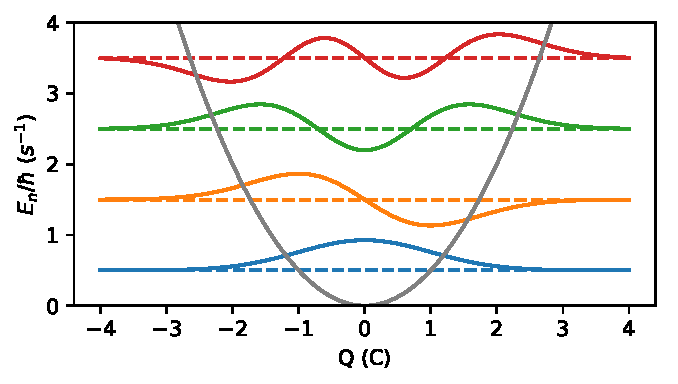
\includegraphics[width=.6\linewidth]{planck_oscillator}
	\caption{Численное решение стационарного уравнения Шредингера для гармонического осциллятора: изображены низшие четыре собственных энергетических уровня (штриховые линии) и состояния гамильтониана (цветные сплошные линии, не в масштабе, за ноль принят соответствующий уровень энергии). Серая сплошная линия показывает потенциальную энергию системы. Параметры $L = 1$ Гн, $ C = 1$ Ф дают циклическую частоту перехода в 1 рад/c.}
	\label{fig:planck_oscillator}
	% построено с помощью Finite difference eigensolver в папке /home/gleb/Projects/Examples/
\end{figure}


Идентичный результат был бы получен при использовании потокового базиса. Однако интересно также рассмотреть энергетический базис, в котором оператор Гамильтона будет диагональным. Для перехода в него будет использоваться так называемое ``вторичное квантование'', использующее операторы рождения и уничтожения фотонов в осцилляторе $\hat a^\dag$ и $\hat a$, $[\hat a, \hat a^\dag] = 1$. Произведением замены 
\begin{align}
	\hat Q \rightarrow \sqrt{\frac{\hbar \omega_r C}{2}}(\hat a^\dag + \hat a),\\
	\hat \Phi \rightarrow i\sqrt{\frac{\hbar \omega_r L}{2}}(\hat a^\dag - \hat a)
\end{align}
гамильтониан приводится к диагональному виду:
\begin{equation}
	\hat{\mathcal H} =  \hbar \omega_r (\hat a^\dag \hat a + 1/2).
\end{equation}

Ненулевая энергия флуктуаций заряда в основном состоянии оказывается проблемой в случае квантования электромагнитного излучения в вакууме: свободное излучение после преобразования Фурье может представляется квантовомеханически как набор квантовых осцилляторов с непрерывным спектром всевозможных частот. Если учесть, что в основном состоянии энергия каждого равна $\hbar \omega/2$, интеграл полной энергии флуктуаций вакуума окажется расходящимся. Даже если взять в интеграле некоторую верхнюю отсечку по частоте, как часто делается в квантовой электродинамике, энергия пустого пространства окажется на 120 порядков больше, чем предсказывается космологической постоянной в общей теории относительности; в то же время, гравитационного эффекта, который был бы вызван энергией нулевых флуктуаций, действительно не наблюдается. С другой стороны, действие вакуумных флуктуаций однозначно проявляется в так называемом эффекте Казимира, измеренном сейчас с большой точностью \cite{zou2013casimir}. Подобно ультрафиолетовой катастрофе конца 19 века, эта проблема названа вакуумной катастрофой и до сих пор не разрешена \cite{adler1995vacuum}.

\subsection{Квантование произвольных электрических цепей по Деворе}

На заре экспериментов с макроскопическими квантовыми системами Мишелем Деворе была создана методика для квантования произвольных электрических цепей, которая отразилась в его методичке 1995 года ``Квантовые флуктуации в электрических цепях'' \cite{devoret1995quantum}. По большому счету, в этой работе не содержится ничего, чего не было бы в стандартных аналитической и квантовой механиках, однако есть несколько практических замечаний, которые пригодятся нам в дальнейшем при рассмотрении более сложных электрических цепей, содержащих джозефсоновсие переходы.

Подход Деворе -- квантовать цепи в потоковом базисе, учитывая возможное наличие петель, через которые может проходить внешний магнитный поток. Такой поток оказывается важен, так как его изменение может создавать ЭДС в замкнутом контуре и явно входить во второй закон Кирхгофа. Если работать в потоковом базисе (проинтегрировать все напряжения во втором законе Кирхгофа по времени), такой поток окажется просто включенным в уравнения, и, следовательно, в Лагранжиан. 

Поучительным в данном случае является пример гармонического осциллятора, который формально представляет собой кольцо, в котором можно записать второй закон Кирхгофа. Представим, что в через данное кольцо физически проходит некий поток $\Phi_e$. Тогда в потоковом базисе второй закон Кирхгофа запишется как
\begin{equation}
	-L\dot I_L - Q_C/C = \dot \Phi_e.
\end{equation}
Интегрируя по времени и подставляя в первый закон Кирхгофа, получим:
\begin{equation}
	\Phi_L/L = - (\ddot \Phi_L + \ddot \Phi_e)C.
\end{equation}
Как можно видеть, в случае электрического осциллятора в уравнение движения входит вторая производная от внешнего потока. Таким образом, если он является постоянным или даже линейно меняющимся во времени, никакого эффекта на динамику он не оказывает. В противном же случае его надо учитывать в явном виде.

Посмотрим теперь, как подходит к этой проблеме Деворе. В формуле (2.13) из \cite{devoret1995quantum} мы обнаруживаем, как второй закон Кирхгофа учитывается при определении потоковой переменной на элементе, заканчивающем неустранимый контур. Такой элемент не создает новой степени свободы в системе, а лишь использует старые степени свободы (узловые потоки, см. определение там же \cite{devoret1995quantum}). Для демонстрации подхода несколько усложним контур электрического осциллятора, добавив в него новую индуктивность параллельно или последовательно со старой, см. \autoref{fig:llc}.
\begin{figure}
	\centering
	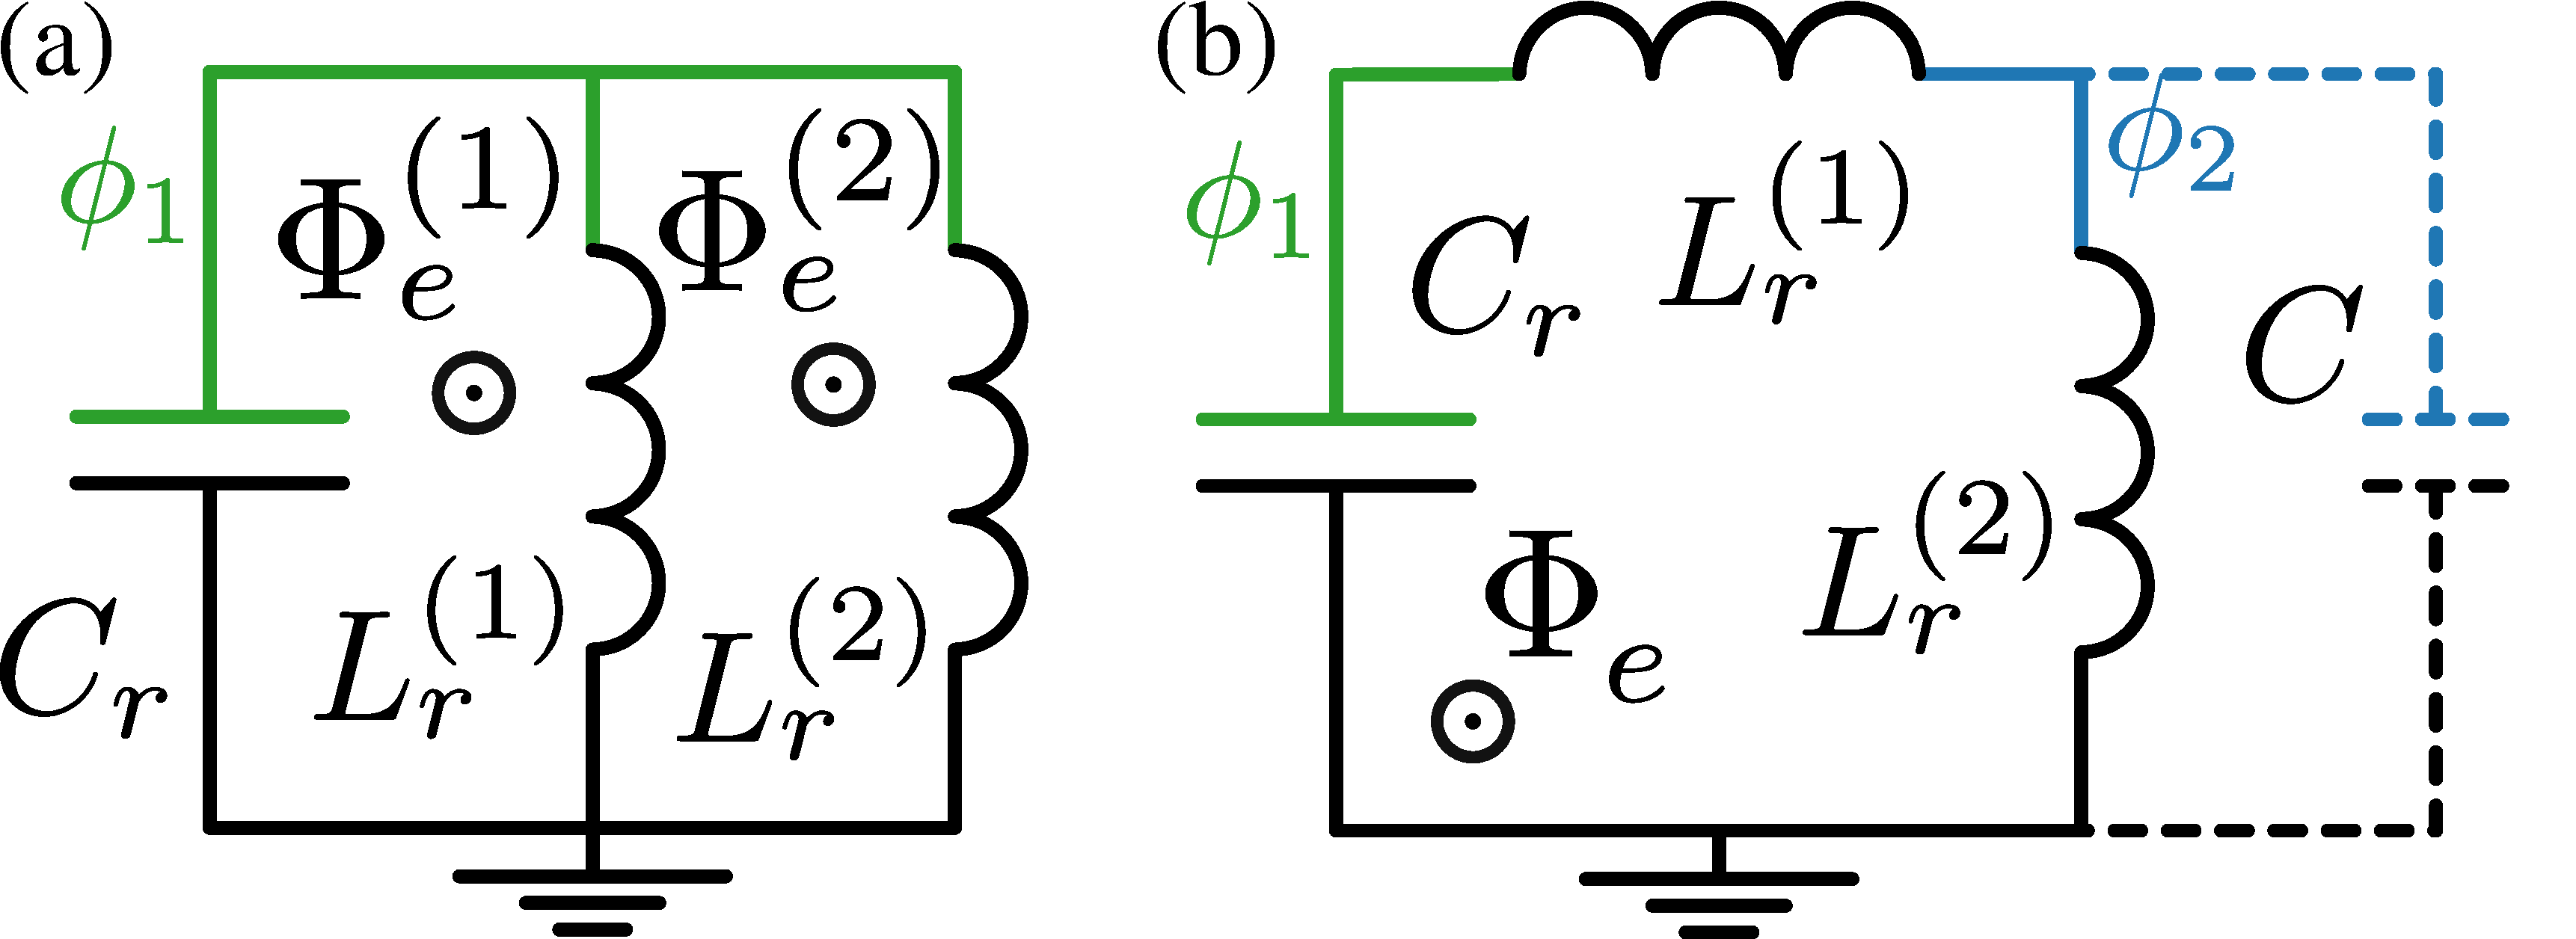
\includegraphics[width=0.8\linewidth]{Pictures/LLC}
	\caption{Две конфигурации осциллятора с добавленными индуктивностями: параллельно \textbf{(a)} и последовательно \textbf{(b)}. Узловые фазовые переменные (степени свободы) обозначены буквами $\phi$ и соответствующим цветом.}
	\label{fig:llc}
\end{figure}

Для параллельного соединения обе индуктивности являются элементами, закрывающими свой контур. Поэтому для катушек мы записываем:
\begin{align}
	\Phi_L^{(1)} &= \phi_1 - 0 + \Phi_e^{(1)},\\
	\Phi_L^{(2)} &= \phi_1 - 0 + \Phi_e^{(2)},
\end{align}
где мы использовали тот факт, что ``земля'' имеет по определению нулевое значение узлового потока. В таком случае лагранжиан в потоковом базисе запишется как 
\begin{equation}
	\mathcal{L}_{L||L||C} = \frac{C_r \dot\phi_1^2}{2} - \frac{\left(\phi_1 + \Phi_e^{(1)}\right)^2}{2L_r^{(1)}} - \frac{\left(\phi_1 + \Phi_e^{(2)}\right)^2}{2 L_r^{(2)}}.
\end{equation}

Как видим, внешние потоки явно входят в лагранжиан, и, очевидно, будут присутствовать и в гамильтониане системы. Однако при ближайшем рассмотрении потенциала выясняется, что его форма остается неизменной параболической для любых конфигураций значений индуктивностей и потоков сквозь петли; единственным эффектом внешних потоков является постоянное смещение минимума потенциальной энергии относительно параметра $\phi_1$. Колебания же будут определяться квадратичным членом с эффективной индуктивностью $L_r = L_r^1 || L_r^2$ параллельно соединенных катушек. Тот же результат мы получили бы, если бы заранее объединили катушки согласно правилу сложения индуктивностей и применяли процедуру к уже упрощенному контуру (предварительное упрощение часто применяется для сложных цепей, см., например, \cite{koch2007charge}). 

Рассмотрим теперь последовательное соединение катушек, \autoref{fig:llc}~(b) (без штрихованного конденсатора). В отличие от предыдущего случая, мы обнаруживаем, что число степеней свободы увеличилось с добавлением новой индуктивности, а единственный контур сохранился. Лагранжиан такой системы:
\begin{equation}
	\mathcal{L}_{LL||C} = \frac{C_r \dot\phi_1^2}{2} - \frac{(\phi_2 - \phi_1)^2}{2L_r^{(1)}} - \frac{\left(\phi_2+\Phi_e\right)^2}{2 L_r^{(2)}}.\label{eq:ll||c}
\end{equation}

Из вида лагранжиана становится очевидно, что переменная $\phi_2$ оказывается зависимой. Действительно, уравнение Лагранжа-Эйлера на нее запишется следующим образом:
\begin{equation}
	\phi_2/L_r^{(1)} + \phi_2/L_r^{(2)} + \Phi_e/2L_r^{(2)} = \phi_1/L_r^{(1)}.
\end{equation}
Подставляя выраженное отсюда $\phi_2$ в оставшееся уравнение Эйлера-Лагранжа, мы получим уравнение колебаний на $\phi_1$ с эффективной индуктивностью $L_r^{(1)} + L_r^{(2)}$. Очевидно, именно так и должно было получиться, если бы мы опять применили правило сложения теперь уже последовательных индуктивностей. Магнитный поток, конечно, также войдет в уравнения движения, но не будет влиять на динамику системы при условии независимости его от времени. 

Но каковы же будут решения уравнения Шредингера, составленного с использованием лагранжиана \eqref{eq:ll||c}? Из-за отсутствия обобщенного импульса по $\phi_2$ ($\partial \mathcal{L}_{LL||C}/\partial \dot \phi_2 = 0$) в операторе Гамильтона не будет второй производной по этой координате. Это приведет к тому, что собственные функции в направлении $\phi_2$ окажутся дельта-функциями и суперпозициями дельта-функций. Также это будет означать, что в силу соотношения неопределенностей узловой заряд $q_2$ на острове, отмеченном синим на \autoref{fig:llc}~(b), окажется полностью делокализованным, так как является канонически сопряженным бесконечно локализованному дельта-функцией узловому потоку $\phi_2$. Численное решение такого уравнения Шрёдингера оказывается невозможным, так как спектр задачи является непрерывным и не может быть воспроизведен диагонализацией конечномерных матриц. Результаты такого наивного решения приведены на \autoref{fig:llcstatesdelta}~(a). Как можно видеть, алгоритм воспроизводит дискретные дельта-функции по оси $\phi_2$ и правильно определяет структуру собственного состояния гармонического осциллятора по оси $\phi_1$, однако рассчитанный энергетический спектр системы оказывается в целом неверным. Физически полная делокализация узлового заряда также невозможна, так как означала бы ненулевую вероятность обнаружения произвольно большого заряда на соответствующем острове. 

\begin{figure}
	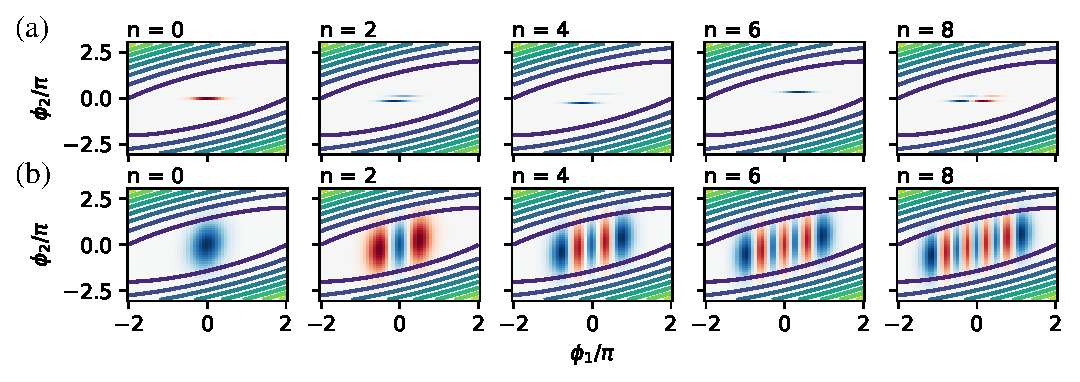
\includegraphics[width=\linewidth]{Pictures/llc_states}
	\caption{Собственные состояния модели \autoref{fig:llc}~(b) при $C = 0$ \textbf{(a)} и $C = C_r/100$ \textbf{(b)} (показаны чётные номера). В обоих случаях $C_r = 1, L_r^{(1)} = L_r^{(2)} = 0.5$. При $C = 0$ численные собственные значения зависят от шага сетки и оказываются неверными. В другом случае же ответ получается верным: спектр эквидистантный с шагом $\omega_r \approx 1\ \text{s}^{-1}$. Контурными линиями показана потенциальная энергия из \eqref{eq:ll||c}. В каждом направлении пространство разбито на 50 ячеек.}
	\label{fig:llcstatesdelta}
	% построено с помощью Finite difference eigensolver в папке /home/gleb/Projects/Examples/
\end{figure}

Как видим, в классическом случае схема \autoref{fig:llc}~(b) без штрихованного конденсатора допускает физически осмысленное решение. Однако в квантовом случае для получения осмысленного результата требуется учитывать малый конденсатор $C$ для освобождения потоковой переменной $\phi_2$ (для простоты будем считать, что в новом кольце поток равен нулю). На практике такая емкость всегда будет существовать из-за конечных размеров проводника, отмеченного синим цветом. Интересно также, что переход от локализации к делокализации $\phi_2$ происходит скачком при непрерывном уменьшении емкости конденсатора до нуля. Пример состояний, получающихся при правильной диагонализации изображен на \autoref{fig:llcstatesdelta}~(b). Как видим, структура волновой функции в направлении $\phi_2$ предполагает основное состояние нового дополнительного осциллятора. 

Для полноты картины требуется также определить, какая структура колебаний будет у классической модели с дополнительным конденсатором. При добавлении новой степени свободы для нахождения нормальных мод колебаний потребуется решить вековое уравнение:
\begin{equation}
	\text{det}(\Pi - \lambda T) = 0,
\end{equation}
где $T$ -- квадратичная форма потенциальной энергии, а $\Pi$ -- квадратичная форма кинетической энергии системы. Лагранжиан с учётом добавленной емкости:
\begin{equation}
\mathcal{L}_{LL||C+C} = \frac{C_r \dot\phi_1^2}{2} + \frac{C \dot\phi_2^2}{2} - \frac{(\phi_2 - \phi_1)^2}{2L_r^{(1)}} - \frac{\phi_2^2}{2 L_r^{(2)}}.
\end{equation}
Используя модифицированный лагранжиан, получаем следующие выражения:
\begin{equation}
	\Pi = \left(
	\begin{matrix}
	\frac{1}{L_r^{(1)}}&-\frac{1}{L_r^{(1)}}\\
	-\frac{1}{L_r^{(1)}}&\frac{L_r^{(1)}+L_r^{(2)}}{L_r^{(1)}L_r^{(2)}}
	\end{matrix}\right),\ 
	T = \left(
	\begin{matrix}
	C_r& 0 \\
	0 & C
	\end{matrix}\right).
\end{equation}
Разложение в ряд Тейлора решений векового уравнения вблизи $C = 0$ дает два решения:
\begin{equation}
	\lambda_{1,2} = \frac{1}{C_r\left(L_r^{(1)}+L_r^{(2)}\right)},\quad \frac{L_r^{(1)}+L_r^{(2)}}{C L_r^{(1)}L_r^{(2)}}.
\end{equation}
Видно, что колебания дополнительного осциллятора в случае малой емкости его острова происходят на очень высокой частоте $\sqrt{\lambda_2}$. На языке импедансов можно сказать, что реактивное сопротивление большого конденсатора $C_r$ в этом режиме стремится к нулю, и он может быть заменен закороткой. Тогда сразу становится понятна и форма ответа для частоты колебаний побочного осциллятора: эффективная индуктивность складывается из параллельно подключенных $L_r^{(1)}$ и $L_r^{(2)}$. Таким образом, мы определили, как корректно работать с последовательно подключаемыми индуктивностями и в квантовом случае, и в классическом.

\begin{figure}
	\centering
	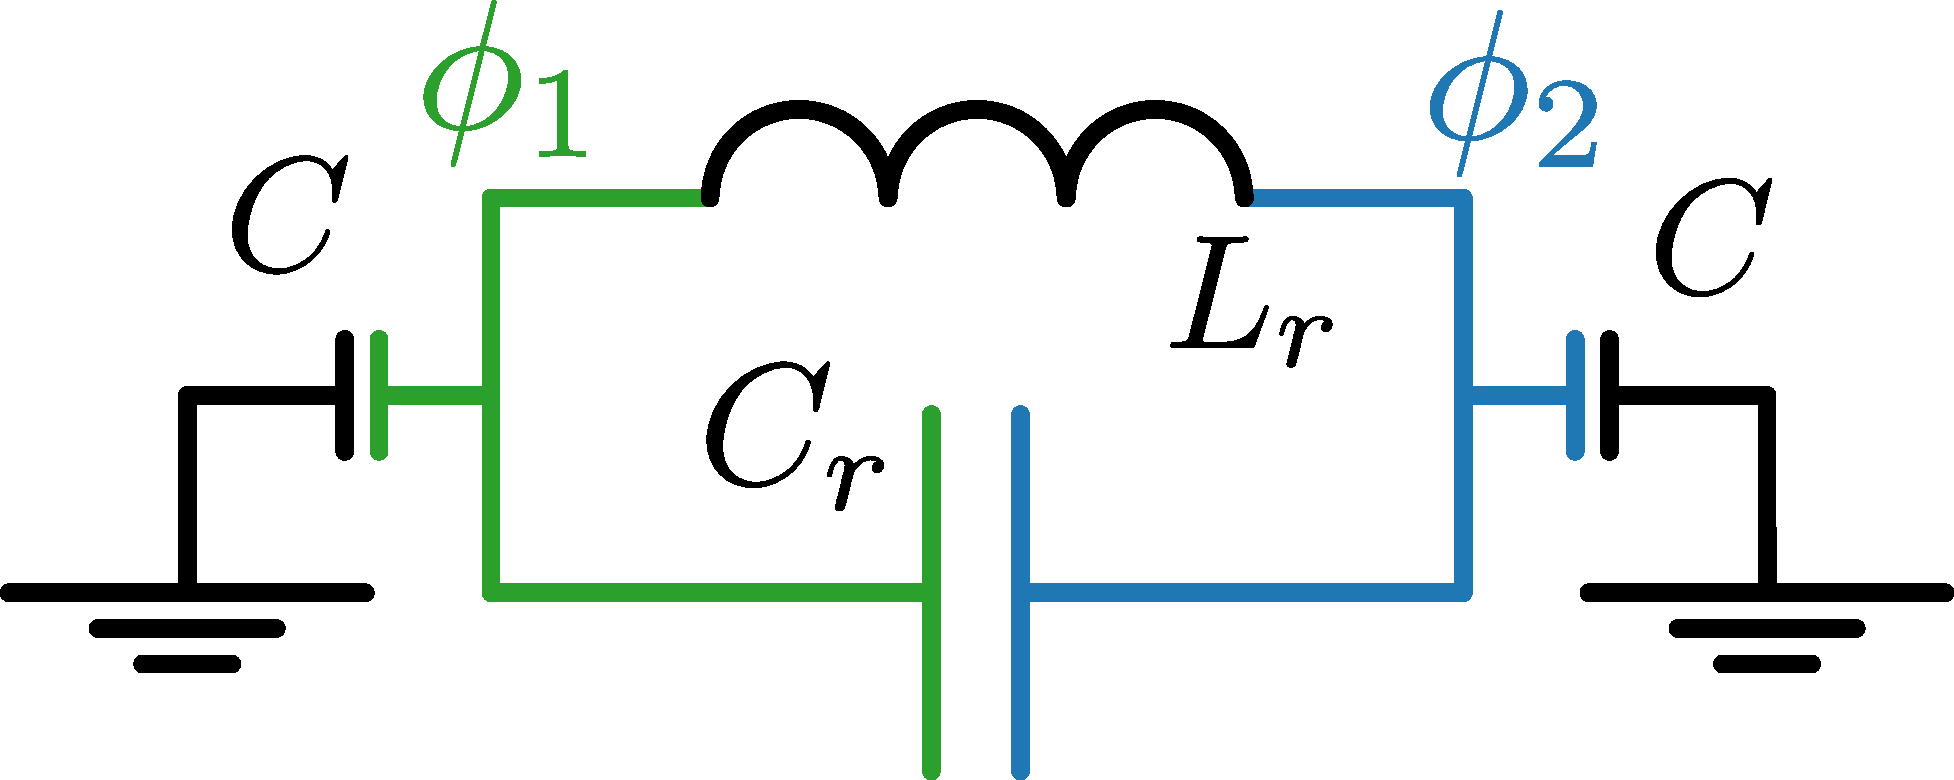
\includegraphics[width=0.5\linewidth]{Pictures/lc_cap_inv}
	\caption{Осциллятор, заземленный через конденсаторы малой ёмкости.}
	\label{fig:lccapinv}
\end{figure}

Добавление малых емкостей на землю параллельно уже существующим большим конденсаторам может привести к подобным проблемам в случае решения задач в зарядовом базисе. Рассмотрим пример такой проблемы для еще одной электрической схемы, изображенной на \autoref{fig:lccapinv}. Лагранжиан системы запишется как
\begin{equation}
	\mathcal{L}_{LCg} = \frac{C \dot \phi_1^2}{2} + \frac{C \dot \phi_2^2}{2} + \frac{C_r\left(\dot\phi_1 - \dot\phi_2\right)^2}{2} - \frac{L_r \left(\phi_1  - \phi_2\right)^2}{2}.\label{eq:l_lcg}
\end{equation}
Как видим, квадратичная форма кинетической энергии (коэффициенты её также называются матрицей ёмкостей) здесь не приведена к диагональному виду. Поэтому чтобы получить гамильтониан через преобразование Лежандра, потребуется решить систему линейных уравнений на $\phi_{1,2}$ относительно $q_{1,2}$. После этого гамильтониан запишется как 
\begin{equation}
	\mathcal{H}_{LCg} = \frac{1}{2} \left(\begin{matrix} q_1\\q_2\end{matrix}\right) \left(\begin{matrix}
	C+C_r & -C_r \\
	-C_r & C+C_r
	\end{matrix}\right)^{-1}\left(\begin{matrix} q_1&q_2\end{matrix}\right)+\frac{L_r \left(\phi_1  - \phi_2\right)^2}{2}.
\end{equation}
Проблема здесь заключается главным образом в том, что потенциальная энергия не имеет роста по направлению $\phi_1 + \phi_2$, и волновые функции окажутся делокализованными. Очевидно, что такая проблема не возникла бы, если бы мы изначально исключили энергии малых конденсаторов из лагранжиана и осуществили бы замену координат $\phi_1 - \phi_2 \rightarrow \phi$, уменьшив реальное число степеней свободы. Проанализируем, насколько эта ситуация сходна с предыдущей.

Для начала попробуем решить вековое уравнение, задаваемое \eqref{eq:l_lcg}. Его решениями окажутся
\begin{equation}
	\lambda_{1,2} = 0,\ \frac {1}{L_r \left( C/2 + C_r \right) }.	
\end{equation}
Нулевое решение сразу говорит нам о том, что система может существовать в состоянии безразличного равновесия когда $\phi_1 = \phi_2$. Физически это означает, что потенциалы на островах равны во все моменты времени, а заряды их, соответственно, должны быть какими угодно, но одинаковыми. Ненулевое решение отвечает осцилляциям, в которых малые конденсаторы складываются последовательно друг с другом, а затем параллельно с конденсатором $C_r$. Выражение легко понять, если вместо соединения конденсаторов $C$ землей соединить их друг с другом, а землю вообще исключить из схемы. В целом мы видим, что классическое решение, основанное на вековом уравнении, не встречает трудностей с такой системой.

Решение уравнения Шрёдингера численно методом конечных разностей в такой постановке невозможно. Частица в заданном потенциале будет иметь непрерывный энергетический спектр, для которого, как уже обсуждалось ранее, дискретизовать задачу в принципе нельзя. Поэтому для успешного численного решения в подобных ситуациях требуется сначала провести аналитическую замену координат:
\begin{equation}
	\begin{aligned}
		\phi_1 &= \frac{\phi_+ + \phi_-}{2},\\
		\phi_2 &= \frac{\phi_+ - \phi_-}{2}.
	\end{aligned}
\end{equation}
Тогда лагранжиан запишется в виде
\begin{equation}
	\mathcal{L}_{LCg} = \frac{(C_r+C/2)\dot\phi_-^2}{2}  + \frac{C \dot\phi_+^2}{4} - \frac{L_r \phi_-^2}{2}.
\end{equation}
Фактически, был произведен переход к нормальным координатам, и уравнения на степени свободы разделились. Нахождение обратной матрицы емкости теперь не представляет трудности, и гамильтониан запишется как 
\begin{equation}
	\mathcal{H}_{LCg} = \frac{q_-^2}{2(C_r+C/2)} + \frac{q_+^2}{C} + \frac{L_r \phi_-^2}{2}.
\end{equation}
Переходя к операторному виду, будем искать решения уравнения Шрёдингера в виде $\psi(\phi_+, \phi_-) = \psi_+(\phi_+)\psi_-(\phi_-)$, a общую энергию в виде $E = E_1+E_2$. После разделения переменных по методу Фурье, получим два уравнения
\begin{equation}
	\begin{aligned}
	-\frac{\hbar^2}{C}\frac{\partial^2}{\partial \phi_+^2}\psi_+ - E_1\psi_+ &= - \lambda\psi_+,\\
	-\frac{\hbar^2}{2(C_r + C/2)}\frac{\partial^2}{\partial \phi_-^2}\psi_- + \frac{L_r \phi_+^2}{2}\psi_- - E_2\psi_+ &= \lambda\psi_-.
	\end{aligned}
\end{equation}
Обозначая собственные энергии как $E^+ = E_1 - \lambda,\ E_n^- = E_2 + \lambda$, получим для исходных энергий $E = E^+ + E_n^-$. Первое уравнение решается аналитически и дает непрерывный спектр, второе же воспроизводит задачу для одномерного гармонического осциллятора с эффективной емкостью $C_r+C/2$. Таким образом, после замены разделения переменных решение задачи численно становится возможным. 

В заключение обозначим дуализм между двумя проблемными случаями, описанными выше. В первом случае дополнительная степень свободы не давала вклад в кинетическую энергию системы, а во втором случае -- в потенциальную. С учетом того, что роль кинетической и потенциальной энергии выбирается при выборе обобщенных координаты и импульса, разницы между двумя этими ситуациями на самом деле нет. В обоих случаях проблемы с численным решением были вызваны непрерывностью спектра системы. Однако в первом случае, в отличие от второго, нельзя разделить переменные в уравнения Шрёдингера и получить аналитическое решение для степени свободы с непрерывным спектром. Поэтому для успешного численного решения необходимо ввести дополнительный элемент, локализующий заряд на острове. Точно также можно было бы ввести большие по величине индуктивности во втором примере параллельно с малыми конденсаторами для локализации узлового потока. Локализация и делокализация связаны с известным свойством преобразования Фурье:
\begin{equation}
	2\pi\, \delta(\phi) = \int\limits_{-\infty}^{\infty} e^{iq\phi} \diff q,
\end{equation}
и тем фактом, что волновые функции в представлениях канонически сопряженных переменных являются Фурье-образами друг друга. В дальнейшем мы еще затронем тему квантования сверхпроводниковых цепей, так как джозефсоновские переходы вносят в неё свою специфику, связанную с дискретностью узловых зарядов.

\subsection{Учет внешнего возмущения}\label{sec:driven_lc}


\begin{figure}[b]
	\centering
	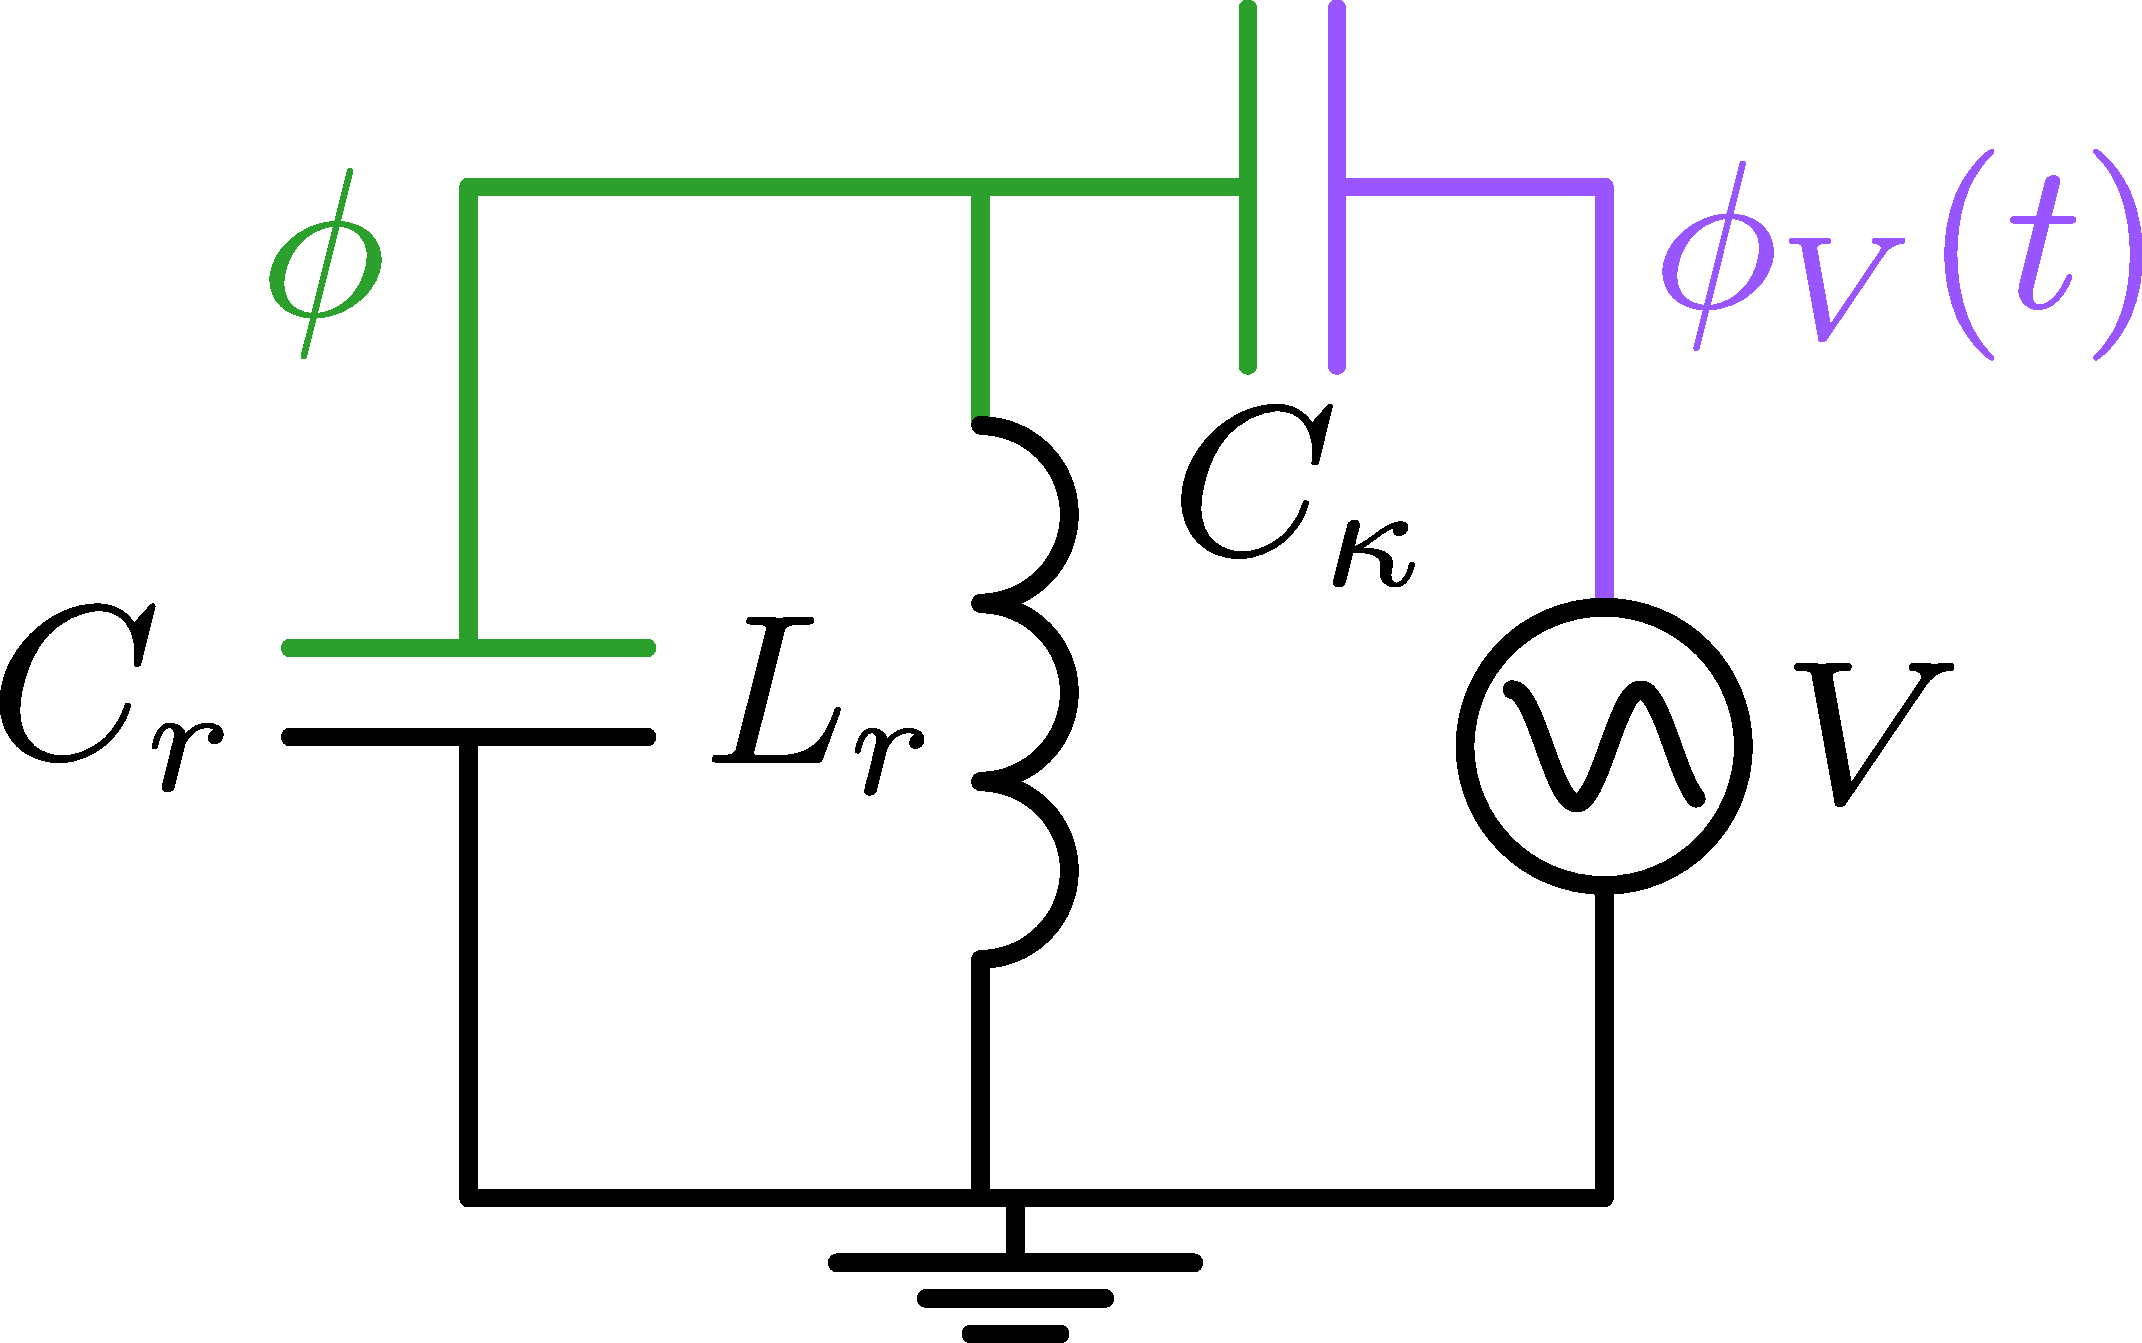
\includegraphics[width=0.4\linewidth]{Pictures/LC_driven}
	\caption{Схема осциллятора со степенью свободы $\phi$, подсоединенного к источнику напряжения $V$ через конденсатор $C_\kappa$. Узловой поток на фиолетовой ветке считается заданным граничным условием, так как влияние колебательного контура на параметры выходного сигнала источника принимается пренебрежимо малым.}
	\label{fig:lcdriven}
\end{figure}

Изолированные электрические цепи представляют малый практический интерес, так как в эксперименте они обязательно подключаются к внешним измерительным приборам: с их стороны цепь подвергается воздействию постоянных или переменных напряжений. Здесь с точки зрения теоретической механики кратко рассмотрим правила учета второго типа воздействия. Рассмотрим схему, изображенную на \autoref{fig:lcdriven}. Главной идеей, которая позволяет составить правильный лагранжиан для системы является предположение о том, что осциллятор не может оказывать серьезного влияния на источник напряжения. Здесь можно представить механическую аналогию -- два маятника с одинаковым периодом колебаний, связанные пружиной. Если у одного из маятников масса груза будет во много раз больше массы груза другого, то колебания его не будут существенно отличаться от свободных. Точно таким же образом в цепи, изображенной на \autoref{fig:lcdriven}, степень свободы, связанная с источником напряжения, будет зависеть от времени так же, как если бы подключения осциллятора не было вовсе (масса здесь заменяется емкостью). Зная это, легко написать лагранжиан, рассчитывая энергию связывающего конденсатора обычным способом:
\begin{equation}
	\mathcal{L}_{{LCdr}} =\frac{C_r \dot\phi^2}{2} - \frac{\phi^2}{2L} + \frac{C_\kappa (\dot\phi - \dot\phi_V(t))^2}{2}.
\end{equation} 
Как видно, эффективная емкость осциллятора после преобразований окажется равной $C_r + C_\kappa$, а уравнения движения на $\phi$ не изменятся, если отбросить квадратичный по узловому потоку источника член. Для составления гамильтониана требуется в явном виде рассмотреть источник как $LC$-контур с большой емкостью, чтобы полная система была консервативной. Тогда из обратной матрицы емкости для этой системы можно при емкости источника $C_V \gg C_r, C_\kappa$ приближенно вычислить коэффициент взаимодействия, содержащий первую степень $q$ -- сопряженного к $\phi$ узлового заряда:
\begin{equation}
	\mathcal{H}_{int} = \frac{C_\kappa}{C_\kappa + C_r} \frac{q q_V}{C_V},
\end{equation}
где использовано обозначение $q_V = C_V \dot\phi_V(t)$. Далее осуществляется переход к операторному виду по стандартному методу и решение нестационарного уравнения Шредингера для расчета динамики квантового состояния под действием излучения.


\section{Сверхпроводимость и эффект Джозефсона}

\subsection{Теория Лондонов}

Сверхпроводимость была экспериментально обнаружена в 1911 году голландским ученым Хейке Камерлинг-Оннесом в ртути при гелиевых температурах. Именно он также впервые получил и жидкий гелий, без которого невозможно было бы получить необходимую низкую температуру, за что уже через два года был удостоен Нобелевской премии. Открытие это было скорее случайным, так как никто до этого даже и представить не мог возможность такого эффекта, не то что предсказать его. Впоследствии достаточно долго считалось, что явление заключается лишь в падении до нуля электрического сопротивления металлов, и только в 1933 году немцами Вальтером Мейсснером и Робертом Оксенфельдом был обнаружен эффект абсолютного диамагнетизма сверхпроводников. 

Первым шагом к пониманию природы сверхпроводимости стала феноменологическая теория немецких физиков Фрица и Хайнца Лондонов \cite{london1935electromagnetic}. Рассуждение авторов начинается с ``уравнения ускорения'', которое было принято в то время для описания ``сверхпроводящих'' электронов, движущихся без трения:
\begin{equation}
	\Lambda \dot{\mathbf{J}} = \mathbf{E},\ \Lambda = m/ne^2. \label{eq:acceleration}
\end{equation}
Здесь $m$ -- это масса сверхпроводящих электронов, $e$ -- их заряд, $n$ -- концентрация. Если взять ротор от этого уравнения, учесть третье уравнение Максвелла и тот факт, что дивергенция магнитного поля равна нулю, а затем проинтегрировать по времени, то можно получить следующее равенство:
\begin{equation}
	\Lambda c^2 \nabla^2 (\mathbf{H}-\mathbf{H}_0) = \mathbf{H} - \mathbf{H}_0,\label{eq:london_inhomogeneous}
\end{equation}
где $\mathbf{H_0}$ -- это значение напряжённости магнитного поля в некий нулевой момент времени. Физически осмысленные решения однородного уравнения при $\mathbf{H_0} = 0$ оказываются экспоненциально спадающими при углублении в толщу сверхпроводника, а частное решение $\mathbf{H} = \mathbf{H}_0$ таким образом предсказывает возможность ``вмораживания'' начального магнитного поля в сверхпроводник после перехода его в сверхпроводящее состояние. Однако эксперимент Мейсснера опровергает подобный вывод: достаточно слабое магнитное поле выталкивается из сверхпроводника при переходе через критическую температуру. Это и отличает гипотетический идеальный проводник, описываемый уравнением \eqref{eq:acceleration}, от реальных сверхпроводников.

Так как уравнение \eqref{eq:london_inhomogeneous} правильно описывает затухающее внутри сверхпроводника магнитное поле в однородном случае, Лондоны предложили постулировать $\mathbf{H_0} = 0$ и преобразовать однородное уравнение обратно к виду
\begin{equation}
	\nabla \times \Lambda \mathbf J = -\frac{1}{c} \mathbf{H},\label{eq:london_first}
\end{equation}
фактически опуская дифференцирование по времени и константу интегрирования, возникавшую в прямом преобразовании. Данное уравнение уже не приводит к уравнению \eqref{eq:acceleration}. Вместо него может быть получено более слабое утверждение
\begin{equation}
	\nabla \times (\Lambda \dot{\mathbf J} - \mathbf E)  = 0,
\end{equation}
или, что то же самое,
\begin{equation}
	 \Lambda \dot{\mathbf J} - \mathbf E = \nabla \mu. \label{eq:london_second}
\end{equation}
Для соблюдения Лоренц-инвариантности можно выбрать $\mu = -\Lambda c^2 \rho$, $\rho = \nabla\cdot\mathbf E$, и тогда выводится еще одно уравнение:
\begin{equation}
	\Lambda (\dot{\mathbf J} + c^2 \nabla \rho) = \mathbf E.
\end{equation}
Отсюда следует, что 
\begin{gather}
	\Lambda c^2 \nabla^2 \mathbf E = \mathbf E,\\
	\Lambda c^2 \nabla^2 \rho = \rho.
\end{gather}
Такие уравнения предполагают, что статическое электрическое поле проникает в сверхпроводник так же, как и статическое магнитное, экспоненциально затухая на глубине $d = \sqrt{\Lambda c^2}$. Однако, как вскоре выяснилось, такой выбор $\mu$ для соблюдения Лоренц-инвариантности является неверным. Чтобы проверить, действительно ли электрическое поле проникает внутрь сверхпроводника, через несколько месяцев после вышеописанной работы Хайнц Лондон провел эксперимент с ртутным конденсатором \cite{london1936experimental}. В случае, если проникновение поля в сверхпроводящей фазе имело бы место, то емкость такого конденсатора при сверхпроводящем переходе уменьшилась бы на величину порядка $2d$ из-за эффективного удаления обкладок друг от друга. Однако такого эффекта с большой точностью в эксперименте обнаружено не было. Таким образом, статическое электрическое поле в сверхпроводнике существовать не может так же, как и в нормальном металле\footnote{Интересно отметить, что и до сей поры в авторитетных изданиях продолжают выходить публикации, спорящие с этим. Они утверждают, что статическое электрическое поле в сверхпроводник всё-таки проникает, причем на основе этого эффекта можно даже создать полевой транзистор \cite{de2018metallic, paolucci2018ultra}. Альтернативное объяснение наблюдаемым в указанных работах эффектам можно найти в работе \cite{golokolenov2020origin}.}. Поэтому  правильным выбором калибровки будет $\mu=0$, что возвращает нас к исходному уравнению ускорения \eqref{eq:acceleration}. Подводя итог, запишем правильные уравнения Лондонов современном виде как
\begin{align}
\Lambda c\, \nabla \times \mathbf J &= - \mathbf H,\\
\Lambda \dot{\mathbf J} &= \mathbf E.
\end{align}

\subsection{Теория Пиппарда}

В последующие годы эксперименты со статическим магнитными и электрическими полями в рамках исследования свойств сверхпроводников перетекли к опытам с переменным током. По аналогии с аномальным скин-эффектом в чистых металлах, где длина свободного пробега электронов оказывается сравнима с толщиной скин-слоя, в 1953 году англичанин Брайан Пиппард предложил обобщение эмпирических уравнений Лондонов нелокальным интегральным уравнением \cite{pippard1953experimental}. Исток этой идеи заключается в эксперименте, проведенным автором в той же работе: исследовалась глубина проникновения магнитного поля в олово в зависимости от концентрации примеси индия\footnote{Глубина проникновения измерялась косвенно по изменению частоты сверхпроводящего резонатора при превышении критического магнитного поля \cite{pippard1950surface}.}. Оказалось, что при изменении концентрации индия от 0  до 3\% глубина проникновения магнитного поля менялась практически в два раза, хотя критические температура и магнитное поле менялись несущественно. В то же время, сопротивление загрязненного олова оказывается в 1200 раз выше, а длина свободного пробега в нем электронов во столько же раз ниже. Таким образом, Пиппардом была открыта некая пока необъяснимая связь между длиной свободного пробега электронов в нормальном состоянии и глубиной проникновения магнитного поля в сверхпроводник.

К нелокальному уравнению автор пришел, преобразуя сперва \eqref{eq:london_first} к виду 
\begin{equation}
	\Lambda \mathbf J + \mathbf A = 0,
\end{equation}
где $\mathbf A$ -- это векторный потенциал с правильной калибровкой. Далее Пиппард вводит некую длину $\xi$ в сверхпроводнике по аналогии с длиной свободного пробега, которая фигурирует в законе, напоминающем закон Ома для обычных проводников:
\begin{equation}
	\mathbf J = - \frac{\xi}{\xi_0 \Lambda} \mathbf A.
\end{equation}
Далее постулируется интегральное уравнение:
\begin{equation}
	\mathbf J = - \frac{3}{4\pi \xi_0 \Lambda} \int \mathbf r \frac{ \mathbf r\cdot \mathbf A\, e^{-r/\xi}}{r^4} \diff^3 r.
\end{equation}
Из этого уравнения Пиппардом было получено аналитическое выражение для глубины проникновения (см. формулу (12) из \cite{pippard1953experimental}) в зависимости от введенной постоянной $\xi$. Оказалось, что глубина проникновения в случае $\xi \ll \lambda$ ведет себя как $1/\sqrt{\xi}$, а в противном случае не зависит от $\xi$. Хорошее совпадение с экспериментальными данными дает выражение, связывающее $\xi$ с длиной свободного пробега простым законом пропорциональности (коэффициент определялся в статье методом аппроксимации), однако получить правильное значение для $\xi_0$ -- предела $\xi$ для чистого олова при нулевой температуре -- из такого закона Пиппарду не удалось.

\subsection{Теория БКШ}

Спустя всего 4 года после работы Пиппарда вышла статья американцев Джона Бардина, Леона Купера и Джона Шриффера \cite{bardeen1957theory}, удостоенная впоследствии Нобелевской премии 1972 года, которая построила полностью квантовомеханическую модель для так называемых обычных сверхпроводников. Конечно, эта теория родилась не на пустом месте и была в значительное мере предопределена развитием квантовой теории металлов. Еще в 1937 году Слэтер \cite{slater1937nature} размышлял о природе сверхпроводящего состояния в одноименной работе и предполагал, что теория возмущений, примененная к стандартным блоховским функциям электронов, может породить некоторое ``особенное состояние'', отделенное от основного непрерывного спектра частично заполненной зоны проводника. Отделение приведет к тому, что локальная плотность состояний, видимая электроном, уменьшится практически до нуля, что в стандартной блоховской теории означает отсутствие сопротивления вследствие малой вероятности рассеяния. Помимо этого в 1938 году независимо Петром Капицей \cite{kapitza1938viscosity} (турбулентный случай) и Джоном Алленом и Доном Мизенером \cite{allen1938flow} (ламинарный случай) была окончательно установлена сверхтекучесть гелия-4, а Фриц Лондон предположил, что явление объясняется Бозе-Эйнштейновской конденсацией \cite{london1938lambda}. Явления сверхтекучести и сверхпроводимости были очевидно связаны друг с другом и требовали общего объяснения.

Предвестниками работы БКШ были и достаточно лаконичная работа Бардина \cite{bardeen1955theory}, посвященная вопросу достаточности наличия энергетической щели для объяснения диамагнетизма сверхпроводников, и работа Купера касательно теоретического обоснования существовании энергетической щели в Ферми-газе при введении сколь угодно малого взаимодействия между электронами \cite{cooper1956bound}. Однако, наверное, важнейшим экспериментальным открытием, подтолкнувшего научное сообщество к подробной разработке идеи об электрон-фононном взаимодействии, стал изотоп-эффект \cite{maxwell1950isotope,reynolds1950superconductivity,de1954isotope}, обнаруженный в 1950 году. Оказалось, что различные изотопы ртути имеют разные температуры сверхпроводящего перехода, причем чем меньше масса ядер, тем больше критическая температура. Как раз тогда же, в начале 1950-х годов, Бардин и Герберт Фрёлих практически одновременно друг с другом развивали теорию взаимодействия электронной и фононной подсистем; описание двух теорий можно найти в работе \cite{bardeen1951electron} (стоит отметить, что Фрёлих также пытался объяснить сверхтекучесть в конце 30-х годов). Однако первоначальный подход, опиравшийся главным образом на идею модификации собственных энергий электронов, встретился с трудностями, которые не позволяли назвать эти теории успешными \cite{bardeen1957theory}. Только после точного описания электрон-фононного взаимодействия с учетом электрического экранирования \cite{bardeen1955electron} удалось построить действительно непротиворечивую модель сверхпроводимости, которая используется и по сей день.

В данной работе мы будем пользоваться лишь основными выводами из теории БКШ: наличие общей волновой функции основного состояния куперовских пар с фазой $\phi$. Если фаза зависит от трехмерных координат, то наблюдается течение сверхтока. В этом контексте также можно упомянуть и феноменологическую теорию Льва Ландау и Виталия Гинзбурга, созданную в начале 1950-х годов. Коэффициенты теории вычисляются из теории БКШ \cite{gor1959microscopic}.

\subsection{Эффект Джозефсона}

В 1962 году британский физик Брайан Джозефсон опубликовал работу, предсказывающую два необычных эффекта в связанных сверхпроводниках: первый эффект заключается в том, что при достаточно малом расстоянии между сверхпроводниками через зазор может течь сверхток, а при конечном напряжении на зазоре кроме постоянного сверхтока должен протекать еще и переменный сверхток с частотой, пропорциональной этому напряжению \cite{josephson1962possible}. Вывод в оригинальной работе не слишком изощрен и базируется на модельном гамильтониане
\begin{equation}
	H = \sum_k n_k E_k + \mu_l N_l + \mu_r N_r + \sum_{l,r} T_{lr}a^\dag_l a_r + T_{rl} a^\dag_r a_l, \label{eq:josephson_tunnel}
\end{equation}
где $n_k$ -- число квазичастиц в сверхпроводниках, $\mu_{l,r}$ -- химические потенциалы, определяемые электрическими напряжениями на них $N_{r,l}$ -- числа электронов справа и слева от барьера. Последняя же часть описывает предполагаемое туннелирование электронов со скоростями $T_{lr}$. 

Исторически этот подход опирается на экспериментальные статьи, исследовавшие туннелирование электронов сквозь тонкие диэлектрические барьеры, разделяющие электроды из нормального металла. Например, в работе Дж. К. Фишера и Айвара Джайевера 1960 года  \cite{fisher1961tunneling} измерялось сопротивление тонких оксидных барьеров на алюминии при комнатной температуре. Толщина барьера измерялась по величине электрической емкости между электродами принимая $\epsilon_{Al_2O_3} = 8$. Экспоненциальная зависимость тока от напряжения позволила установить факт туннелирования сквозь барьер при небольших напряжениях порядка 1 В (теоретическая модель туннелирования еще в 1951 году была построена Рагнаром Холмом \cite{holm1951electric}). За год до этого Джайевером измерялись и вольт-амперные характеристики переходов сверхпроводник-изолятор-сверхпроводник \cite{giaever1960energy, giaever1960electron}, однако сверхтока он не обнаружил из-за недостаточной фильтрации сигналов. Еще раньше, начиная с 1958 года, Ганс Мейсснер исследовал сопротивление контактов металл-сверхпроводник \cite{meissner1958measurements, meissner1960superconductivity}, которое уменьшалось до нуля при достаточно малых толщинах нормального электрода. Это позволило сделать вывод о том, что плотность ``сверхпроводящих'' электронов падает в металлическом барьере плавно, а не исчезает сразу же, а значит, возможно и их квантовое туннелирование.

Непосредственно предшествующей статье Джозефсона была работа Моррела Кохена, Леопольдо Фаликова и Джеймса Филлипса 1962 года \cite{cohen1962superconductive}, в которой использовался точно такой же туннельный Гамильтониан. В своей статье авторы пытались построить математическую модель, которая бы описывала вольт-амперные характеристики переходов нормальный металл-барьер-сверхпроводник. Изначально предполагалось также описать и случай контакта сверхпроводник-барьер-сверхпроводник, однако эта часть работы опубликована не была. 

Интересно, что Джон Бардин с осторожностью относился и к результатам Кохена, и к выводу Джозефсона. В частности, он не спешил признавать, что куперовские пары могут хоть сколько-нибудь проникать в изолирующий барьер \cite{josephsonnobel}. В работе \cite{bardeen1961tunnelling}, посвященной теоретическому обоснованию экспериментальных результатов по туннельным контактам, он отмечает, что энергетическая щель в барьере исчезает практически мгновенно, а значит спаривания электронов там быть не может. Соответственно, в такой ситуации невозможно и туннелирование пар.

С другой стороны, теоретическое научное сообщество постепенно осознавало, что эффекты Джозефсона всё же могут иметь место. Например, в 1963 году к такому выводу пришли Винай Амбегаокар и Алексис Баратофф, после того, как применили теорию Льва Горькова к гамильтониану \eqref{eq:josephson_tunnel} \cite{ambegaokar1963tunneling}. В своей статье они ссылаются на весьма примечательную работу Ричарда Прэнджа \cite{prange1963tunneling}, которая будет опубликована в том же году с точно таким же названием, как у упомянутой ранее статье Бардина, отмечавшей невозможность спаривания электронов в барьере. Прэндж обосновал использование туннельного гамильтониана в форме \eqref{eq:josephson_tunnel} и также высказывался в поддержку расчета Джозефсона.

Амбегаокару и Баратову удалось вывести строгое выражение для изменения числа частиц на одном из островов:
\begin{equation}
	I = e \langle \dot N_l \rangle =  \frac{i}{\hbar}\langle [H, N_l] \rangle = I_c \sin(\alpha + \alpha'),
\end{equation}
где $\alpha'$ -- это вспомогательный угол, аргумент комплексных чисел, использовавшихся в расчете, смысл $\alpha$ будет раскрыт ниже, а 
\begin{equation}
	I_c = \frac{\Delta_1(T)}{R_n} K \left(\sqrt{1 - \Delta_1^2(T)/\Delta_2^2(T)}\right),
\end{equation}
где $\Delta_{1,2}(T),\ \Delta_1(T) < \Delta_2(T)$ -- величины энергетических щелей в сверхпроводниках, между которыми наблюдается эффект, в зависимости от температуры $T$, $K(x)$ -- полный эллиптический интеграл первого рода ($K(0) = \pi/2$), $R_n$ -- сопротивление перехода в нормальном состоянии.

В своей работе Амбегаокар и Баратов не касались вопроса о нестационарном эффекте Джозефсона при конечном напряжении. Однако они ссылаются на еще одну весьма интересную работу Прэнджа и Феррелла, в которой можно найти элегантный вывод обоих эффектов Джозефсона \cite{ferrell1963self}. Проводя аналогию с электроном в периодическом потенциале кристаллической решетки, авторы указывают на то, что при равенстве химических потенциалов на берегах перехода для перенесения $\nu$ пар электронов с одного сверхпроводника на другой не требуется энергия. Поэтому собственные состояния образуются блоховскими суперпозицями вида
\begin{equation}
	\Psi_\alpha = \sum_\nu e^{i\alpha \nu} \Psi_\nu,
\end{equation}
где $\hbar\alpha$ -- ``квазиимпульс'', переменная, сопряженная канонически протуннелировавшему числу пар. Форма энергетической зоны опишется уравнением
\begin{equation}
	E(\alpha) = -\frac{1}{2}\hbar J_1 \cos \alpha,
\end{equation} 
где $\hbar J_1$ -- это умноженный на 4 недиагональный элемент гамильтонина, связывающий состояния $\nu$ и $\nu+1$. Далее, если считать, что таким образом мы записали кинетическую часть гамильтониана, то уравнения движения с линейной потенциальной энергией $U(t) = 2eV(t)\nu$ запишутся согласно теореме Эренфеста как 
\begin{align}
	\frac{\diff \langle \nu \rangle }{\diff t} &=\left\langle \frac{\partial E(\alpha)}{ \partial \hbar\alpha}\right\rangle = \frac{1}{2} J_1 \langle \sin \alpha \rangle,\label{eq:JJ1}\\
	\frac{\diff \hbar\langle  \alpha \rangle}{\diff t} &= 2 e V(t).\label{eq:JJ2}
\end{align}
Следует отметить, что перенос среднего значения в правой части первого уравнения на аргумент представляет собой достаточно тонкую операцию, и в статье она выполнена с оговорками. Однако несмотря на это, именно такая формулировка хорошо проясняет не только смысл $\alpha$ в статье Амбегаокара и Баратова (на столько меняется фаза комплексного состояния конденсата при туннелировании пары), но и физические корни обоих уравнений Джозефсона в целом. Далее в тексте мы будем использовать обозначение $\varphi$ для разности фаз между берегами джозефсоновского перехода и $n$ для числа протуннелировавших пар.

Венцом исследований стала экспериментально подтвердившая эффект работа 1963 года \cite{anderson1963probable}, в которой Филип Андерсон и Джон Роувелл, предположив, что температурные шумы измерительной схемы могут подавлять сверхпроводимость, изготовили несколько образцов с более низким, чем обычно, нормальным сопротивлением, чтобы сократить возможное тепловыделение в нормальном состоянии. Доказательством природы наблюдаемого эффекта в первую очередь была найденная характерная зависимость от магнитного поля, подаваемого на образец.

Для параллельно соединенных джозефсоновских переходов с критическими токами $I_{c1}$ и $I_{c2}$ можно классическим образом записать следующий закон зависимости тока от разностей фаз на них:
\begin{equation}
	I = I_{c1}\sin \varphi_1 + I_{c2}\sin \varphi_2 = I_{c\Sigma} \cos \varphi_- \sqrt{1+d^2 \tg^2 \varphi_-} \sin (\varphi_+ + \phi_0),
\end{equation}
где $\varphi_{\pm} = (\varphi_1 \pm \varphi_2)/2$, $\tan \phi_0 = d \tan \varphi_-$. Далее, если учесть, что при внешнем потоке через кольцо, образуемое параллельно соединенными переходами, равном $\Phi$, $\varphi_-$ = $\pi \Phi/\Phi_0$ (фазо-потоковое соотношение, берущее свое начало в эффекте Ааронова-Бома) \cite{shmidt}, где $\Phi_0 = h/2e$ -- квант магнитного потока, то окажется, что критический ток результирующего устройства
\begin{equation}
	I_c (\Phi) = I_{c\Sigma} \cos \frac{\pi \Phi}{\Phi_0} \sqrt{1+d^2 \tg \frac{\pi \Phi}{\Phi_0}},\label{eq:Ic_squid_asym}
\end{equation}
а роль новой разности фаз выполняет переменная $\varphi_+$. Описанное устройство называется СКВИДом постоянного тока, от английского \textit{superconducting quantum interference device} \cite{jacklevic1964silver, jaklevic1964quantum}.

\section{Макроскопические квантовые эффекты в Джозефсоновских переходах}
\subsection{RSCJ-модель, джозефсоновская индуктивность}

Вполне понятно, что при протекании постоянного тока, меньшего, чем критическое значение $I_c$, на джозефсоновских переходах напряжение не возникает и разность фаз между его берегами постоянна. Однако, если рассматривать протекание переменного тока через такой переход, то закон, по которому меняется разность фаз, становится неочевиден. Дело в том, что в реальных переходах всегда присутствует ненулевая емкость $C$, входящая параллельно с переходом в электрическую цепь. Также для ненулевых напряжений необходимо учитывать вклад квазицастиц, которые также начинают протекать сквозь переход, добавляя в цепь еще и параллельно включенное сопротивление $R$. Таким образом, мы приходим к RCSJ-модели (\textit{resistively and capacitively shunted junction}), для которой можно записать уравнение на токи, текущие в трех параллельно соединенных элементах\cite{stewart1968current}:
\begin{equation}
	\ddot \varphi + \dot \varphi/\tau + \omega_0^2 \sin \varphi = \omega_0^2 I/I_c,\label{eq:rcsj_current}
\end{equation}
где $\tau = RC$, $\omega_0 =\sqrt{\frac{2e}{\hbar}\frac{I_c}{C}}$ -- плазменная частота перехода, $I$ -- полный переменный ток, протекающий сквозь переход (вынуждающий ток внешней цепи). 

\begin{figure}[t]
	\centering
	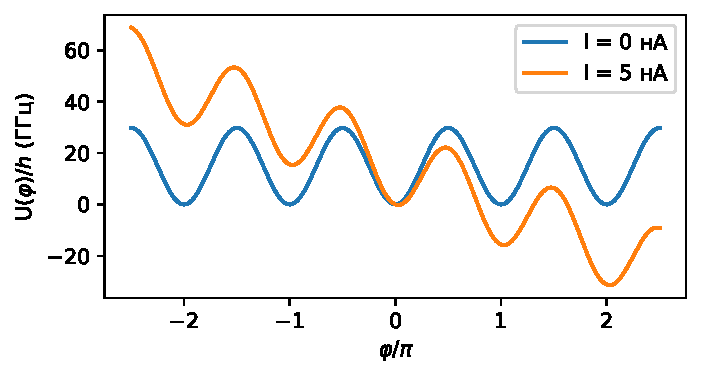
\includegraphics[width=0.7\linewidth]{Pictures/washboard}
	\caption{Потенциал ``наклонённого косинуса'', в котором происходит движение виртуальной частицы, описываемой уравнением \eqref{eq:rcsj_current}. Графики приведены для двух значений смещающего тока. Значение $E_J/h = 15$ GHz рассчитано для $I_c$ = 30 нА.}
	\label{fig:washboard}
\end{figure}

Такое уравнение можно решать классически, а в случае малых потерь и низкой температуры, пренебрегая диссипативным членом, составлять гамильтониан и квантовать его. Потенциальная энергия системы, описывающейся уравнением \eqref{eq:rcsj_current}, задается выражением (см. также \autoref{fig:washboard}):
\begin{equation}
	U(\varphi) = E_J\left(1-\cos \varphi - \frac{I}{I_c}\varphi\right).
\end{equation}
Константа $E_J$ получается из выражения для энергии идеального джозефсоновского перехода, рассчитываемого через уравнения Джозефсона и стандартное выражение для работы тока:
\begin{equation}
	U_J(\varphi) = \int_0^t V(\varphi) I(\varphi) \diff t = \frac{\hbar I_c}{2e}  \int_0^\varphi \sin\varphi \diff\varphi = E_J(1-\cos \varphi).\label{eq:josephson_energy}
\end{equation}
Значение же $\omega_0$ может быть выражено через величины $E_J$ и $E_C = e^2/2C$:
\begin{equation}
	\omega_0 = \sqrt{8 E_J E_C}.
\end{equation}
Используя данную формулу можно также прояснить смысл нелинейной джозефсоновской индуктивности. Эта величина вычисляется как обратное значение второй производной энергии системы по потоку (обобщенному импульсу) $\Phi = \int_{-\infty}^{t} V(\tau) \diff \tau = \frac{\Phi_0}{2\pi} \varphi$:
\begin{equation}
	L_J = \left(\frac{\diff^2 U_J(\varphi)}{\diff \Phi^2}\right)^{-1} = \left(\frac{\diff^2 U_J(2\pi \frac{\Phi}{\Phi_0})}{\diff \Phi^2}\right)^{-1} = \frac{\Phi_0}{2\pi I_c \cos \varphi}.
\end{equation}
В пределе малых $\varphi$ индуктивность оказывается равна $\Phi_0/2\pi I_c$, и формула для $\omega_0$:
\begin{equation}
	\omega_0 = 1/\sqrt{L_J C},
\end{equation}
что совпадает с привычным выражением для частоты колебательного контура.



\subsection{Макроскопическое квантовое туннелирование}

В 1985 году Мишель Деворе, Джон Мартинис и Джон Кларк провели эксперимент \cite{devoret1985measurements}, который окончательно позволил дать ответ на вопрос, допустимо ли квантовать уравнение на макроскопическую переменную $\varphi$ в уравнении \eqref{eq:rcsj_current} (первые подобные эксперименты проводились еще в 1981 году в IBM \cite{voss1981macroscopic}). Макроскопической она является потому, что однозначно определяет экспериментально детектируемый макроскопический ток, текущий через джозефсоновский переход. Таким образом, если квантовый аналог уравнения движения для джозефсоновского перехода действительно применим, то поведение его должно совпадать с поведением квантовой частицы в потенциале \autoref{fig:washboard}. Обнаружение такого поведения в указанной работе проводилось посредством охлаждения перехода до такой низкой температуры, что термические флуктуации оказывались меньше ожидаемых квантовых флуктуаций. 
Оба типа флуктуаций приводят к тому, что частица при определенном наклоне потенциала \autoref{fig:washboard} спонтанно покидает один из его уступов, в котором находилась изначально, и начинает скатываться вниз. Это означает, что контакт переходит в резистивное состояние с ненулевым переменным напряжением, определяемым значением производной разности фаз по закону \eqref{eq:JJ2}, которое можно обнаружить в эксперименте. По вероятности, с которой частица ``убегает'' из своего уступа в единицу времени, можно определить эффективную температуру $T_\text{esc}$ эквивалентных термальных флуктуаций, вызывающих такое ``убегание''. Понятно, что при нулевой температуре классическая частица остается в покое, пока сохраняется сколь угодно маленький уступ. Однако при наличии квантовых флуктуаций $T_\text{esc}$ окажется ненулевой даже для очень низких температур образца. 

Обнаружение макроскопического квантового туннелирования в джозефсоновских системах вызвало большой интерес и споры в научном сообществе. Например, в комментарии, вышедшем через 4 года\cite{silvestrini1989comment}, результат даже оспаривался на основании необъясненного постоянного сдвига $T_\text{esc}$ для двух переходов. Действительно, квантование переменной $\varphi$, которая уже сама по себе является квантовым числом \cite{ambegaokar1963tunneling}, не могло не вызывать удивления. Однако опираясь на дополнительные результаты, которые были получены за это время, авторы ответили на критику \cite{devoret1989devoret}, отметив большую систематическую погрешность для кривой, соответствующей классическому поведению и еще раз точность данных кривой квантового перехода. Также в своем ответе авторы отмечают еще одну работу 1988 года \cite{cleland1988measurement}, содержащую результаты исследования влияния диссипации на квантовое туннелирование: выяснено было, что низкодобротные джозефсоновские переходы, специально шунтированные тонкопленочными резисторами, демонстрируют подавление макроскопического туннелирования. Также во введении к работе отмечается, что реальные динамические потери в джозефсоновском переходе, определяемые эффективным сопротивлением $R$, в сверхпроводящем режиме не  равны $R_N$ -- т.н. нормальному сопротивлению, измеряемому по наклону вольт-амперной характеристики перехода выше критического тока. В дальнейших экспериментах уже со сверхпроводящими кубитами выяснится, что собственные потери маленьких джозефсоновских переходов оказываются в действительности очень малы \cite{paik2011observation}.

Описанные эксперименты также подтолкнули обсуждение корректного квантовомеханического формализма для описания диссипативных систем \cite{caldeira1985influence, walls1985effect}. Данный вопрос представляет большой интерес не только с точки зрения практического описания джозефсоновских систем, но оказывается напрямую связан с неразрешенной до сих пор проблемой перехода от квантовомеханического микроскопического мира элементарных частиц к классическому миру макроскопических объектов, из них состоящих \cite{walls1985analysis, zurek2009quantum}.



\section{Сверхпроводниковые кубиты -- искусственные атомы}

\subsection{Очерк развития области}

После обнаружения квантовомеханического поведения такой крупной по размеру физической системы, как джозефсоновский переход, научное сообщество оказалось заинтересовано возможностью использования её в качестве элемента квантовой вычислительной системы, концепция которой родилась также в 80-х годах \cite{manin1980, feynman1982simulating}. 

На самом деле уже в первых экспериментах по квантовому макроскопическому туннелированию был открыт первый сверхпроводниковый кубит -- фазовый, -- страдавший, правда, в то время от чрезвычайно быстрой релаксации при добротности измерявшихся систем не выше сотни. Несмотря на это обычно первым сверхпроводниковым кубитом называется т.н. зарядовый кубит на основе ящика куперовских пар \cite{nakamura1999coherent}, так как именно на нём в 1999 году были впервые продемонстрированы когерентные квантовые осцилляции заселенности двух состояний. Скорость релаксации в этой системе также была очень высока, поэтому для генерации импульсов товарищам Ясунобу Накамуре, Юрию Пашкину и Джао-Шеню Цаю пришлось использовать высокоскоростной цифровой генератор импульсов Anritsu MP1758A с временным разрешением порядка 5 пикосекунд -- серьезнейшую для того времени машину. 

Следом за зарядовым кубитом в 2000 году группой голландских и американских ученых был предложен и реализован потоковый кубит -- алюминиевое кольцо с тремя джозефсоновскими переходами, внешний поток через которое выставляется в $ \Phi_0/2 $ \cite{van2000quantum}. При таком внешнем потоке и ненулевой геометрической индуктивности кольца потенциал виртуальной частицы, о которой говорилось в предыдущем разделе, оказывается симметричным двухъямным с минимумами, отвечающими классическим состояниям с сверхтоками, текущими в противоположные стороны. За счет туннелирования через барьер между ямами энергетическое вырождение между классическими состояниями снимается, а основное и возбужденное состояния оказываются  ``кошками Шредингера'' -- коллективными суперпозициями большого числа частиц, доступными для измерения простыми приборами. Конечно, речь о том, чтобы приготовлять настоящих кошек в состояниях суперпозиции, не идет, так как они они являются гораздо более сложными системами и не обладают свойствами Бозе-конденсатов куперовских пар, обеспечивающими чрезвычайно слабую связь их с внешней средой. Однако и этот эксперимент, и многие другие последующие показали, что природа принципиально не запрещает суперпозиции состояний даже для очень большого числа частиц.

\begin{figure}
	\centering
	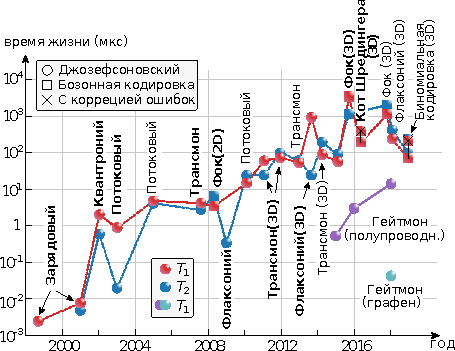
\includegraphics[width=.8\linewidth]{shoelkopfs_law.pdf}
	\caption{Иллюстрация ``закона Шелькопфа'', предсказывающего экспоненциальный рост времен релаксации и когерентности свехрпроводниковых кубитов с годами исследований. Адаптировано из обзора \cite{kjaergaard2020superconducting}. Полужирным шрифтом обозначены первые реализации указанных архитектур кубитов.}
	\label{fig:shoelkopfslaw}
\end{figure}

В 2002 году в группе ``Quantronics'' (от \textit{quantum electroninics}) Дэнисом Вионом и соавторами был реализован первый кубит, время фазовой когерентности которого приблизилось к 500 нс -- квантрониум \cite{vion2002manipulating}. Особенностью его было то, что он обладал двумя параметрами контроля частоты: напряжение на затворе, как у зарядовых кубитов на основе одноэлектронных транзисторов, и поток через контур, содержащий джозефсоновские переходы, как в потоковых кубитах. Также был реализован новый способ считывания через шунтирующий большой джозефсоновский переход, переходящий или не переходящий в резистивное состояние в зависимости от энергетического состояния кубита (в нём ни фаза, ни число куперовских пар не являются хорошо определенными переменными, и вычислительный базис строится на двух нижних собственных состояниях гамильтониана). Так как в то время еще не было полной теории, описывающей микроскопическую природу диссипации в подобных системах, в статье не указывается, какие именно решения позволили достичь увеличения времени когерентности. 

Также в 2002 году Джон Мартинис с соавторами работая в то время в Национальном Институте Стандартов и Технологии продемонстрировал когерентные осцилляции Раби на фазовом кубите \cite{martinis2002rabi} (джозефсоновский переход Nb/AlO$_x$/Nb). Когерентность кубита опять оказалась весьма низкой, порядка десятков наносекунд. Однако именно в этой работе было сделано предположение о том, что источником потерь является эквивалентный конденсатор джозефсоновкого перехода, в аморфном оксиде которого могут существовать дефекты, связывающиеся с кубитом. Интересно отметить, что примерно в то же время в Университете Канзаса проводились эксперименты на тех же кубитах, но с другим типом переходов -- NbN/AlN/NbN, и исследователи сообщали о совершенно невероятных для того времени временах когерентности в 10 мкс \cite{han2001time}, но по каким-то причинам исследования в той группе практически не продолжались.

Исследования причин потерь в джозефсоновских контактах продолжались, и в 2004 году были впервые открыты ``микроволновые резонаторы'', которые существенно уменьшали время когерентности кубитов на определенных частотах \cite{simmonds2004decoherence}. Уже тогда авторам было понятно, что скорее всего данные резонансы связаны с двухуровневыми квантовыми системами внутри перехода, хотя в строгом классическом смысле слова резонаторами такие системы назвать, конечно, было нельзя. Это открытие послужило отправной точкой для дальнейшей многолетней и кропотливой работы по подбору материалов и производственных циклов для создания сверхпроводникового квантового процессора.

Следующим шагом в экспериментах стала демонстрация так называемой квантовой электродинамики электрических цепей (\textit{circuit QED}) \cite{blais2004cavity, wallraff2004strong}. Название это было создано по образу квантовой электродинамики полостей (\textit{cavity QED}) -- области науки, впервые показавшей возможность управления изолированными одиночными квантовыми системами \cite{mabuchi2002cavity}. Архитектура, связывающая кубит с микроволновым резонатором позволяет осуществлять неразрушающее (проецирующее) измерение его состояния. Ранее такое измерение было возможно лишь для зарядовых кубитов \cite{lehnert2003measurement}, в то время как для потоковых и фазовых кубитов измерение СКВИДом было разрушающим -- приводило к нагреванию кубита и необходимости повторно инициализировать его в основное состояние. С потоковым кубитом резонатор удалось сильно связать в 2008 году \cite{abdumalikov2008vacuum}.

Квантовая электродинамика цепей открыла дорогу для новых типов кубитов. Поистине прорывным оказалось открытие в 2007 году того, что увеличение электрической емкости у сверхпроводящих островов зарядового кубита, означающее подавление зарядовой энергии в его гамильтониане, приводит к экспоненциальному подавлению зарядовой дисперсии (зависимости частот переходов между уровнями от наведенного на остров заряда) \cite{koch2007charge}. Новый тип кубита был назван трансмоном. Преодоление зарядового шума (в западной литературе встречается выражение ``life after charge noise'' \cite{houck2009life}) в свою очередь открыло новую огромную область исследований. В базе Web Of Science с момента первой публикации в 2008 году на текущий момент зарегистрировано более 450 публикаций с ключевым словом ``transmon''. Для потоковых кубитов идея шунтировать переход большой емкостью оказалась также плодотворной, позволив уменьшить зависимость от магнитного потока и, соответственно, дефазировку кубитов вызываемую потоковым шумом вне точки вырождения \cite{you2007low, yan2016flux}. Ключевая роль использования резонаторов для считывания заключается в том, что энергетические состояния трансмона, используемые в качестве вычислительного базиса, как и в фазовом кубите, оказываются неразличимы по заряду -- средний заряд на острове, шунтированном большой емкостью, оказывается нулевым как для основного, так и для возбужденного состояний. Однако эти состояния оказывается возможно различить по сдвигу частоты резонатора так же, как и в случае использования зарядовых или потоковых кубитов -- дисперсионное считывание оказалось универсальным средством.

В 2009 году был предложен очередной кубит -- т.н. флаксоний, представляющий собой контур с кинетической индуктивностью и джозефсоновским переходом \cite{manucharyan2009fluxonium}. По своей сути это ВЧ-СКВИД (сверхпроводящее кольцо с одним переходом), с тем лишь отличием, что индуктивность практически полностью набирается за счет кинетической части, реализованной при помощи цепочки джозефсоновских переходов. На таких кубитах продемонстрировано рекордное время релаксации в 8 мс при определенном значении внешнего магнитного потока за счет подавления туннелирования квазичастиц \cite{catelani2011relaxation, pop2014coherent}. Этот тип кубитов также поддается дисперсионному считыванию.

\subsection{Квантование цепей с джозефсоновскими переходами}

Квантование электрической цепи, содержащей джозефсоновские переходы, практически не отличается от квантования линейных цепей, описанных в работе \cite{devoret1995quantum}. Единственный дополнительный шаг заключается в расчете энергетического члена перехода \eqref{eq:josephson_energy}, в котором требуется правильным образом связать сверхпроводящую разность фаз $\varphi$ с потоковой переменной \eqref{eq:phi_variable}. Это можно сделать используя второй закон Джозефсона:
\begin{equation}
\begin{aligned}
	U_J(\varphi) = E_J (1-\cos\varphi) &= E_J\left(1 - \cos \left( \int_{-\infty}^{t} \frac{2e}{\hbar} U(\tau) \diff\tau\right)\right)\\
	&= E_J \left( 1 - \cos \left(\phi/\Phi_0\right)\right),
\end{aligned}
\end{equation}
где $\phi$ -- узловой поток на стороне перехода, которую мы не считаем землёй. Тогда в потоковом базисе энергия конденсатора, соединённого параллельно с переходом в RCSJ-модели, запишется как $C\dot\phi^2/2$. Далее из лагранжиана получаем гамильтониан одиночного перехода для обобщенного импульса (узлового заряда) $q = \partial \mathcal L / \partial \dot \phi = C \dot \phi$:
\begin{equation}
	\mathcal H = \frac{q^2}{2C} + E_J (1 - \cos (\phi/\Phi_0)),
\end{equation}
Далее, делая каноническое преобразование $\phi / \Phi_0\rightarrow  \varphi$, $q \rightarrow 2en$ и опуская постоянный член, получаем
\begin{equation}
{\mathcal{H}} = 4 E_C n^2  - E_J \cos \varphi,
\end{equation}
где $E_C = e^2/2C$ -- т.н. зарядовая энергия, а $n$ -- число протуннелировавших куперовских пар; таким образом и завершается переход от узлового потока к джозефсоновской разности фаз. Теперь, совершая процедуру канонического квантования на канонически сопряженных переменных $(n, \varphi)$, получим в операторном виде
\begin{equation}
\hat{\mathcal H}  =  4 E_C \hat n^2  - E_J \cos \hat \varphi,\label{eq:transmon_hamiltonian}
\end{equation}
что являет стандартное выражение для гамильтониана зарядового кубита (или трансмона, в случае $E_J \gg E_C$) \cite{koch2007charge}. Помня, что валентность преобразования к $\{\varphi, n\}$ равна $1/\hbar$, получаем  $ [\hat \varphi, \hat n] = i $, что отличается от более привычного коммутатора $ [\hat\phi, \hat q] = i\hbar $ на узловые потоки и заряды, но полностью согласуется с \eqref{eq:JJ1}, \eqref{eq:JJ2}. Отметим также, что точно такой же гамильтониан можно записать для математического маятника \cite{koch2007charge}.

Главным отличием этого выражения от результатов, полученных в разделе \ref{sec:circuit_quantization}, является необходимость квантования электрического заряда на узле с шагом $2e$. Действительно, через джозефсоновский переход может протечь лишь целое число куперовских пар, а через конденсатор ток не течет вообще. Однако в процедуре квантования мы до сих пор в явном виде не накладывали ограничения целочисленности на собственные значения $\hat n$. Для демонстрации того, что эта целочисленность автоматически встроена в уравнение Шредингера с гамильтонианом \eqref{eq:transmon_hamiltonian}, запишем его в фазовом представлении:
\begin{equation}
	\left(- 4 E_C \frac{\partial^2}{\partial \varphi^2} - E_J \cos \varphi\right)\psi_j(\varphi) = E_j \psi_j(\varphi).\label{eq:transmon_shroedinger_varphi}
\end{equation}
Если бы в этой задаче не было условия на область определения волновой функции, то решение уравнения Шредингера описывалось бы Блоховскими функциями в силу периодичности потенциала. Однако на самом деле решение уравнения должно быть строго $2\pi$-периодично по смыслу квазиимпульса $\varphi$. Поэтому естественным образом возможно разложить его в ряд вида
\begin{equation}
	\psi_j (\varphi) = \sum_n u_{jn} e^{i n \varphi}.
\end{equation}
Вспоминая, что волновые функции в представлениях канонически сопряженных переменных являются Фурье-образами друг друга, сразу получаем, что в зарядовом представлении собственные состояния достаточно разложить по счетному, а не континуальному базису состояний с дискретным значением протуннелировавшим зарядом $2en$. То же можно сказать и про разложение вообще любой периодичной волновой функции, не ограничиваясь собственными состояниями. И с другой стороны, квантование заряда в свою очередь обеспечивает $2\pi$-периодичность волновой фукнции в фазовом представлении, то есть на самом деле нельзя выбрать что-то одно в качестве основополагающего рассуждения -- оба подхода эквивалентны и самосогласованны \cite{thuneberg2013, devoret1995quantum}. В зарядовом представлении гамильтониан \eqref{eq:transmon_hamiltonian} может быть записан в проекторном виде как \cite{devoret1995quantum}
\begin{equation}
	\hat{\mathcal{H}} = 4 E_C \sum_{n=-\infty}^{+\infty} n^2 \ket{n}\bra{n} + \frac{1}{2}E_J \sum_{n=-\infty}^{+\infty} \left( \ket{n-1}\bra{n} + \ket{n}\bra{n-1} \right),\label{eq:transmon_shroedinger_n}
\end{equation}
где $n$ -- квантовое число, отвечающее узловому заряду.

\subsection{Анализ собственных состояний трансмонов}




\begin{figure}
	\centering
	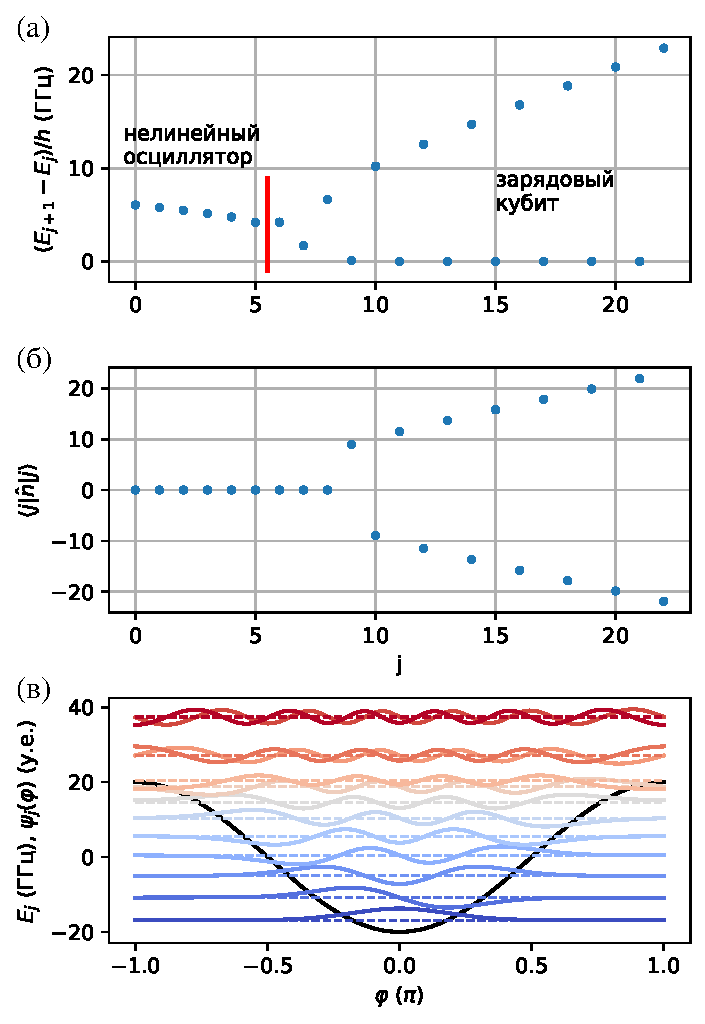
\includegraphics[width=0.6\linewidth]{Pictures/transmon_levels}
	\caption{(а) Разности энергий последовательных собственных состояний трансмона для $E_C/h = 250$ МГц, $E_J/h = 20$ ГГц. По линейному росту в правой части можно идентифицировать квадратичный закон дисперсии. (б) Переход от локализации к делокализации (от состояний осцилляторного типа к состояниям, близким к состояниями с определенным зарядом) происходит при данных параметрах при $j=9$. Расчет среднего значения числа пар после перехода производился для линейных комбинаций вырожденных состояний, дающих ненулевое среднее значение $\hat n = -i \partial/\partial \varphi$. (в) Волновые функции собственных состояний в фазовом представлении. Ноль каждой из $\psi_j(\varphi)$ смещен на величину соответствующей энергии $E_j$. Хорошо виден переход от осцилляторных состояний к состояниям-суперпозициям волн, бегущих в противоположные стороны (две верхние пары). Внутри каждой такой пары функции практически одинаковы с точностью до сдвига на $\pi/2$ относительно друг друга, и становятся всё ближе к синусоиде и косинусоиде с ростом $j$.}
	\label{fig:transmonlevels}
\end{figure}


Весьма подробный анализ собственных состояний, расчеты с помощью функций Матье и теории возмущений приведены в работе \cite{koch2007charge}. Мы же ограничимся лишь краткими рассуждениями общего характера и чуть более наглядными, чем в оригинальной работе, демонстрациями некоторых тезисов. На \autoref{fig:transmonlevels}~(а) изображен обработанный энергетический спектр уравнения \eqref{eq:transmon_shroedinger_varphi} с периодическими гранусловиями. На графике построены разности энергий пар последовательных уровней. Хорошо видны два режима системы: первый, низкоэнергетический, в классическом пределе представляет слабо нелинейные колебания вокруг нулевого тока, и второй режим, когда классический аналог -- маятник -- совершает вращение с ненулевой средней угловой скоростью. Второй режим для классической электрической системы означает наличие ненулевого среднего числа пар на острове. Численный алгоритм, работая в фазовом базисе, не находит комплекснозначные волновые функции такого типа, так как в любом случае собственные функции задачи Штурма-Лиувилля с действительными собственными значениями, коей является уравнение Шредингера \eqref{eq:transmon_shroedinger_varphi}, может быть сведено к действительному виду. Однако, как видно из \autoref{fig:transmonlevels}~(а), начиная с $j=9$ можно составить из последовательных пар действительных собственных функций, почти вырожденных по энергии, комплексные линейные комбинации вида почти плоских волн $e^{\pm i n \varphi}$, которые с хорошей точностью будут также являть собственными. Для таких комбинаций для $j\geq 9$ и проводится расчет среднего значения $\hat n$, показанного на \autoref{fig:transmonlevels}~(б). Таким образом, наглядно представляется, как именно происходит переход от локализованного к квазисвободному движению частицы в заданном периодическом потенциале. Первые 13 действительнозначных волновых функций для наглядности представлены на \autoref{fig:transmonlevels}~(в).

Для того, чтобы осуществлять контроль над состояниями трансмона, его связывают емкостно с микроволновой антенной. Для составления гамильтониана используется точно такая же процедура, как и в разделе \ref{sec:driven_lc}. Легко видеть, что возмущение пропорционально оператору числа пар $\hat n$, поэтому полезно будет изучить также его матричные элементы. На \autoref{fig:transmonnmelements} показан их модуль в зависимости от номеров собственных состояний, между которыми рассматриваются переходы. Видно, что вблизи малых $j$ оператор $\hat n$ по структуре практически пропорционален оператору $\hat a + \hat a^\dag$, отвечавшему заряду в планковском осцилляторе, однако начиная с $j\approx 5$ снимается запрет на переходы с пропусками состояний. Также, в отличие от осциллятора, в трансмоне могут происходить многофотонные переходы между состояниями даже в низкоэнергетическом подпространстве.

Чтобы выразить сходство между осциллятором и трансмоном, гамильтониан второго часто записывают в диагонализованном виде с использованием операторов рождения и уничтожения:
\begin{equation}
	\hat{\mathcal{H}}_{tr} \approx \omega_{ge} \hat a^\dag \hat a + \frac{1}{2}\alpha \hat a^\dag \hat a(\hat a^\dag \hat a - 1).\label{eq:transmon_nonlinear_ham}
\end{equation}
Здесь $\alpha$ -- ангармонизм \cite{koch2007charge}, определяющий наклон прямой, составленной из начальных точек на \autoref{fig:transmonlevels}~(a), а $\omega_{ge} \approx \sqrt{8 E_J E_C} - E_C$ -- это фундаментальная частота перехода между основным и первым возбужденным состояниями трансмона. Далее мы будем часто использовать обозначения $\ket{g},\ \ket{e},\ \ket{f},\ \ket{d}$ для первых четырех уровней трансмона, а также обозначениями $ge$, $ef$ для соответствующих однофотонных и $ef/n$ для соответствующих $n$-фотонных переходов. Понятно, что уравнение \eqref{eq:transmon_nonlinear_ham} работает лишь для низкоэнергетического подпространства. Также оно не учитывает зарядовую дисперсию, которая может оказаться существенной при достаточно малом $\alpha$ уже при $j \approx 4$ \cite{peterer2015coherence}.


\begin{figure}
	\centering
	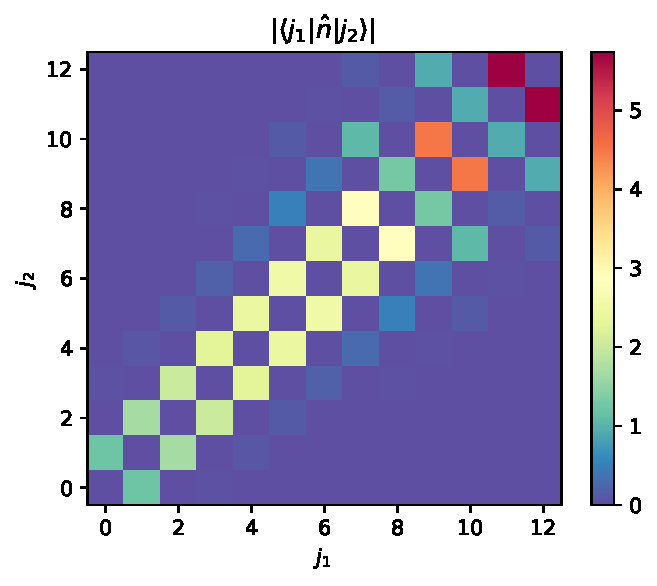
\includegraphics[width=0.5\linewidth]{Pictures/transmon_n_melements}
	\caption{Расчет модуля матричного элемента $\bra{j_1} \hat n \ket{j_2}$ для первых 13 энергетических состояний. Параметры расчета те же, что и для \autoref{fig:transmonlevels}.}
	\label{fig:transmonnmelements}
\end{figure}


\subsection{Расчет параметров цепей}

Для того, чтобы спроектировать образец, помимо квантовомеханических расчетов собственных состояний требуется провести классический электромагнитный расчет его параметров с учетом формы физических микроэлектродов. К примеру, рассмотрим трансмон типа Xmon \cite{barends2013coherent}, содержащий сверхпроводниковый остров в форме креста, отделенного от остальной металлизации нулевого потенциала зазором посредством плазмохимического травления через маску. Формы электрода острова и отделяющего его от земли зазора при идеальных условиях могут быть выбраны любыми, однако на практике для улучшения времен когерентности кубитов применяются геометрии, минимизирующие напряженность электрического поля в областях интерфейсов между металлической пленкой, из которой формируется остров, и кремниевой подложкой, а также между кремниевой подложкой и вакуумом (в зазоре) и, наконец, между металлом и вакуумом (над поверхностью пленки). Обычно, чем больше расстояния между электродами, тем шире пространственное распределение няпряженности полей; соответственно, основная энергия поля оказывается заключена в толще кремниевой подложки (концентрация силовых линий там происходит за счет большой $\epsilon \approx 12$ кремния), где концентрация дипольных дефектов в силу монокристаллической её структуры оказывается очень малой.

Для расчета емкости подобной крестообразной структуры можно приближенно применять формулы для погонной емкости копланарного волновода, однако это не точный и не универсальный метод. Для более точного электростатического расчета применяются специальные программы, например, FastCap или Ansys Maxwell. Также можно использовать программы и для электродинамического расчета наподобие Sonnet Suite -- тогда искомая емкость может быть извлечена из численно рассчитанного комплексного импеданса электрода относительно земли.

\section{Квантовая оптика со сверхпроводниковыми атомами}

Данный раздел посвящен основным экспериментам, которые удалось осуществить при помощи искусственных квантовых систем с момента первых опытов и до настоящего времени.

\subsection{Квантовая электродинамика цепей}

Упомянутая ранее основополагающая работа 2004 года из Йельского университета \cite{wallraff2004strong} по данным базы Web Of Science на текущий момент была процитирована в других работах всего около 2500 раз. Приведем из них наиболее существенные эксперименты, без учета обзоров, оказавшие наибольшее влияние на развитие области в целом. 

Первой работой, которую стоит отметить, является статья 2014 года от группы Джона Мартиниса, унивеситет Калифорнии, Санта-Барбара \cite{barends2014superconducting}. В этой работе была показана цепочка из 5 кубитов-трансмонов, над которыми были выполнялись однокубитные и двухкубитные операции типа сZ (\textit{controlled Z}, контролируемое вращение вокруг оси Z на сфере Блоха на угол $\pi$) с точностью, превышающей, соответственно, 99.9\% и 99.5\%. Работа имеет прямое отношение к статье 2004 года, так как важнейшая операция -- считывание состояний кубитов -- осуществлялось в эксперименте за счет дисперсионного взаимодействия резонатором. Это достижение позволило всерьез рассуждать о возможности масштабирования системы в той же архитектуре и всего через 5 лет привело в конечном итоге к экспериментальной демонстрации квантового превосходства в компании Google, нанявшей к тому времени весь коллектив Д. Мартиниса \cite{arute2019quantum}. Название работы 14 года содержит в себе предположение о том, что столь низкие уровни ошибок при управлении состояниями кубитов позволят вскоре осуществить их полное устранение путем применения алгоритмов коррекции \cite{shor1995scheme, fowler2012surface}, однако на текущий момент в научном сообществе нет четкого представления о том, как это будет реализовано на практике для большого числа кубитов \cite{kjaergaard2020superconducting}. Помимо Google исследования по квантовым вычислениям ведутся также и в IBM \cite{corcoles2015demonstration}.

Еще одной высокоцитируемой работой является эксперимент, выполненный группой немецких и испанских ученых, в котором потоковый кубит был сильно связан с несколькими модами микроволнового резонатора, причем энергия связи достигла порядка 10\% однофотонной энергии самих мод ($g/2\pi \sim 500$ MHz) \cite{niemczyk2010circuit}. Далее эксперименты по усилению связи и наблюдению отклонений от широко распространенной в квантовой оптике модели Джейнса-Каммингса были продолжены \cite{bosman2017multi}, и, в частности, привели к весьма интересным теоретическим результатам по устранению ультрафиолетовых расходимостей частоты \cite{gely2017convergence, malekakhlagh2017cutoff, parra2018quantum}.

Квантовая электродинамика цепей также позволила достичь большого прогресса в области управления состояниями квантовых осцилляторов. Основной вклад в это направление внесли ученые группы Мартиниса из университета Санта-Барбары и групп Шелькопфа и Деворе Йельского университета, от создания в резонаторах произвольных суперпозиций фоковских состояний \cite{hofheinz2009synthesizing} и ``кошачьих'' состояний \cite{vlastakis2013deterministically} из 100 фотонов (т.е, суперпозиций когерентных состояний излучения большой амплитуды) вплоть до коррекции ошибок в логическом кубите, построенном из сеточного состояния бозонной моды \cite{campagne2020quantum}.

Далее, в отдельное направление выделились работы касательно квантовой акустики, где кубиты связывались с акустическими пьезоэлектрическими резонаторами, работающими в квантовом режиме \cite{chu2017quantum, bolgar2018quantum}. На текущий момент также показана возможность управлять их квантовыми состояниями \cite{satzinger2018quantum}.

Наконец, интереснейшей областью является экспериментальное наблюдение квантовых траекторий. Впервые в 2011 году в лаборатории Квантовой наноэлектроники университета Бёркли под руководством проф. Ирфана Сиддики впервые пронаблюдали квантовые скачки кубита-трансмона, связанного с микроволновым резонатором \cite{vijay2011observation} (впервые такие эксперименты были проведены на отдельных ионах в ловушках еще в 1986 году). Прорывным этот эксперимент стал благодаря использованию параметрического усилителя в фазочувствительном режиме. Перед усилением считывание осуществлялось при помощи резонатора, фаза отражения сигнала от которого менялась на 180$ ^\circ $ в зависимости от состояния кубита. Установка была настроена таким образом, что при считывании состояния $ \ket{0} $ сигнал считывания попадал на параметрический усилитель в противофазе с сигналом накачки, ослабляя её. Когда же кубит оказывался возбужден, сигнал считывания, наоборот, усиливал накачку и при правильном подборе её мощности приводил к бифуркации усилителя и изменении фазы отражения мощного сигнала накачки также на 180$ ^\circ $. Таким образом авторы могли выполнять считывание состояний кубита при помощи одного импульса без усреднений и детектировать квантовые прыжки системы с соотношением сигнал-шум порядка 4 при непрерывном возбуждении её светом. В последующие годы исследования в области сильных квантовых измерений на сверхпроводниковых кубитах активно развивалась; наиболее весомыми работами оказались статьи о стабилизации осцилляций Раби посредством непрерывного слабого измерения \cite{vijay2012stabilizing}, восстановление отдельных квантовых траекторий по результатам слабых измерений  \cite{murch2013observing}, детектирование прыжков и возвращение системы в исходное состояние в реальном времени \cite{minev2019catch}.

\subsection{Квантовая микроволновая оптика ``на чипе''}

В то время как квантовая электродинамика цепей в основном работает с излучением, пойманным в резонатор (\textit{confined radiation}), существует целый набор физических эффектов, которые проявляются только при соединении атома с континуумом мод. В данной теме основополагающей является работа Олега Астафьева 2010 года касательно резонансной флюоресценции искусственного атома на основе потокового кубита, встроенного в одномерный микроволновый волновод \cite{astafiev2010resonance}: по данным WOS на 2021 год она процитирована более 400 раз. Среди работ, последовавших за ней, можно также выделить несколько наиболее цитируемых. Практически следом вышла статья о наблюдении эффекта электромагнитно-индуцированной прозрачности на потоковом кубите \cite{abdumalikov2010electromagnetically}, затем работы по исследованию микроволновой фотонной блокады \cite{lang2011observation}, однофотонным источникам на основе сверхпроводниковых атомов \cite{bozyigit2011antibunching,peng2016tuneable}, по исследованию состояний распространяющихся фотонов \cite{eichler2011experimental}, и т.д. Актуальный и весьма обширный обзор по теме, содержащий более 1000 ссылок, вышел в 2017 году \cite{gu2017microwave} и содержит 6 разделов, описывающих различные направления экспериментов в области, поэтому в этой главе мы не будем далее углублять перечисление результатов и перенесем обсуждение наиболее релевантных работ в следующие главы, относящиеся к непосредственно выполнявшимся автором экспериментам.

\section{Выводы по Главе 1}

Автором была показана историческая перспектива развития микроволновой квантовой оптики со сверхпроводниковыми искусственными атомами от истоков квантовой механики до актуальных исследований последних лет. 

\chapter{Автоматизация эксперимента}

\section{Обсуждение используемых инструментов}

Начиная с возникновения области сверхпроводниковых кубитов в конце  90-х годов, в силу веяний цифровой эпохи, эксперименты с ними так или иначе подразумевали использование компьютерной техники, будь то управление экспериментом или обработка данных. В последние годы в связи с серьезным усложнением структуры исследуемых квантовых систем (увеличение числа кубитов, числа линий, открытие возможностей для выполнения более сложных квантовых алгоритмов с ростом времен когерентности кубитов, необходимость автоматизации повторяющихся операций при масштабировании) серьезное компьютерное оснащение экспериментальных установок в нашей области стало необходимостью. Автор данной работы лично занимался разработкой и отладкой программного кода для управлением экспериментами начиная с 2014 года сначала в Лаборатории сверхпроводящих метаматериалов в НИТУ МИСиС, затем с 2015 года в Лаборатории искусственных квантовых систем в МФТИ, а также в лаборатории группы Устинова в РКЦ, расположенной в ИФТТ РАН в Черноголовке. 

Достаточно часто ученые используют программные пакеты типа Labview, которые не требуют навыков программирования и позволяют исполнять логику эксперимента с использованием графического интерфейса. Увы, такой подход не может быть применен для работы со сложными многокубитными схемами, так как не позволяет реализовать модульную гибкую архитектуру программ, пригодную к быстрой переработке и модернизации. Другие подходы, такие, как, например, среда Matlab, позволяют создавать текстовые программы, однако, не являясь полноценными языками общего назначения, проигрывают в гибкости и поддержке. Самым разумным выбором для проведения научных исследований сейчас признан язык Python, допускающий работу в парадигме объектно-ориентированного программирования и содержащий большое количество библиотек, специально предназначенных для научных расчетов. Серьезным недостатком этого языка является невысокая производительность, вызванная, в первую очередь, тем, что он является интерпретируемым, а не компилируемым. Это приводит как к дополнительным временным издержкам при любых операциях, так и к невозможности выполнять потоки с разделяемой памятью параллельно на нескольких физических ядрах. Однако, пока задержка эксперимента определяется приборами, непосредственно выполняющими измерения, это не является большой проблемой: за 7 лет работы автор не столкнулся с проблемами производительности, которые потребовали бы серьезной переработки кода или использования вставок на других языках. В частности это обеспечивается тем, что обычно вычисления производятся на самих приборах, либо тем, что данные экспериментов в основном имеют достаточно простую структуру и могут быть легко обработаны при помощи стандартных компилированных библиотек, к которым уже реализован высокопроизводительный интерфейс из Python. Однако, несмотря на этот опыт, нет гарантий, что в дальнейшем увеличивающиеся требования и использование более низкоуровневых приборов не потребуют перехода на более высокопроизводительные языки.

\section{Краткое описание экспериментальной установки и измерительных методов}

\subsection{Оснащение криостата растворения}

Центральной установкой, вокруг которой строится экспериментальная схема для работы со сверхпроводниковыми искусственными квантовыми системами, является рефрижератор растворения. В наших лабораториях используются коммерчески доступные (в условиях отсутствия санкций) приборы фирм Oxford (Великобритания) и BlueFors (Финляндия). Вторая фирма на момент написания ВКР является лидером в области и получает большое количество заказов со всего мира (в частности, в 2019 году более 100 рефрижераторов были заказаны Китаем исключительно для квантовых проектов). К сожалению, несмотря на то, что в их создании СССР был первопроходцем, после поражения в холодной войне такие приборы в России не производятся и государству приходится тратить огромные средства на приобретение их за границей (по нынешнему курсу BlueFors запрашивают до 50 млн. руб. за одну машину в комплектации с несколькими десятками сверхпроводящих коаксиальных линий). 

Криостат растворения сухого типа представляет собой вакуумную камеру, к которой подключен рефрижератор Гиффорда-Макмагона для получения первичной температуры в 4 К, необходимой для конденсации гелиевой смеси изотопов He3-He4. С 4 К до 10 мК охлаждение происходит сначала за счет откачки паров гелия, а затем благодаря осмотическому испарению из раствора одного изотопа в другой после их спонтанного разделения на две фазы \cite{wheatley1968principles, batey2015principles}. Внутри вакуумной камеры расположена последовательность уменьшающихся книзу металлических пластин, соединенных друг с другом полыми стальными стержнями. Теплопроводность нержавеющей стали при низких температурах очень мала, поэтому для равномерного охлаждения всех ступеней при первоначальном охлаждении до 4 К внутрь стержней путем подогревания адсорбента выпускается обменный газ; при достижении достаточно низкой температуры подогрев отключается, и обменный газ возвращается в адсорбент, разрывая тепловой контакт между ступенями, подлежащими охлаждению гелиевой смесью, и остальным устройством.

Внутри криостата проводятся коаксиальные линии для передачи микроволновых сигналов, а также шлейфы витых пар, которые могут использоваться для передачи низкочастотных сигналов и постоянного тока, например, при использовании магнитных катушек \cite{fedorov2017}. Материалы для изготовления проводов также требуются специальные, так как обычная медь является слишком хорошим проводником тепла, и использование её обычно приводит к невозможности достичь базовой температуры на нижней ступени. Превосходный обзор материалов, которые могут быть использованы при криогенных температурах в нашей области, дан в работе \cite{krinner2019engineering}. Автору известен только один случай, когда можно удачно использовать медные коаксиальные провода для проводки линий со ступеней в 1 К до 20 мК: это случай, когда такое соединение прерывается на каждой ступени стальным аттенюатором, которого оказывается достаточно. Важно помнить, что во всех случаях на каждой ступени требуется организовать хорошее тепловое соединение между проходящими сквозь нее линиями, будь то обмотка шлейфа витых пар вокруг медного якоря или использование аттенюаторов ослаблением 0 дБ, служащими исключительно для этой цели. Для термализации шлейфов автором также удачно применялись специальные переходные платы с широкими дорожками под паяльной маской, которые монтировались на медные уголки так, что дорожки плотно прилегали к металлу; данная конструкция оказалась достаточно удачной, хотя и требует уменьшения размера. 

На ступени 4 К требуется также разместить низкошумящие усилители, которые необходимы при работе со слабыми сигналами, несущими всего несколько фотонов энергии. В наших лабораториях используются усилители фирмы Low Noise Factory с различными полосами и шумовыми температурами (обычно около 2-4 К, что примерно в 20-40 раз хуже, чем квантовый предел при фазонечувствительном усилении на наших частотах). Такие усилители, как и криостаты, также производятся только за границей и стоят порядка 500 т. руб. за штуку. Так как в силу слабости измеряемых сигналов выходящие линии нельзя оснащать аттенюаторами, для защиты образцов от шумов усилителя, требуется использовать криогенные изоляторы или циркуляторы, которые также часто являются импортными и в таком случае стоят около 300 т. руб за штуку (фирмы-производители Quinstar, Raditek). Сейчас появились криогенные изоляторы отечественного производства Феррит-Квазар, не уступающие западным аналогам, однако выигрывающими по стоимости в 5 раз. Также используются микроволновые фильтры фирмы Minicircuits, которые хоть и не являются криогенными, тем не менее работают при сверхнизких температурах штатно. Также используются кустарные инфракрасные фильтры нижних частот, которые препятствуют распространению терагерцовых и инфракрасных сигналов по коаксиальным проводам.

\subsection{Электроника при комнатных условиях}

Всё управление физическими процессами, происходящими на чипе, производится при помощи электрических импульсов. Это могут быть как СВЧ-импульсы с несущей на частоте порядка 5 ГГц, так и импульсы постоянного тока. Текущие архитектуры компоновки сверхпроводниковых кубитов позволяют осуществлять однокубитные и двухкубитные операции за времена порядка десятков наносекунд, что определяет требования к управляющей электронике: необходима частота дискретизации порядка 1 Гвыб/с и схожая аналоговая полоса. Для генерации импульсов на СВЧ практически повсеместно используется схема повышения частоты на квадратурных смесителях с подавлением несущей и одной боковой полосой. Для считывания состояний кубитов при помощи дисперсионного взаимодействия с резонатором используется супергетеродиная схема на основе аналогичных методов повышения и понижения частоты. Во многих экспериментах по спектроскопии используется векторный анализатор цепей, который реализует калиброванную супергетеродинную схему внутри себя и позволяет получить относительное изменение амплитуды и фазы сигналов при прохождении через измерительный тракт. Помимо этого для контроля частоты используются прецизионные источники тока, однако часто предъявляемые к ним специалистами из нашей области требования чрезвычайно низких шумов часто оказываются излишними: при достаточно малой взаимной индуктивности между кубитом и управляющей линией можно использовать в качестве источника тока даже обычный ЦАП генератора импульсов произвольной формы практически не замечая влияния на скорость дефазировки, вызванной магнитными шумами.

В наших лабораториях используются приборы фирм Keysight (бывший Agi-lent, Rohde\&Schwartz, Tektronix, Yokogawa, Zurich Instruments, National Instr-uments, SignalCore, Spectrum. Самыми дорогими приборами являются векторные анализаторы цепей (до 8 млн. руб за штуку) и цифровые генераторы непрерывных сигналов СВЧ диапазона (до 3 млн. руб в зависимости от комплектации). Также используются микроволновые анализаторы сигналов (спектроанализаторы, 2 млн. руб), высокочастотные осциллографы (2 млн. руб), генераторы импульсов произвольной формы (1 млн. руб). Также используются шасси PXI с контроллером (встроенным компьютером) и без (подключается к внешнему компьютеру); первый вариант является гораздо менее рациональным, так как стоимость контроллера при тех вычислительных возможностях и меньшей гибкости завышается не менее чем в 5 раз. Гораздо более адекватным является вариант с карточкой, вставляющейся в системный слот и позволяющей подключить шасси к обычному компьютеру по проводам PCIe (в ПК также должна быть установлена специальная карта). Также есть карточки, вставляющиеся в периферийные слоты, позволяющие соединить несколько шасси в архитектуре ``гирлянды'' (\textit{daisy-chain}). В шасси может быть смонтировано порядка десятка приборов в гораздо более компактном форм-факторе по сравнению с приборами в самостоятельном исполнении. например, векторные анализаторы и анализаторы сигналов в формате PXI оказываются примерно в 5-10 раз меньше по размеру. Также в формате PXI коммерчески доступно большое число дешевых карточек высокоскоростных ЦАП и АЦП. Вкупе с гораздо большей (в десятки и сотни раз) пропускной способностью интерфейса PCIe по сравнению с традиционно используемыми GPIB, USB или Ethernet, применение шасси PXI должно быть максимальным.

\subsection{Измерительные методы}

Измерения образцов искусственных квантовых систем обычно начинаются с микроволновой спектроскопии. На \autoref{fig:workflow} схематически изображена процедура измерения сверхпроводниковых кубитов со считыванием через резонаторы. На первой панели изображен результат спектроскопии резонатора, которая выполняется векторным анализатором цепей; $S_{21}$ -- комплексный коэффициент пропускания через образец (амплитудно-фазо-частотная характеристика, АФЧХ), $f_p$ -- частота, на которой подается сигнал спектроскопии. По результатам измерения определяются положение резонансного пика и область сканирования $\Delta f_p$ вокруг него, которая затем используется для выполнения однотоновой спектроскопии. Область сканирования зависит от ширины резонансного пика, то есть от полной добротности \cite{fedorov2017} резонатора, но определяется ею не полностью. Как видно из второй панели, при выполнении однотоновой спектроскопии (ОТС) в зависимости от некоторого параметра (в дальнейшем мы будем называть его током $I$, изменяющим магнитный поток через некоторое кольцо кубита, и тем самым, его энергию) изменение частоты резонатора вследствие взаимодействия с кубитом может быть во много раз большим, чем его ширина. Эту проблему можно частично решить, если измерение проводить не на прямоугольной области параметрического пространства $\{f_p, I\}$, а записывать только фиксированную область вокруг резонанса, которая будет смещаться вместе с ним. Здесь может возникнуть проблема в областях, где резонансный пик оказывается не виден, как в случае на рисунке, но её также можно решить, усложнив логику программного кода. При ручном проведении измерений после завершения однотоновой спектроскопии экспериментатор примерно вычисляет горизонтальные координаты минимумов и максимумов частоты кубита (т.н. благоприятных точек, \textit{sweet-spots}), определяет период по потоку и переходит к двухтоновой спектроскопии (ДТС). 


\begin{figure}
	\centering
	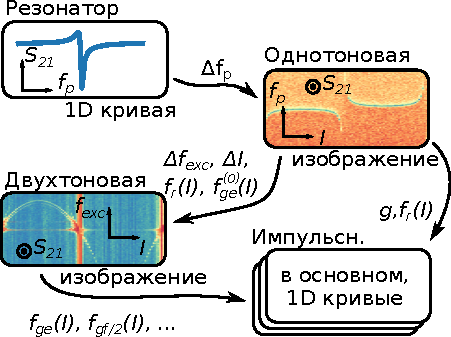
\includegraphics[width=0.5\linewidth]{Pictures/workflow}
	\caption{Схематическое изображение последовательности измерений при экспериментах с образцами квантовой электродинамики цепей со считыванием через резонатор.}
	\label{fig:workflow}
\end{figure}

Параметрами двухтоновой спектроскопии являются область сканирования частоты дополнительного, возбуждающего, микроволнового сигнала $\Delta f_{exc}$, область сканирования по току $\Delta I$, в которой ожидается наблюдение спектральной линии кубита, а также положение резонансного пика $f_r(I)$, в который при любом токе должен быть нацелен сигнал первого, считывающего, тона. Для выбора $\Delta f_{exc}$ таким образом, чтобы область сканирования с первого раза целиком захватила линию кубита, необходимо из данных ОТС заранее выяснить приблизительную зависимость его частоты от тока, $f_{ge}^{(0)}(I)$. Оказывается, что это возможно сделать с помощью компьютерного анализа данных ОТС, чему посвящена одна из работ автора \cite{fedorov2019automated} и к чему мы вернемся в следующих разделах. Результатом ДТС также является изображение, которое в зависимости от мощности возбуждающего сигнала может содержать достаточно сложную систему спектральных линий. При исследовании трансмонов необходимо извлечь из них те, которые соответствуют переходам $ge,\ gf/2,...$ \cite{fedorov2017}. При измерении в ручном режиме это делается на глаз, по положению наиболее яркой точки самой верхней кривой, обладающей правильной зависимостью от тока, и не представляет сложности для опытного экспериментатора. Однако при автоматизации этого шага возникают серьезные трудности, так как из-за шума и посторонних спектральных линий, а также необходимости аппроксимировать сразу несколько кривых одновременно, стандартные методы численного приближения кривых оказываются неустойчивы. Автором был разработан метод, совмещающий подходы преобразования Хафа \cite{hough1962} и алгоритма консенсуса случайной подвыборки (\textit{RANSAC}) \cite{fischler1981}, который позволяет с достаточной устойчивостью обнаруживать необходимые кривые при очень малом соотношении сигнал-шум, а также игнорировать паразитные спектральные линии. О деталях алгоритма мы также будем отдельно говорить в следующих разделах.

Наконец, после выполнения спектроскопии и определении основных физических параметров квантовой цепи, можно приступать к импульсным измерениям, результатами которых, по большей части, являются двумерные графики, не представляющие трудностей при обработке стандартными методами наподобие функции \textit{scipy.optimize.curve\_fit}. Дополнительным методом калибровки мощности считывания перед импульсными измерениями может быть эксперимент со Штарковским сдвигом переменного поля (AC-Stark effect) \cite{schuster2005ac}, который также дает изображение; однако оно обрабатывается сравнительно просто и потому этот эксперимент не будет детально рассматриваться в работе.

На текущий момент нами были кратко обозначены основные эксперименты, а именно одно- и двухтоновая спектроскопии, встречающие действительно серьезные проблемы при автоматизации, и именно про них речь будет идти в дальнейшем. Однако также стоит уделить внимание и общей архитектуре программного кода, который был разработан автором для автоматического измерения времен когерентности однокубитных образцов, о чем пойдет речь в следующем разделе.

\section{Архитектура измерительного программного кода}

Измерительное оборудование управляется набором программ из среды \foreignlanguage{english}{\textit{Jupy-ter}} языка \foreignlanguage{english}{Python}. Исходный код можно найти на сайте GitHub \cite{fedorov2021github}. Реализация всех процедур основана на объектно-ориентированной парадигме, в которой классы объектов разделены глобально на две группы: высокоуровневые драйверы приборов и отдельные измерения или группы измерений, оперирующих этими приборами. 

Драйверы приборов основаны на поставляемых библиотеках от производителей оборудования. Часто они опираются на язык SCPI и интерфейс NI-VISA, для которого используется сторонняя библиотека с открытым исходным кодом \textit{pyvisa} (в основном, это приборы в форм-факторе ``коробки''). Для приборов в формате PXI часто низкоуровневые драйверы реализованы как разделяемые библиотеки на C++; для них требуется использовать библиотеку \textit{ctypes}, чтобы вызывать функции C++ из Python. Это труднее, чем работа с SCPI, зато скорость обмена данными вырастает на порядки. В целом, классы драйверов в силу больших различий между приборами не создавались как наследники некоего общего абстрактного класса и практически не несут общих функций и не содержат патологических копий одного и того же кода. Однако, если бы Python поддерживал концепцию интерфейсов, как в типизованных языках, то можно было бы выделить несколько методов, которые присущи каждому из приборов. В нашей архитектуре главным из них является метод \textit{set\_parameters}, который получает на вход словарь, содержащий ключи -- имена параметров -- и их значения. Для многих приборов, например, оцифровщика Spectrum, внутри данного метода содержится еще и довольно сложная логика, которая автоматически увязывает конфигурацию прибора с тем набором параметров, который был передан, чтобы прибор не оказался в неправильном состоянии. Таким образом, видно, что работа с измерительным программным кодом драйверов осложняется здесь не только тем, что он является \textit{stateful} не только на уровне кода, но и на физическом уровне. Это осложняет юнит-тестирование, так как для составления тестов надо досконально знать, как будет реагировать прибор на ту или иную комбинацию параметров, и, следовательно, отладка может занимать достаточно долгое время.

Здесь стоит также отметить и драйверы приборов, которые были реализованы автором для дисперсионного считывания с помощью оцифровщика. Основным здесь является класс для виртуального векторного анализатора, собранного из четырех активных приборов (микроволнового генератора, ЦАП и АЦП, спектрального анализатора) и трех пассивных (два квадратурных смесителя, делитель мощности), описанный в файле \foreignlanguage{english}{\textit{DacAdcVNA.py}}; также был реализован векторный генератор на основе микроволнового источника, смесителя, ЦАП и того же спектрального анализатора (файл \foreignlanguage{english}{\textit{IQVectorGenerator.py}}). Основным свойством этих приборов является то, что они содержат предварительную калибровку квадратурных смесителей и выдают импульсный сигнал заданной по запросу амплитуды и фазы. Здесь стоит отметить, что ЦАП и АЦП в векторном анализаторе имели разную частоту сэмплирования, а именно, 1.25 Гвыб/с и 1 Гвыб/с, что, вопреки ожиданиям, не приводило к большому джиттеру порядка 1 нс. Погрешность фазы на 100 МГЦ ПЧ составляла при тестировании порядка 1 градуса при использовании синусоидального синхросигнала PXI частотой 10 МГц.

Группа классов для измерений опирается на двух общих родителей: \foreignlanguage{english}{\textit{Measurement}} и \foreignlanguage{english}{\textit{MeasurementResult}}. В первом классе реализуется выделение динамической визуализации и логики работы с приборами в два отдельных потока (благодаря внутреннему устройству библиотеки Matplotlib это позволяет добиться удвоения производительности несмотря на GIL). Также он указывает несколько методов, которые должны имплементироваться или переопределяться в дочерних классах (например, методы \foreignlanguage{english}{\textit{set\_fixed\_paremeters}} для указания параметров, обеспечивающих постоянный контекст эксперимента, и \foreignlanguage{english}{\textit{set\_swept\_parameters}}, в котором указывается, что именно и как будет изменяться перед считыванием данных). В конструктор объектам этого класса передается также набор объектов приборов в виде словаря или нескольких именованных аргументов; после этого они записываются в рефлексивно именуемые соответственно ключам или именам поля.

В \textit{MeasurementResult} указана структура данных для всех экспериментов (это словарь с ключевыми словами -- названиями перебираемых параметров -- и их значениями, а также многомерным массивом для результатов измерения). Важнейшей частью является описание интерфейса визуализации, который должен поддерживать статическую генерацию графиков по окончании измерения или просмотре старых данных и динамическую обновляемую визуализацию при идущем измерении. Последняя реализована при помощи функционала \textit{FuncAnimation} библиотеки \textit{matplotlib} и является достаточно производительной для того, чтобы без проблем обновлять тепловые карты размером более, чем 1000$\times$1000 точек.

Наследники этих двух классов описывают все то, что умеет делать измерительная установка, но с определенными оговорками. Часто оказывается так, что некоторые измерительные классы пишутся для определенной комбинации приборов, поэтому оказываются непригодны в другой лаборатории или при изменении архитектуры на физическом уровне. Также достаточно тяжело вести разработку кода, когда параллельно несколько групп ведут измерения совершенно разных образцов поочередно на одних и тех же приборах. В какой-то степени помогает контроль версий, однако все равно требуется найти более работоспособные подходы для организации всей системы на мета-уровне. Также трудно использовать один и тот же код в различных лабораториях, так как в некоторых приборах одной лаборатории есть несовместимости, требующие установки в код дополнительных условий или логики, которые не нужны для их аналогов во второй, что сильно ухудшает его понятность для людей, работающих исключительно там. Также тяжело переходить с одной архитектуры образца на другую, особенно, если изменяется оснастка, например, при добавлении параметрических усилителей. Несмотря на то, что изначально архитектура задумывалась универсальной, нет гарантий, что она потребует серьезной переработки в случае усложнения установки. Так, например, определённая работа потребовалась для переведения кода от однокубитных к многокубитным образцам -- теперь по каждому типу прибора при создании объекта измерения передается массив объектов, которые отвечают уже нескольким одинаковым физическим устройствам, управляющим соответствующими кубитами. Все эти проблемы вызваны тем, что есть неустранимая пропасть между кодом и физическим уровнем эксперимента, которая закрывается вручную экспериментатором, поэтому при подборе кадров требуется обязательно учитывать навыки программирования, которые будут применяться для ad-hoc решения упомянутых проблем. В дальнейшем пригодился бы опыт разработчиков интегральных микросхем, которые наверняка сталкиваются с похожими проблемами при переходе от одной микроархитектуры к другой.

Наконец, кратко опишем систему для автоматического измерения времен когерентности однокубитных образцов. В программном коде она состоит из нескольких классов, которые находятся в общем пакете под названием \textit{fulaut}. Параметры, которые требуется задать вручную храняться в файле \foreignlanguage{english}{\textit{experiment\_ parameters.json}}. Основным классом является \textit{MeasurementRunner}, который несет в себе общую структуру измерений. За предварительных поиск резонаторов, согласно \autoref{fig:workflow}, отвечает класс \textit{ResonatorOracle}. Он устроен достаточно просто и лишь ищет на развертке векторного анализатора необходимое число пиков, медленно уменьшая пороговую высоту пика на графике задержки (производной фазы по частоте). Такой подход работает одинаково для резонаторов как и шунтирующих, так и подключенных на отражение \cite{probst2015efficient}. Возвращает он области сканирования $\Delta f_p$ шириной порядка 5 ширин соответствующего пика. Далее, однотоновая спектроскопия выполняется классом \textit{STSRunner}. Здесь многократным измерением производится попытка подобрать правильные диапазоны по току и частоте $f_p$, т.к., как обсуждалось ранее, последний не всегда удается подобрать исключительно детектором резонаторов. Здесь впервые применяется класс для распознавания однотоновых спектров (\textit{AnticrossingOracle}), детали которого мы опишем ниже. Далее, по результатам распознавания запускается двухтоновая спектроскопия (класс \textit{TTSRunner}) в окрестности верхнего или нижнего свит-спота кубита-трасмона. Это измерение уже однократное, и после него сразу запускается детектор двухтоновых спектров (\textit{SpectrumOracle}), который также будет обсуждаться ниже. Если он успешно распознает спектр кубита, запускается измерение эффекта Штарка переменного сигнала для определения мощности считывания, и далее импульсные измерения. На этом этапе есть тонкость: в текущей реализации эффект Штарка промеряется лишь в одной оптимальной точке и именно там позволяет найти истинную несмещенную частоту кубита. Однако в других точках из-за изменения отстройки частот кубита и резонатора штарковский сдвиг также изменяется, что означает невозможность получения несмещенного спектра простым сдвигом аппроксимированной кривой на величину сдвига в оптимальной точке. Проводить калибровку эффекта Штарка в каждой точке по току чрезвычайно затратно по времени, поэтому было бы лучше применять аналитическое выражение для корректировки спектра по одному лишь значению в оптимуме частоты. Другой альтернативой может стать проведение двухтоновой спектроскопии в импульсном режиме, когда считывание и возбуждение разделены по времени, и первое не изменяет частоту кубита во время действия второго.

Импульсные измерения могут выполняться как при фиксированном значении частоты, так и в режиме прохода по частотам и использованием данных двухтоновой спектроскопии. Во втором случае могут возникнуть проблемы с попаданием в частоту в силу предыдущего рассуждения о токо-зависимом штарковском смещении двухтонового спектра. В любом случае, частота кубита, полученная их спектроскопии, оказывается недостаточно точной для проведения аккуратных измерений времен когерентности (например, видность осцилляций Раби при нерезонансном возбуждении оказывается понижена), поэтому перед выполнением чистовых измерений необходимо получить осцилляции Рамзи и вычислить их частоту путем аппроксимации моделью. Для этого требуется прежде всего получить осцилляции Раби в зависимости от длительности возбуждающего импульса и по их частоте определить длительность $\pi$-импульса. Этот эксперимент можно также делать в амплитудном режиме, наблюдая осцилляции Раби в зависимости от амплитуды импульса. После этого можно проводить эксперимент Разми с импульсами $\pi/2$; из частоты осцилляций напрямую вычисляется модуль отстройки несущей импульса от частоты кубита \cite{fedorov2017}. Так как для уточнения частоты модуля отстройки недостаточно, перед экспериментом Рамзи вводится искусственная отстройка порядка 10 МГц вниз, предполагая, что ошибка определения частоты по спектру будет меньше этого значения. В таком случае наблюдение осцилляций частотой менее 10 МГц будет означать превышение частоты несущей над частотой кубита, и наоборот. После определения частоты производится уже чистовое измерение осцилляций Раби, осцилляций Рамзи (оттуда извлекается время когерентности $T_2^*$), релаксации (время $T_1$), спинового эха Ханна ($T_{2E}$).

\section{Компьютерное распознавание результатов однотоновой спектроскопии}

\subsection{Введение}

Расчеты на квантовым компьютере подразумевают управление большим числом физических квантовых битов (кубитов). Одна из наиболее значительных проблем в этой связи заключается в том, что по сравнению с естественными кубитами на основе, например, ионами в ловушках, сверхпроводниковые кубиты создаются искусственно человеком. Это приводит к тому, что их параметры не воспроизводятся идеально, а, значит, и управление каждым из них в некоторых аспектах также должно индивидуализироваться. В большинстве случаев настройки системы управления определяются физическими параметрами образца, которые для каждого из них выясняются in situ при помощи последовательности калибровочных измерений \cite{kelly2018physical, chen2018metrology, fedorov2019automated}. Естественно, эти измерения должны быть автоматизированы, иначе при увеличении числа кубитов этот шаг окажется ``бутылочным горлышком'' по производительности, не говоря о неизбежности ошибок при ручном выполнении алгоритма. Более того, автоматическая система сама может проводить повторные калибровки в случае, если обнаружатся аномалии в результатах измерений, вызванные дрейфом физических характеристик образца. Автоматизация особенно полезна в условиях развития и становления архитектур чипов, а также методов изготовления, когда архитектура не меняется, но изменяются технологические шаги и производятся многочисленные измерения. Последний случай требует особой воспроизводимости измерений, которой можно добиться исключительно при полной их автоматизации.

Как уже говорилось ранее, ведущей архитектурой для создания квантовых процессоров на основе сверхпроводниковых кубитов сейчас является квантовая электродинамика цепей, в которой каждый кубит соединяется с резонатором, через который производится считывание его состояний. Автор предложил и реализовал несколько методов компьютерного зрения, делающих возможной автоматическую калибровку таких ячеек при осуществлении однотоновой и двухтоновой спектроскопии. Здесь под компьютерным зрением понимаются алгоритмы, использующие статистические методы для интерпретации данных на основе моделей, использующих геометрию, физику и теорию обучения \cite{forsyth2012computer}; из \autoref{fig:workflow} видно, что по крайней мере два типа экспериментов дают на выходе изображение, поэтому вполне естественно использовать методы компьютерного зрения для из обработки. Условиями для применимости таких методов являются их точность, высокая производительность и устойчивость к шумам, а также общность подхода, обеспечивающая возможность их применения для различных типов кубитов с минимальными модификациями программного кода.

\subsection{Теоретическая модель однотонового спектра}\label{sec:sts_theory}

Ниже мы переходим к рассмотрению алгоритма, служащего для распознавания данных однотоновой спектроскопии. Мы ограничиваемся широко используемым случаем \cite{kelly2015state, versluis2017}, когда резонатор связан с одним кубитом, в котором теоретическая зависимость частоты резонатора оказывается строго периодической по магнитному потоку. Если кубитов два или более, в случае значительных перекрестных взаимодействий зависимость частоты резонатора окажется апериодической, как при совмещении двух периодических сигналов с неизвестным отношением периодов; это серьезно осложнит определение параметров системы. Поэтому в этом случае разумно будет прежде всего добиться отсутствия паразитных взаимодействий, а потом применять предложенный автором метод при перестройке лишь одного кубита из набора присоединенных к резонатору.

\begin{figure}
	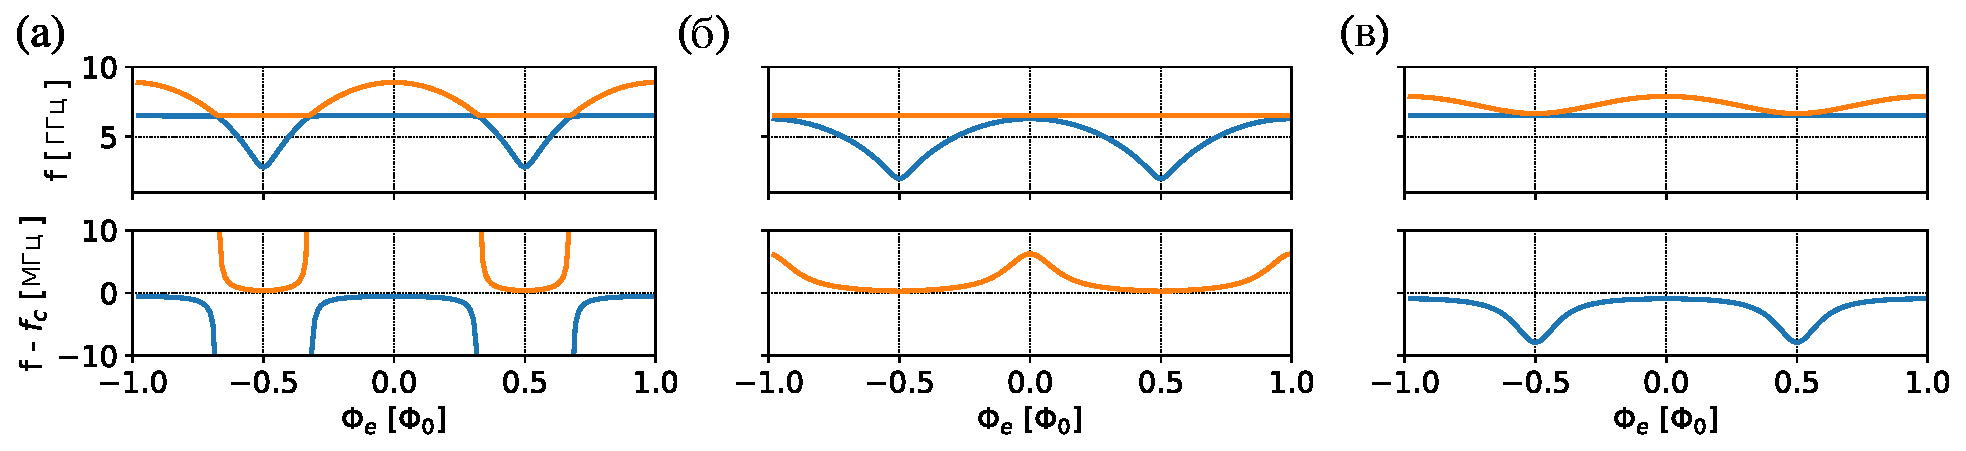
\includegraphics[width=1\linewidth]{Pictures/anti_theor}
	\caption{Три случая взаимного расположения перестраиваемой потоком частоты кубита (на примере трансмона) и частоты резонатора. Нижний ряд показывает увеличенную область вокруг собственной частоты резонатора $f_c$. (а) Частота кубита проходит через частоту резонатора, образуя квазипересечение. (б) Кубит находится под резонатором по частоте, изгибая его линию вверх при приближении к верхней оптимальной точке. (в) Кубит находится выше резонатора, изгибая его линию вниз при приближении к нижней оптимальной точке.}
	\label{fig:antitheor}
\end{figure}

Модельные кривые, показывающие частоты переходов из основного состояния на первые два возбужденных при диагонализации модели Джейнса-Каммингса для кубита со спектром трансмона \cite{blais2004cavity, koch2007charge, filipp2011multimode}, изображены на \autoref{fig:antitheor}. Как видно, есть всего три возможных случая взаимного расположения кубита и резонатора: один с квазипересечением и два без него. Мы увидим в дальнейшем, что наибольшую трудность представляет именно первый случай из-за разрывности модельной функции, которая хорошо видна на нижнем графике \autoref{fig:antitheor}~(а).

Джозефсоновская энергия трансмона с учетом возможной асимметрии его СКВИДа (см. \eqref{eq:Ic_squid_asym}) в зависимости от магнитного потока $\Phi_e$, проходящего через него, может быть описана следующей формулой:
\begin{equation}
\begin{aligned}
E_{J}(\Phi_e) &= E_{J\Sigma} \cdot k(d, \Phi_e),\\
k(d, \Phi_e) &= \left[\cos^2\left(\frac{\pi \Phi_e}{\Phi_0}\right) +d^2 \sin^2 \left(\frac{\pi \Phi_e}{\Phi_0}\right)\right]^{\frac{1}{2}},
\label{eq:EJ_Phie}
\end{aligned}	
\end{equation}
где $E_{J\Sigma} = E_{J1}+E_{J2}$ ($E_{J1},\ E_{J2}$ -- джозефсоновские энергии каждого из переходов), а $d = \frac{E_{J1}-E_{J2}}{E_{J1}+E_{J2}}$ -- значение асимметрии. Как видно, периодом зависимости является $\Phi_0$. В таком случае, используя приближенные аналитические выражения для уровней энергии трансмона \cite{koch2007charge} при малости отношения зарядовой и джозефсоновской энергий, можно получить выражение для частоты перехода $ge$ трансмона $f_{ge}$ в зависимости от $\Phi_e$:
\begin{equation}
	f_{ge}(\Phi_e) \approx  f_{ge}^\text{max} \cdot \sqrt{k(d, \Phi_e)},
\end{equation}
где $f_{ge}^\text{max}$ -- максимальная частота в верхней оптимальной точке, равная $$\sqrt{8E_J(0) E_C} - E_C.$$
Погрешность данной формулы зависит от магнитного потока и описывается выражением 
\begin{equation}
	\left[\sqrt{k(d, \Phi_e)}-1\right] \cdot E_C,
\end{equation}
которое принимает значительные значения, если одновременно $d \ll 1$ и $\Phi_e \approx \Phi_0/2$, то есть когда эффективная джозефсоновская энергия достаточно мала. Однако в этом случае оказывается неточным и приближение для самих уровней энергии, так что вообще говоря при данных условиях нет аналитической модели, правильно описывающей частоту трансмона. Однако для наших целей полученное выражение весьма удобно, так как при малом $E_J$ кубит обычно далеко отстроен от резонатора и незначительно влияет на него, а в остальных областях точность его достаточна. Более того, приближенное выражение зависит только от двух параметров $(f_{ge}^{\text{max}}, d)$, в то время как полное зависит от трех $(E_C,\ E_{J1},\ E_{J2})$. 

Также стоит отметить, что в реальном эксперименте магнитный поток $\Phi_e$ может быть известен с точностью до линейного отображения. Экспериментатор может контролировать только параметр прибора, например, ток на источнике, который будет связан с потоком как $\Phi_e = M I + \Phi_r$, где $ M $ обозначает взаимную индуктивность между линией контроля и петлёй СКВИДа, а $\Phi_r$ -- остаточный магнитный поток, определяющийся неидеальностью установки и образца. Поэтому когда речь будет касаться экспериментальных данных вместо потока мы будем использовать в качестве параметров модели ток $I$, период по току $\Pi = \Phi_0/M$ и ток оптимальной точки $I_{ss} = - \Phi_r/M$.

Установив математическое описание спектральной линии $ge$ трансмона, мы можем встроить её в модель Джейнса-Каммингса. Обрезая гильбертово пространство трансмона до двух нижних уровней (до вычислительного, или кубитного базиса), запишем (в приближении вращающейся волны, ПВВ):
\begin{equation}
	\hat H/h = \frac{f_{ge}}{2} \hat \sigma_z + f_c \hat a^\dagger \hat a + g(\hat \sigma^- \hat a^\dagger + \hat \sigma^+ \hat a),
\end{equation}
где $a$ -- бозонный оператор уничтожения, $\sigma_z, \sigma^\pm$ -- матрица Паули и соответствующие понижающий и повышающий оператор, $f_c$ -- собственная частота рабочей моды резонатора. Записанный в ПВВ гамильтониан поддается аналитической диагонализации. Выражения для уровней энергии \cite{blais2004cavity}:
\begin{align}
E_{g, 0}/h &= \frac{f_c - f_{ge}}{2},\label{eq:branches1}
\\
E_{\pm, n}/h &= (n+1)f_c \pm \frac{1}{2}\sqrt{4g^2(n+1)+(f_{ge}-f_c)^2}.
\label{eq:branches2}
\end{align}
Подставляя в эти выражения $f_{ge} \equiv f_{ge}(\Phi_e)$ и рассчитывая частоты соответствующих переходов $f_{\pm} = ( E_{\pm,0}-E_{g,0})/2\pi$, можно сразу получить зависимости на \autoref{fig:antitheor}. Стоит, однако, отметить, что в общем случае параметр $g$ может также оказаться зависящим от потока. Для трансмона \cite{koch2007charge, filipp2011multimode}:
\[
g(\Phi_e) \propto |\bra{g}\hat n \ket{e}| \approx \frac{1}{\sqrt{2}}\left(\frac{E_J(\Phi_e)}{8 E_C}\right)^{1/4}.\label{eq:g}
\]
При наличии квазипересечений точная зависимость $g$ от $\Phi_e$ оказывается не так важна, так как если она достаточно медленна, то при $(f_{ge}(\Phi_e) - f_c)^2/4 \lesssim g^2 (\Phi_e)$ можно принять его значение за константу. В остальных двух случаях необходимо учитывать явный вид $g(\Phi_e)$, за одним исключением. В трансмоне $g^2(\Phi_e) = g^2_{\text{max}}\sqrt{k(d, \Phi_e)} \propto f_{ge}(\Phi_e)$, что дает возможность переписать уравнение \eqref{eq:branches2} в терминах $f_c^\prime = f_c - g^2_{\text{max}}/f_{ge}^{\text{max}}$ и $g^\prime = g_\text{max}\sqrt{f_c/f_{ge}^\text{max}}$, где последний уже не зависит от магнитного потока. Для других типов кубитов в случае линейной связи $g$ будет пропорционален матричному элементу оператора связи. В этом случае надо подставлять в модель \eqref{eq:branches2} не только $f_{ge}(\Phi_e)$, но и $g(\Phi_e) = g^\prime\cdot \bra{g} \hat V \ket{e}(\Phi_e)$, где $g^\prime$ -- амплитуда связи, $\hat V$ -- безразмерный оператор связи, матричный элемент которого может быть рассчитан заранее для известного типа кубита.


\begin{figure}
	\centering
	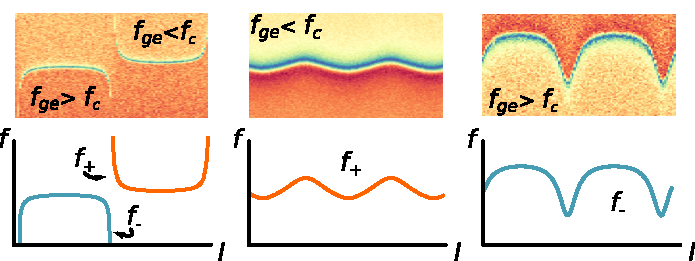
\includegraphics[width=.8\linewidth]{Pictures/detection}
	\caption{Желаемые результаты работы алгоритма при распознавании трех случаев однотоновой спектроскопии}
	\label{fig:detection}
\end{figure}

Таким образом, алгоритм должен распознавать на однотоновых спектрах указанные выше кривые \cite{filipp2011multimode}
\begin{align}
f_\pm(I) \equiv f_r(I) = \frac{f_c + f_{ge}(I)}{2} \pm \sqrt{g^2+(f_{ge}(I) - f_c)^2/4},\label{eq:f_r}
\end{align}
где $f_r(I) = f_c$ когда $g=0$, а $f_{ge}(I)$ выражается как
\begin{equation}
f_{ge}(I) = f_{ge}^{max} \left[\cos^2\left(\frac{\pi(I-I_{ss})}{\Pi}\right)+d^2 \sin^2 \left(\frac{\pi(I-I_{ss})}{\Pi}\right)\right]^\frac{1}{4}.
\label{eq:tr_spectrum}
\end{equation}
На \autoref{fig:detection} показано, как алгоритм должен интерпретировать однотоновые спектры в случаях, когда присутствуют или отсутствуют квазипересечения: в первом случае он должен аппроксимировать зависимость обеими кривыми одновременно, что значительно усложняет задачу; каждый из оставшихся двух случаев по отдельности представляет гораздо более простую задачу, но зато возникает дополнительная проблема выбора между двумя кривыми. В \autoref{tab:pars} для удобства собраны все 6 параметров модели с разъяснением их физического смысла.

Так как физическая модель известна, естественно попробовать вычислить её параметры на основе метода максимального правдоподобия (ММП, см. также Доп. \ref{sec:MLE}). Если считать, что экспериментально наблюдаемая частота резонатора распределяется нормально вокруг модели, этот метод сводится к глобальной оптимизации нелинейной задачи минимальных квадратов. Известно, что периодичность по параметрам (в нашем случае, таких два: $\Pi$ и $I_{ss}$) усложняет задачу, так как добавляет в функцию потерь большое количество ложных минимумов. К счастью, как будет показано ниже, можно устойчиво и достаточно точно определять начальные приближения для этих параметров независимым полуаналитическим методом. Другой проблемой является большая нелинейность модельной функции по другим параметром. Для борьбы с ней, а также с эффектами, вызванными разрывностью, применяется метод грубой силы для определения местонахождения оптимальной ``долины'' со склонами, гладкими достаточно для применения локального оптимизатора. 

\begin{table}
	\centering
	\small{\begin{tabular}{r c l}\toprule
			Пар. & Разм. & Значение\\\midrule 
			$f_c$ & Гц & собственная частота резонатора \\ 
			$g$ & Гц & константа взаимодействия кубита и резонатора \\
			$\Pi$ & A & период по току спектра трансмона \\
			$I_{ss}$ & A & положение верхней оптимальной точки по току \\
			$f_{ge}^\text{max}$ & Гц & частота трансмона в верхней оптимальной точке \\
			$d$ & & параметр асимметрии СКВИДа трансмона\\
			\bottomrule
	\end{tabular}}
	\caption{Параметры модели, их размерность и физический смысл.}
	\label{tab:pars}
\end{table}

\subsection{Предварительная обработка данных}

Наиболее трудным случаем является картина с квазипересечениями, поэтому будем рассматривать именно её. На \autoref{fig:antisubplots}~(а) изображена абсолютная величина пропускания через образец в зависимости от частоты $f_p$ (вертикальная ось) и тока в соленоиде, его окружающем. Пропускание выражается через соответствующий коэффициент комплексной матрицы рассеяния $S_{ij}$, где $i$ и $j$ -- номера выходного и входного микроволновых портов исследуемого устройства \cite{pozar2011microwave}. На образце, которое использовалось для получения данного графика, было два порта, поэтому изображается коэффициент $S_{21}$. Кроме модуля $S_{21}$ часто используется его комплексная фаза, особенно в случае, когда применяется резонатор, подсоединенный на отражение (если его внутренняя добротность велика, амплитуда отражения практически не будет меняться при прохождении через резонанс \cite{probst2015efficient}); в нашем же случае рассматривается резонатор шунтирующего типа (\foreignlanguage{english}{\textit{notch port}}, \cite{probst2015efficient}), который, являясь по сути узкополосным режекторным фильтром, дает глубокий и ясно видимый провал на АЧХ. Однако самым корректным методом является использование полной комплексной величины $S_{21}$, что мы и будем делать далее.


\begin{figure}
	\centering
	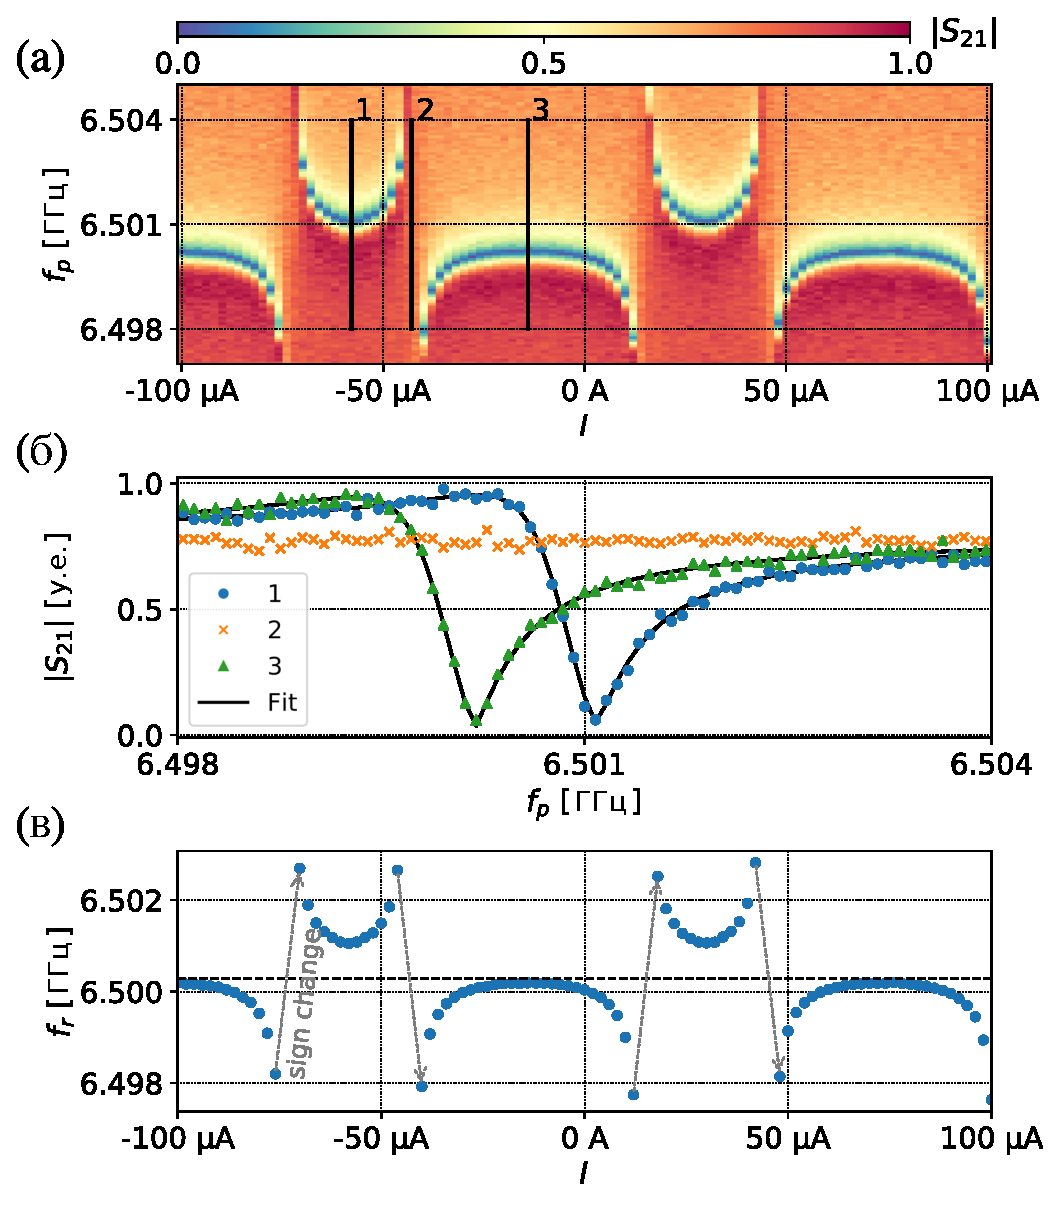
\includegraphics[width=0.7\linewidth]{Pictures/anti_subplots}
	\caption{\textbf{(а)} Исходная тепловая карта модуля коэффициента матрицы рассеяния $|S_{21}|$ в зависимости от тока и частоты векторного анализатора $f_p$. \textbf{(б)} Срезы пропускания с (а), на 1 и 3 резонансный пик присутствует и аппроксимирован аналитической кривой, а на 2 наблюдается плато. \textbf{(в)} Извлеченная резонансная частота $f_r(I)$ (синие точки) и средняя по току частота (черная прерывистая линия). Серые стрелки показывают точки, в которых происходит смена знака функции $f_r - \langle f_r\rangle_I$.}
	\label{fig:antisubplots}
\end{figure}

На \autoref{fig:antisubplots}~(а) невооруженным глазом видна периодичность перемещений резонансного провала в направлении оси абсцисс. С учетом того, что моделью являются одномерные кривые, нет необходимости работать со всем изображением. Первым шагом в обработке будет выделение непосредственно резонансной частоты при помощи уже существующей библиотеки \foreignlanguage{english}{\textit{circlefit}} \cite{probst2015efficient}. Если рассмотреть вертикальные срезы тепловой карты (АЧХ при фиксированном токе), обозначенные линиями 1, 2 и 3, то получатся графики на \autoref{fig:antisubplots}~(б); видно, что в то время как кривые 1 и 3 показывают резонанс, срез 2 является плоским. Соответственно, для применения алгоритма библиотеки \foreignlanguage{english}{\textit{circlefit}} требуется предварительно отсеять плоские участки при помощи порогового условия на изменение амплитуды $S_{21}$ (см. \cite{fedorov2021github}, файл \foreignlanguage{english}{lib2/fulaut/AnticrossingOracle.py}). Участки, содержащие резонанс, аппроксимируются моделью для шунтирующего резонатора:
\begin{equation}
	S_{21}^\text{notch}(f_p) = ae^{i\alpha}e^{2\pi if_p\tau} \left[1-\frac{Q_l/Q_e'}{1+2iQ_l(f_p/f_r-1)}\right],
	\label{eq:res_S21_probst}
\end{equation}
где $a$ обозначает полную аттенюацию (усиление) в измерительном тракте, $\alpha$ -- это постоянный сдвиг фаз в нем, не зависящий от частоты, $\tau$ -- задержка распространения сигнала из-за конечной длины проводов вдали от резонанса; $Q_l, Q_e^\prime$ -- это стандартная полная (нагруженная) добротность и комплексная \cite{khalil2012} внешняя добротность резонатора, а $f_r$ -- резонансная частота. Как можно видеть, в качестве модели используется комплекснозначная функция, поэтому и амплитуда, и фаза оказываются учтенными. Библиотека \foreignlanguage{english}{\textit{circlefit}} последовательно устанавливает значения этих параметров, на окончательном шаге используя аналитическую формулу для определения положения и размеров окружности, образуемой точками на комплексной плоскости зависимостью \eqref{eq:res_S21_probst} по методу наименьших квадратов (практически все линейные резонансные системы дают именно такую форму параметрической кривой, подробности работы алгоритма можно найти в оригинальной работе \cite{probst2015efficient}). На \autoref{fig:antisubplots}~(б) непрерывные черные кривые показывают модуль правой части \eqref{eq:res_S21_probst}, построенной для найденных оптимальных значений параметров. Для краткости мы не приводим полных комплексных графиков, однако заверяем читателя, что совпадение параметрических кривых также оказывается превосходным.

На \autoref{fig:antisubplots}~(в) построен график извлеченных таким образом значений $f_r$. Для некоторых точек по току данные отсутствуют, что неизбежно в силу отсутствия там резонансного провала. Помимо этого, черной прерывистой линией мы показываем на этом графике усредненную частоту $\langle f_r\rangle_I$, которая будет использоваться в качестве начального приближения для $f_c$, а также в промежуточном алгоритме извлечения фазы и периода в зависимости $f_r(I)$, о котором мы будем говорить ниже. Здесь стоит также обсудить закон распределения $f_r(I)$, который ранее предполагался гауссовским. Стоит отметить, что для нелинейной задачи ММП вопрос распределения статистической функции оценки, коей является извлекаемая случайная величина $f_r$, является, фактически нерешаемым аналитически. Единственный способ установить его -- эмпирический, заключающийся в многократном запуске алгоритма и построении гистограммы получающихся значений. Автор не выполнял этой процедуры для библиотеки \foreignlanguage{english}{\textit{circlefit}}; не выполнялась она и в оригинальной работе. Однако в дальнейшем все же весьма удобно считать распределение $f_r$ нормальным или близким к нормальному для аналитического определения предела Рао-Крамера для дисперсии определяемых по ММП параметров полной модели \eqref{eq:f_r}.

\subsection{Определение периода $\Pi$ и положения оптимального тока $I_{ss}$}

Как говорилось ранее, одна из проблем для поиска глобального максимума функции правдоподобия, или глобального минимума суммы квадратов разностей модели и данных, -- это периодичность данных. Так как фаза сигнала также неизвестна, в функции потерь образуется большое количество локальных минимумов, которые мешают продвижению итерационных алгоритмов. Другими словами, включение параметров $\Pi$ и $I_{ss}$ в задачу оптимизации делает её практически неразрешимой стандартными методами: локальные алгоритмы не могут сдвинуться от начальных параметров и ``застревают'', в чем автор многократно убеждался, пытаясь поначалу использовать ``в лоб'' стандартные методы из библиотеки \foreignlanguage{english}{scipy.optimize}; оптимизация по методу грубой силы оказывается невозможной, так как добавление в сетку еще двух параметров с разрешением хотя бы в 50 точек замедляет расчет в 2500 раз. Более того, алгоритму заранее неизвестно, в каких пределах строить сетку для параметра $\Pi$, что делает грубый поиск принципиально неудобным подходом. Таким образом, было бы весьма удобно получить значения периода и фазы сигнала, вовсе не используя полную модель. При отсутствии шума алгоритмическое решение было бы тривиальным: достаточно было бы рассмотреть функцию $\Delta f_r = f_r-\langle f_r \rangle_{I}$ и найти точки, в которых она меняет знак. Минимальное расстояние между одинаковыми сменами знака дало бы период, а середина одного из двух отрезков между противоположными сменами знака дала бы оптимальную точку по току $I_{ss}$. Однако, как показывает практика, присутствие даже малейшего шума делает этот метод неустойчивым и полностью непригодным. В этой связи автором был предложен подход, нечувствительный к локальным возмущениям в данных эксперимента.

\begin{figure}[t]
	\centering
	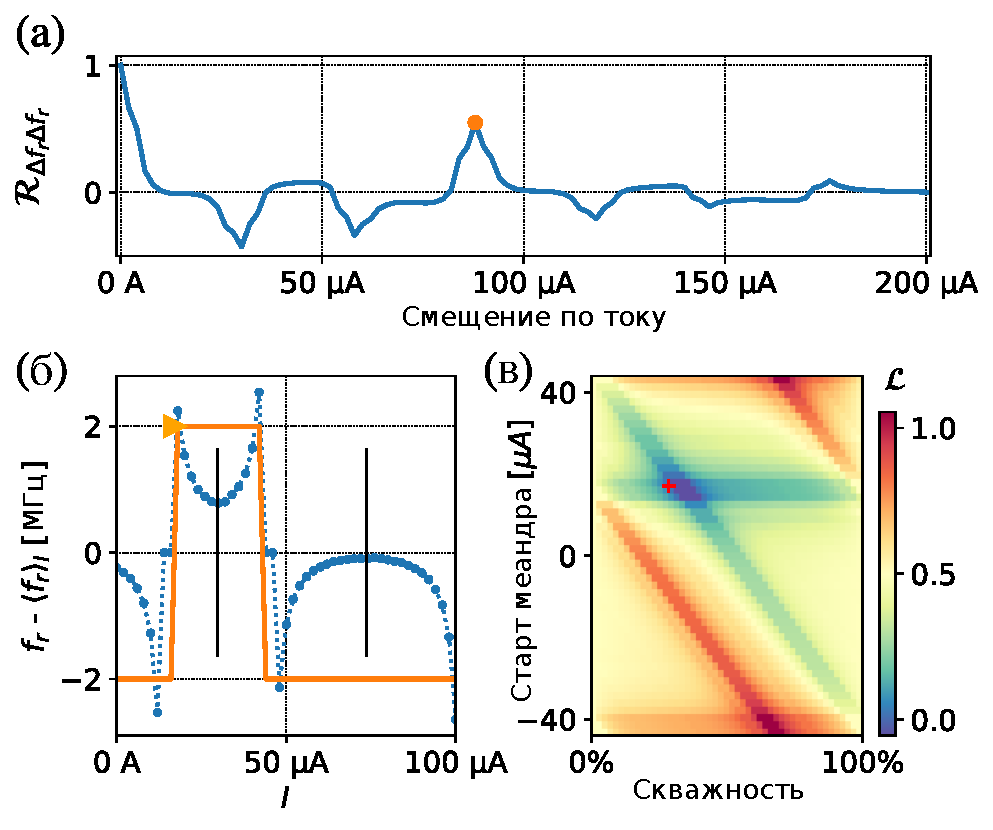
\includegraphics[width=0.7\linewidth]{Pictures/per_phase}
	\caption{Иллюстрация к процедуре извлечения $\Pi$ и $I_{ss}$. \textbf{(а)} Автокорреляционная функция в зависимости от смещения по току, показывающая хорошо видный максимум на 88 $\mu$А (оранжевая точка). \textbf{(б)} Построение для определения $I_{ss}$; $\Delta f_r = f_r-\langle f_r \rangle_{I}$ (синяя) сворачивается с прямоугольным сигналом (оранжевый, начало периода отмечено треугольным маркером). Черные вертикальные линии отмечают предположительные положения оптимальной точки. \textbf{(в)} Функция потерь (нормированная) для свертки с прямоугольным сигналом; красный крест показывает параметры, выбранные для построения меандра на (б).}
	\label{fig:perphase}
\end{figure}

Очевидным методом для определения периода и фазы сигнала (в нашем случае фаза эквивалентна положению $I_{ss}$) является преобразование Фурье. К цифровым данным применяется быстрое преобразование Фурье (БПФ), и самый высокий по абсолютной величине его пик даст амплитуду и фазу наиболее существенной периодической компоненты разложения сигнала. БПФ хорошо подходит для непрерывных кривых, но оказывается неустойчив при анализе квазипересечений: спектр оказывается слишком сложным, а истинный пик -- часто не самым высоким. Также БПФ испытывает проблемы с точностью при наличии всего нескольких периодов. Более подходящим методом для поиска периода в дискретном наборе данных $\{y_i\}$ является автокорреляционная функция $\mathcal{R}_{y y}(l) = \sum_n y_n y_{n-l}$. Положение её самого высокого локального максимума (за исключением $l=0$) дает искомый период сигнала \cite{parthasarathy2006}. Это утверждение верно только для наборов данных с нулевым средним значением, поэтому удобно использовать для расчета автокорреляции уже введенную ранее функцию $\Delta f_r = f_r-\langle f_r \rangle_{I}$, которая имеет тот же период и фазу, что и исходная. Для неё $\mathcal{R}_{\Delta f_r \Delta f_r}(\Delta I)$ в зависимости от смещения по току $\Delta I$ изображена на \autoref{fig:perphase}~(а). Здесь $\Delta I$ при вычислении свертки пробегает те же значения, что и $I$ на исходном графике \autoref{fig:antisubplots}~(в). Это означает, что данные при вычислении дополняются нулями на краях для всех смещений, кроме $\Delta I = 0$, поэтому мы получаем всё уменьшающиеся корреляционные пики в точках $\Pi,\ 2\Pi,$ и т.д. Оранжевой точкой мы отмечаем самый высокий пик на 88 $\mu$А. Как видно, он очень яркий, и легко определяется на фоне остальных. Также можно заметить маленький пик двойного периода на 176 $\mu$А. Отметим, что автокорреляционная функция не идеально гладкая, как была бы в случае отсутствия квазипересечений; этот эффект вызван отсутствующими участками в данных из-за плато на \autoref{fig:antisubplots}. Чтобы положение пика $\mathcal{R}_{\Delta f_r \Delta f_r}$ было верным, необходимо было заполнить эти участки нулями (они хорошо заметны на \autoref{fig:perphase}~(б), синие точки).


Недостатком метода с автокорреляционной функцией является то, что она не может дать никакой информации о фазе сигнала, то есть о положении оптимальной точки. Поэтому требуется ``дооснастить'' наш алгоритм еще одной процедурой для вычисления $I_{ss}$. Заключается она в определении глобального максимума несмещенной свертки $\mathcal{R}_{\Delta f_r S}(0)$ между $\Delta f_r(I)$ и прямоугольным сигналом $S(I, \Pi, \phi, D)$, имеющим такой же период $\Pi$ (уже известный алгоритму) и требующие определения фазу $\phi$ и скважность $D$ (отношение длин его верхнего и нижнего горизонтальных промежутков). Верхнее и нижнее значения должны быть противоположны по знаку, а по модулю могут быть произвольны, так как это не повлияет на положение искомого оптимума. На \autoref{fig:perphase}~(б) оранжевым цветом изображен правильно наложенный прямоугольный сигнал, максимизирующий значение свертки. Его фаза (в $\mu$А) обозначает токовую координату первой точки после переднего фронта и отмечена треугольником. Основа идеи этого подхода лежит во всё той же попытке определения положения смены знаков, однако теперь с гораздо большей устойчивостью. Понятно, что $\mathcal{R}_{\Delta f_r S}(0) = \sum_I \Delta f_r(I) \cdot S(I) $ увеличивает свое значение, если $\Delta f_r$ и $S$ оказываются одного знака для определенного $I$. Поэтому комбинация $\phi, D$, которая обеспечивает максимальное количество точек, где $f_r(I)\cdot S(I)>0$, т.е. правильно определяет положения смены знаков, доставляет максимум и $\mathcal{R}_{\Delta f_r S}(0)$. Так как период уже зафиксирован, процедура будет работать даже в случае, если $\langle f_r \rangle_{I}$ пересечет одну из ветвей квазипересечений.

Оптимальные значения для $\phi$ и $D$ находятся при помощи метода грубой силы. Функция потерь $\mathcal{L} = - \mathcal{R}_{\Delta f_r S}(0)$ рассчитывается на сетке размером 50$\times$50 и затем возвращаются координаты минимального её значения. Благодаря наличию вполне ясных ограничений на $\phi \in [-\Pi/2,\ \Pi/2)$ и $D\in [0,1]$ этот метод работает быстро и стабильно. Топографию функции потерь для квазипересечений достаточно проста, как можно видеть из \autoref{fig:perphase}~(в). Единственная особенность её заключается в том, что из-за наличия нулевых значений, о которых ранее говорилось, точек, отвечающих минимальному значению, оказывается несколько; однако любая из них подойдет для последующего использования.

После определения $\Pi,\ \phi$ и $D$ можно, наконец, расчитать положение $I_{ss}$. Для квазипересечений
\begin{equation}
	I_{ss} = \phi + \Pi (1+D)/2.
\end{equation}
Для непрерывных зависимостей, наоборот,
\begin{equation}
	I_{ss} = \phi + \Pi D/2.
\end{equation}
Так как пока что алгоритм не выяснил, какой тип картины ему представлен, ему потребуется применить некоторый эвристический критерий, чтобы угадать, какое из двух уравнений применять. Если шум не слишком большой, в качестве такого критерия может быть выбрано значение максимального по модулю дискретного дифференциала зависимости частоты от тока $\max_{i>0} | f_{r,i} - f_{r,i-1} |$ в сравнении с размахом данных $\max_{i,j} |f_{r,i} - f_{r,j}|$. Для квазипересечений эти две величины будут близки, а для непрерывных зависимостей сильно отличны друг от друга. Однако в случае сильной зашумленности данных, которая определяется в алгоритме через медианную дисперсию дискретного дифференциала в сравнении с размахом данных, этот индикатор может давать неправильный ответ, а значит придется проверять оба значения $I_{ss}$ и выбрать из них то, которое даст меньшую ошибку при аппроксимации полной модели.

\subsection{Аппроксимация полной модели}

После того, как выполнены шаги, рассмотренные выше, можно приступать к методу максимального правдоподобия для полной модели \eqref{eq:f_r}. Как уже обсуждалось, мы используем сначала метод грубой силы, а в качестве локального оптимизатора, запускающегося с найденным результатом в качестве начального приближения, выбираем сипмлекс-метод Нелдера-Мида \cite{nelder1965}. Для обоих методов используется общая функция потерь, основанная на ММП (еще раз отметим необходимость предположения о нормальном распределении $f_r$ вокруг модели). Для известного диапазона частот $\Delta f_p$ (\autoref{fig:antisubplots}~(a), вся ось ординат) и множества $N$ извлеченных точек $\{p_i\} = \{(I_i, f_{r,i})\}$ мы вычисляем функцию потерь как
\begin{align}
\mathcal{L} &= \sum_{i=1}^N [f_{r,i} - \mathcal{M}(I_i,\ \Pi, \ I_{ss},\ f_c,\ g,\ f_{ge}^{max},\ d)]^2,\label{eq:loss}\\
\mathcal{M} &= \begin{cases}
f_+,\  |f_+ - f_c|< \Delta f_p/2 \\
f_-,\ \text{otherwise}, \label{eq:cond}
\end{cases}
\end{align}
где, как и в разделе \ref{sec:sts_theory},
\[
f_{\pm} = f_{\pm}(I_i,\ \Pi,\ I_{ss},\ \ f_c,\ g,\ f_{ge}^{max},\ d).
\]
Условие \eqref{eq:cond} означает, что мы выбираем только те значения модели, которые лежат внутри диапазона шириной $\Delta f_p$ вокруг $f_c$. Это обеспечивает, во-первых, что в оптимуме мы не получим модельных точек, попадающих за пределы экспериментальной области, и, во-вторых, что у нас будет не более одного значения частоты для каждого значения тока (иначе модель будет многозначной функцией).

\begin{figure}[t!]
	\centering
	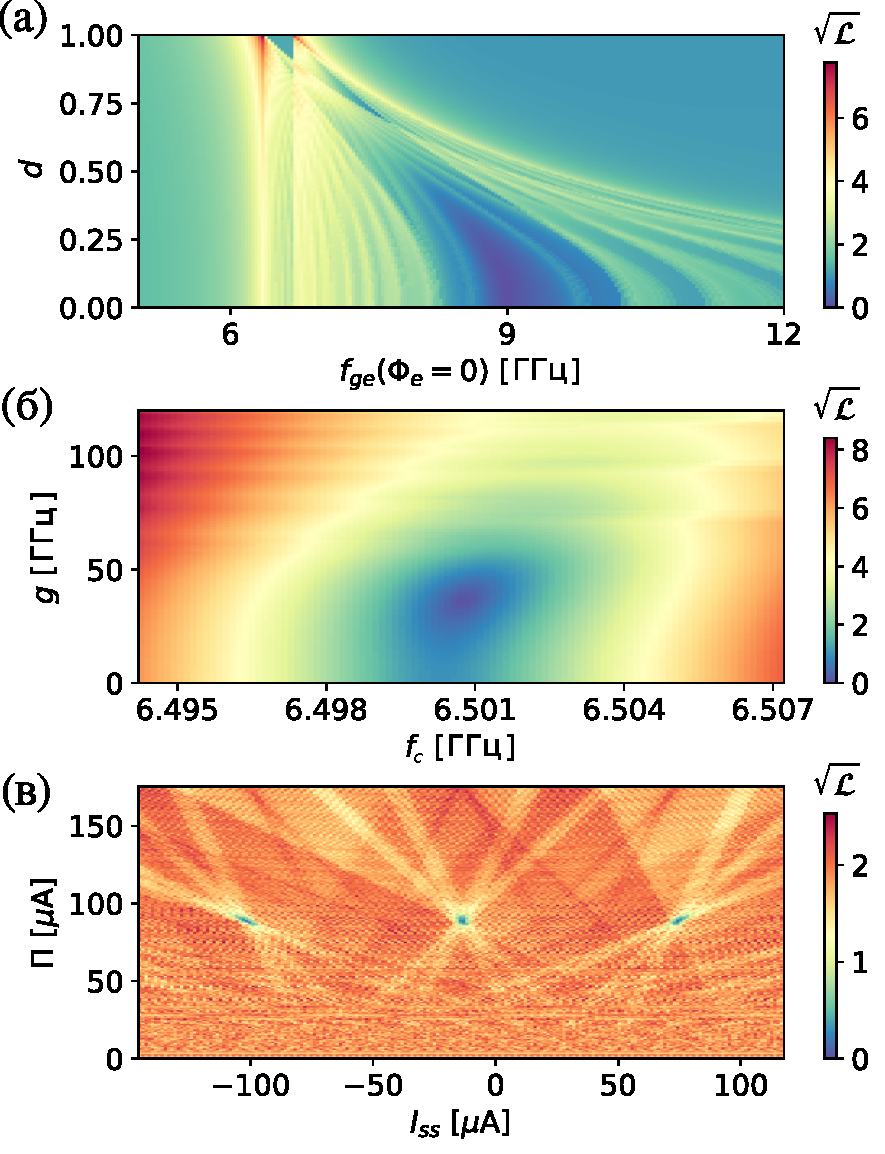
\includegraphics[width=0.6\linewidth]{Pictures/loss1}
	\caption{Двумерные сечения функции потерь \eqref{eq:loss} для данных из \autoref{fig:antisubplots} в окрестности оптимума. Цветом показана среднеквадратичная ошибка, приходящаяся на точку, $\sqrt\mathcal{L}$, в МГц. \textbf{(a)} $f_{ge}^\text{max}$ и $d$ изменяются, остальные параметры в оптимуме. Оптимальная ``долина'' вокруг глобального минимума находится вблизи 9 ГГц; можно видеть также большое число ложных минимумов вокруг неё. \textbf{(б)} $g$ и $f_c$ изменяются. Для этих параметров функция потерь рядом с глобальным минимумом устроена достаточно просто. \textbf{(в)} $\Pi$ и $I_{ss}$ изменяются. Как видно, для этой пары параметров функция потерь устроена очень сложно, а размеры оптимальной долины оказываются чрезвычайно малыми.}
	\label{fig:loss1}
\end{figure}

Чтобы обосновать использование именно такой схемы оптимизации, мы строим на \autoref{fig:loss1} несколько тепловых карт, показывающих срезы функции потерь при фиксированных значениях четырех из шести параметров. Даже из этих трех графиков, показывающих только часть многомерного пространства, очевидно, что функция потерь устроена весьма сложным образом. Она не только содержит большое количество ложных минимумов, но к тому же имеет скачки, обусловленные \eqref{eq:cond}, что сразу исключает применение градиентных методов. Параметры $f_{ge}^\text{max}$ и $d$ представляют существенную трудность в силу наличия большого числа локальных минимумов и малой крутизны склонов. Напротив, $f_c$ достаточно легко может быть найдена; однако, следует учитывать, что это так только тогда, когда фиксированные параметры близки к оптимальным. Наконец, период и положение оптимальной точки представляют наибольшую трудность и иллюстрируют необходимость использования полуаналитического метода, приводящего алгоритм сразу в оптимальную точку по этой паре. Здесь также отчетливо видны полосы, возникающие из-за того, что вокруг разрывов модельной функции в силу дискретности шага по току точки то попадают в окно \eqref{eq:cond}, то оказываются за его пределами.

Алгоритм грубой силы работает на сетке, параметры которой указаны в \autoref{tab:grid}. Диапазоны выбираются в согласии с обычно используемыми в наших лабораториях параметрами дизайна образцов, а число шагов устанавливается эмпирическим путем как минимальное для надежной работы алгоритма. Как видно, для $f_c$ достаточно всего трех точек, в то время как для $f_{ge}^\text{max}$ требуется значительный перебор. Теоретически, число шагов может постепенно увеличиваться самим алгоритмом во время выполнения до тех пор, пока результат не перестанет меняться (адаптивное разбиение гиперпространства, см. например \cite{Nijholt2019}). После грубого определения положения оптимального региона запускается локальный оптимизатор по всем шести параметрам.

\begin{table}
	\centering
		\small{\begin{tabular}{lll} \toprule
			Параметр & Диапазон & Число шагов \\ 
			\midrule
			$f_c$ & $\langle f_r \rangle_{I} \pm 1$ МГц & 3\\ 
			$g$ & 20 -- 40 МГц & 5\\
			$f_{ge}^\text{max}$ &  4 -- 12 ГГц & 80 \\
			$d$& 0 -- 0.9 & 9\\
			\bottomrule
		\end{tabular} }
	\caption{Спецификация сетки для полного перебора методом грубой силы.}
	\label{tab:grid}
\end{table}

\subsection{Демонстрация работы алгоритма}

Описанный алгоритм был реализован автором на языке \foreignlanguage{english}{\textit{Python}} с использованием функций библиотеки \foreignlanguage{english}{\textit{scipy}}. Рассмотрим его работу на всех трех случаях взаимного расположения кубита и резонатора. Полученные результаты представлены на \autoref{fig:fitcases}, и в дальнейшем мы будем называть каждый из случаев как (a), (б) или (в), соответственно.

\begin{figure}
	\centering
	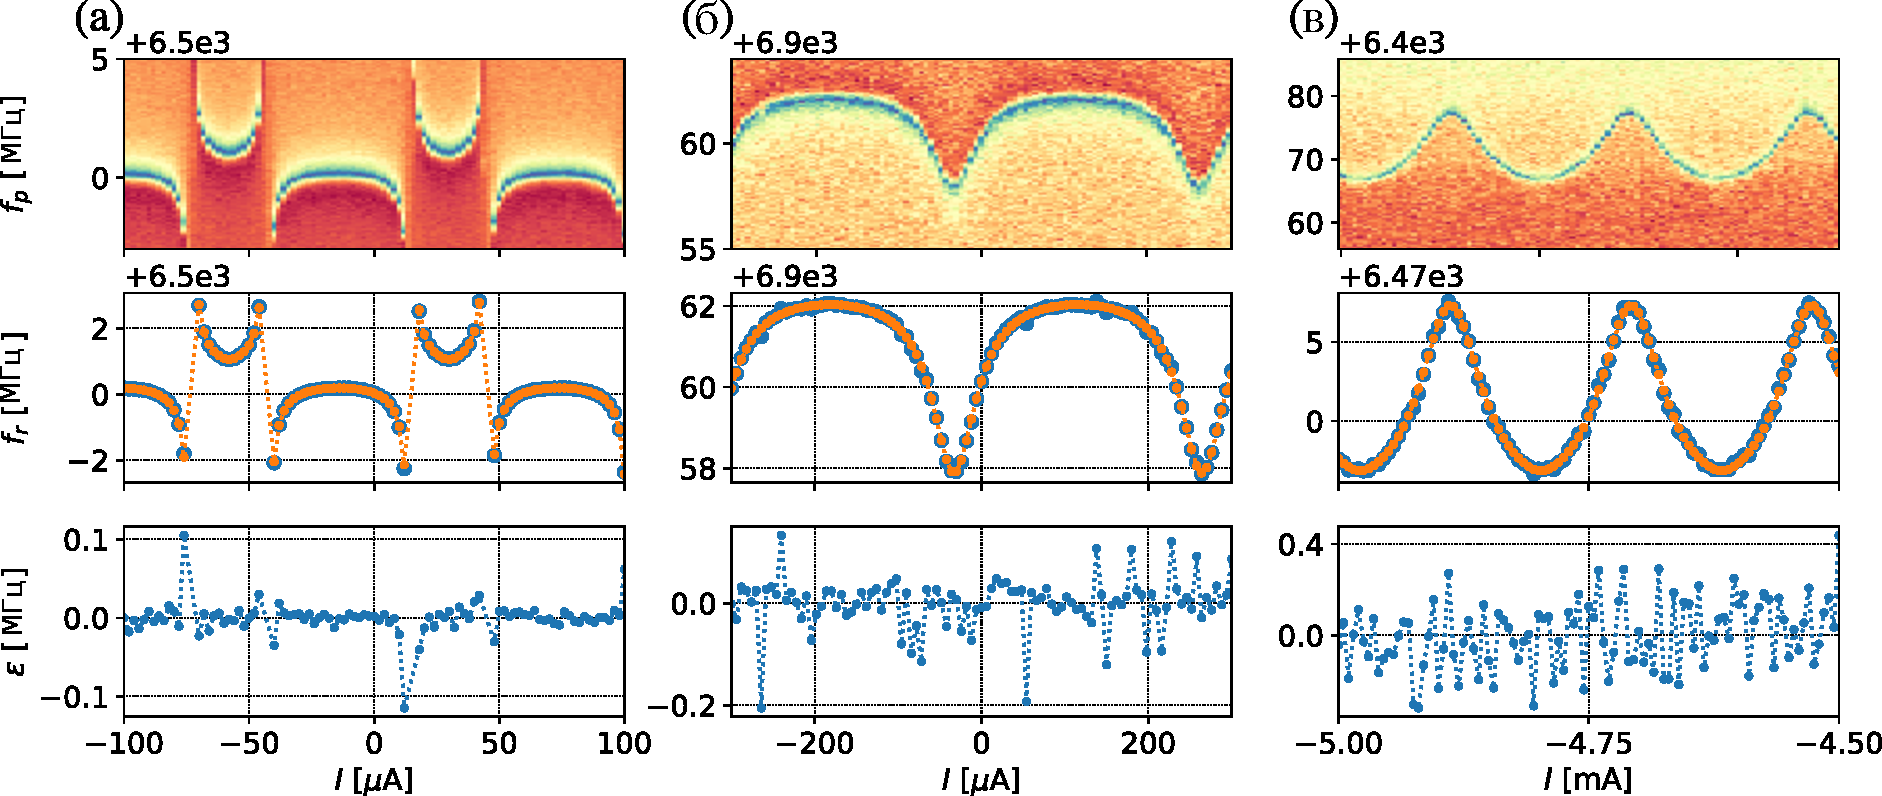
\includegraphics[width=1\linewidth]{Pictures/fit_cases}
	\caption{Результаты работы алгоритма на трех экспериментальных наборах данных, выбранных в качестве примера из нашей базы данных. В верхнем ряду показаны исходные изображения. В среднем ряду построены данные (синие точки) и аппроксимированная модель (соединенные оранжевые точки). В нижнем ряду показаны разности между моделью и данными. Среднеквадратичное отклонение на точку равно: \textbf{(а)} 30 кГц для квазипересечения; \textbf{(б)} 60 кГц для кубита над резонатором; \textbf{(в)} 150 кГц для кубита под резонатором.}
	\label{fig:fitcases}
\end{figure}

\begin{table*}
	\centering
		\renewcommand{\arraystretch}{1.2}
		\setlength{\tabcolsep}{4pt}
		\footnotesize{
		
		\hspace*{-0cm}\begin{tabular}{*{13}{l}} \toprule
			\multirow{2}{*}{\textbf{Параметр}} & 
			\multicolumn{4}{l}{\textbf{(a)}} & 
			\multicolumn{4}{l}{\textbf{(б)}} & \multicolumn{4}{l}{\textbf{(в)}}\\
			& Пер. & Н-М & $\min \sigma$ & ДТС  & Пер. & Н-М & $\min \sigma$ & ДТС  & Пер. & Н-М & $\min \sigma$ & ДТС  \\
			\hline
			$f_c$, ГГц &6.5003 & 6.5007 &  4$\times 10^{-6}$ & n/a & 6.962 & 6.9631 & 1.6 $\times 10^{-4}$  & n/a &  6.47 & 6.465& 2$\times 10^{-4}$ & n/a\\ 
			$g$, ГГц & 24 & 35.8 & 0.17 & n/a & 36 & 64.9 & 15 & n/a & 36 & 86.1& 1 &n/a\\
			$f_{ge}^\text{max}$, ГГц & 8 &\textbf{8.97} & 0.013 & \textbf{9.04} &10.3& \textbf{11.3}& 1.35 & \textbf{9.08}& 6.3& \textbf{5.89}&0.01&\textbf{5.9}\\
			$d$ &0.5& \textbf{0.09}& 0.013& \textbf{0.13} &0.5&\textbf{0.49} &0.07&\textbf{0.6}&0.1& \textbf{0.25} & 0.05 &\textbf{0.3} \\\hline
			Ошибка, кГц & 251 & 20 && &338& 51 & & &2038& 149&&\\
			\bottomrule
		\end{tabular} }
	\caption{Анализ оптимальных параметров, найденных для трех случаев из \autoref{fig:fitcases} после грубого поиска полным перебором и после алгоритма Нелдера-Мида. Колонки $\min \sigma$ обозначают нижние границы дисперсии ММП-оценок, полученные из информационной матрицы Фишера в оптимуме.}
	\label{tab:sts_results}
\end{table*}


В \autoref{tab:sts_results} анализируются результаты аппроксимации для обозначенных трех случаев. Сравнивая значения параметров, полученные после грубого поиска и после симплекс-метода, можно увидеть, что процедура работает, как ожидалось: полный перебор дает достаточно хорошее начальное приближение для алгоритма Нелдера-Мида, а последний затем успешно находит гораздо более точный ответ, который достигается, в основном, за счет более качественного определения параметра $f_c$, на который в сетке грубого поиска дается всего три точки. Изменение её значений ведет, в свою очередь, к значительным смещениям оптимальных $g,\ f_{ge}^\text{max},\ d$.

Вполне ожидаемо, что оптимальные значения для параметров кубита и силы связи могут иметь некоторую ошибку по сравнению с истинными значениями. Например, в случае (б) предсказанная максимальная частота кубита $f_{ge}^\text{max}$ более чем на 2 ГГц отличается от значения, полученного для того же образца при помощи двухтоновой спектроскопии. В случаях (а) и (в) отличия этого параметра гораздо меньше (10-70 МГц), зато асимметрия оказывается определена с ошибкой порядка 10\%. Ошибки при определении параметров кубитов могут быть объяснены, в частности, малой чувствительностью частоты резонатора к смещению частоты кубита, когда они сильно отстроены друг от друга; с другой стороны, между параметрами наблюдаются сильные корреляции (меняя два параметра одновременно, можно получить гораздо меньшее изменение функции правдоподобия, чем если бы каждый по отдельности изменялся на ту же величину).

Для того, чтобы оценить погрешности определения параметров, мы прибегаем к аналитическому вычислению информационной матрицы Фишера (см. Доп. \ref{sec:MLE}) в оптимуме. В \autoref{tab:sts_results} колонки $\min\sigma$ показывают корень из соответствующего предела Рао-Крамера для дисперсии ММП-оценки каждого из параметров. Из таблицы видно, что высокие $\min\sigma$ предсказывают бóльшую ошибку по сравнению с данными ДТС. Дополнительно автором проводился анализ главных компонент матрицы Гесса, который позволяет определить наименее жестко определенные комбинации параметров (направления больших полуосей многомерного эллипса, образуемого постоянным значением функции потерь вблизи оптимума). Выяснилось, что таковыми является вектор с компонентами $f_c,\ g,\ f_{ge}^\text{max},\ d$ и на порядок более жестко определенная пара $\Pi$ и $I_{ss}$. чтобы уменьшить корреляции, можно использовать другую параметризацию, например, заменив $d$ и $f_{ge}^\text{max}$ на $E_{J}^\text{max}$ и $E_J^\text{min}$, которые не будут скоррелированы между собой; автором, однако, такой подход не тестировался, так как на текущий момент достигнутая точность оказалась на практике достаточной. Также стоит отметить, что точность определения частоты кубита значительно увеличивается, если задать заранее известный из дизайна или эмпирически параметр связи $g$. В разработанном авторе коде фиксировать один или несколько параметров перед запуском оптимизации можно, передав в конструктор объекта \foreignlanguage{english}{\textit{AnticrossingOracle}} соответствующий словарь, или же, на более высоком уровне, записав его в файл конфигурации параметров эксперимента.

Так как в реальных условиях высокое отношение сигнал/шум (ОСШ) во входных данных не гарантировано (оно зависит от мощности сигнала, а также от общей аттенюации и усиления в измерительном тракте, и от свойств конкретного образца), автором проводилось его стресс-тестирование на устойчивость путем добавления искусственно сгенерированного шума к данным перед запуском алгоритма. Так как исходные экспериментальные данные уже содержали какой-то шум, была введена общая для всех шкала ОСШ. Сама величина ОСШ определялась как обычно делается для данных по измерениям сверхпроводящих резонаторов \cite{probst2015efficient}: раз S-параметр лежит на окружности в комплексной плоскости, логично выбрать в качестве амплитуды сигнала его радиус. Тогда для комплексного шума вида $(\xi_1 + i\xi_2)/\sqrt{2}$, где $\xi_1,\ \xi_2$ распределены нормально с нулевым средним и среднеквадратическим отклонением (СО) $\sigma$ ОСШ определяется нами как
\begin{equation}
r/\sigma = r/\sqrt{\sigma_0^2+\sigma_1^2},
\label{eq:SNR}
\end{equation}
где $\sigma_0$ -- это оригинальное СО самих данных, а $\sigma_1$ относится к добавленному шуму. Очевидно, что в такой шкале ОСШ не может превышать $r/\sigma_0$.

Установив общую шкалу, мы тестировали алгоритм, добавляя нормальный шум с постепенно увеличивающейся дисперсией $\sigma_1^2$. Для каждого значения дисперсии проводилось 50 запусков и строилась гистограмма для каждого из параметров. Полученные в результате такого эксперимента графики изображены на \autoref{fig:noisetest}, где значения оси абсцисс графиков вычислялись по формуле \eqref{eq:SNR} ($r/\sigma_0$ указаны в подписи). Как видно, алгоритм стабилен начиная с ОСШ $\approx 2$ и достигает практически максимальной своей точности при ОСШ $\approx 3$. Стоит отметить, что в случаях (б) и (в) оригинальный ОСШ достаточно близок к добавленному, поэтому разброс оптимальных параметров был бы большим, если бы весь шум был сгенерирован искусственно. Стабильность алгоритма определяется, главным образом, стабильностью аппроксимации резонатора на шаге предварительной обработки данных.

\begin{figure}
	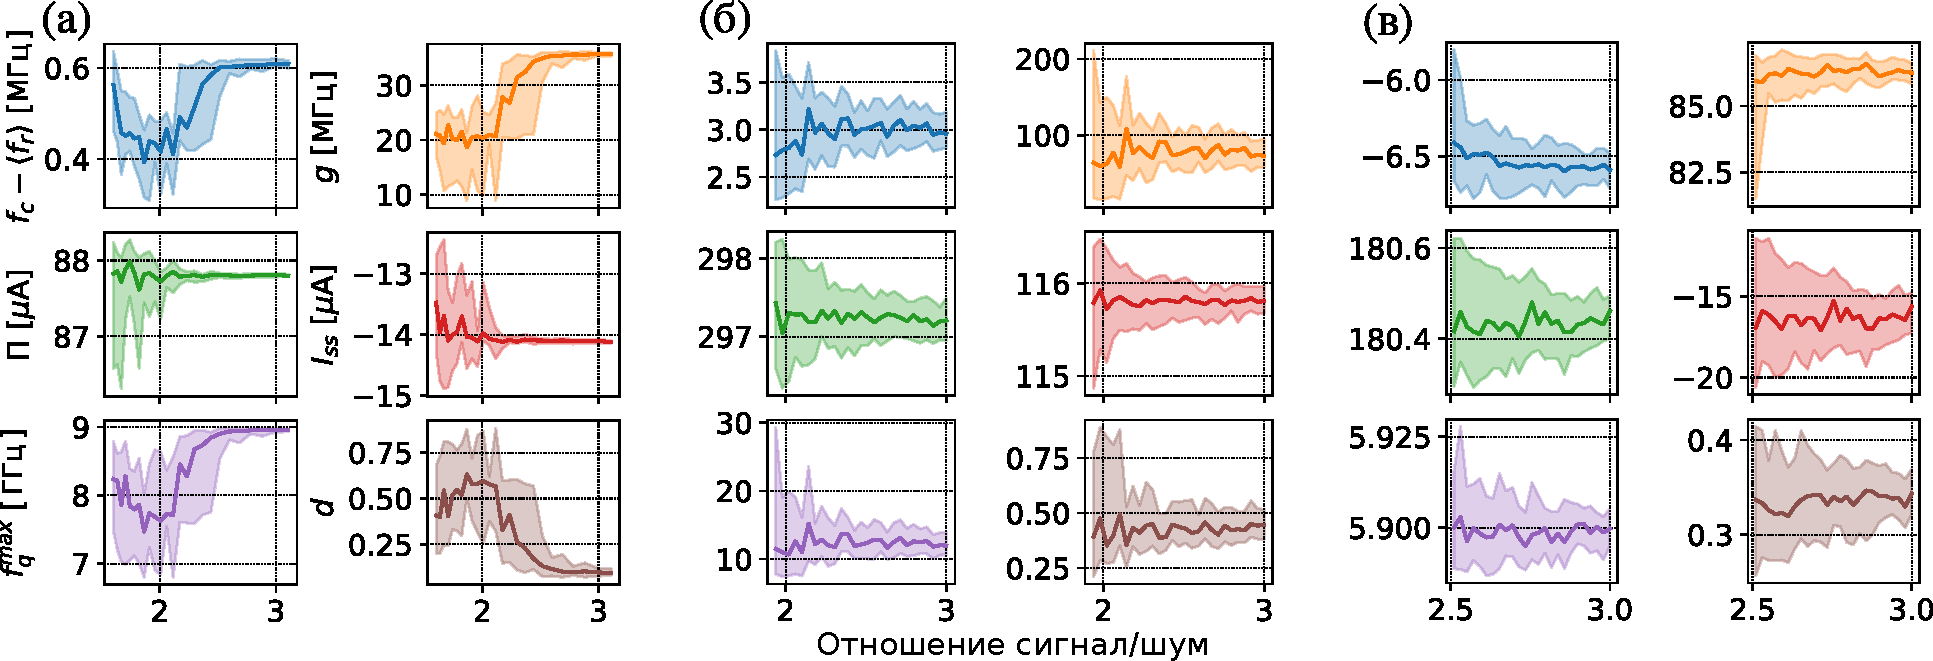
\includegraphics[width=1\linewidth]{Pictures/noise_test}
	\caption{Поведение алгоритма на данных из \autoref{fig:fitcases} с добавлением гауссового шума различной мощности, т.е. с искусственно ухудшенным отношением сигнал/шум (ОСШ). Закрашенные области показывают границы 25-го и 75-го процентилей по 50 запускам алгоритма с различными реализациями добавленного шума, сплошными линиями показано медианное значение. \textbf{(а)} Сигнал-шум в исходных данных составляет 19. Алгоритм точен начиная с ОСШ $=2.5$ (намного ниже оригинального) и устойчив при ОСШ $>1.5$. \textbf{(б)} Исходное ОСШ $=4.7$. Частота и асимметрия кубит не могут быть точно определены, но алгоритм устойчив до ОСШ $>2$. \textbf{(в)} Исходное ОСШ $=3.14$. Алгоритм точен при ОСШ $>2.5$, за исключением определения параметра $d$.}
	\label{fig:noisetest}
\end{figure}

 
В заключение раздела обсудим производительность алгоритма. Автором проводились тесты на двух машинах: на ноутбуке с Intel i5-3337U @ 2.5 ГГц и на компьютере с более современным Intel i7-7700. Время выполнения в первом случае для данных из (а) составляло около 7 с, в то время как во втором около 2 с. Самым затратным является первый шаг по предварительной обработке данных с помощью библиотеки \foreignlanguage{english}{\textit{circlefit}} (2.7 с, основное время тратится в итеративных калибровочных оптимизациях), затем идут грубый перебор и симплекс-метод, где основной трудностью является вычисление квадратных корней в модели \eqref{eq:f_r}. Для практических применений производительность достаточна, так как алгоритм работает гораздо быстрее, чем обработка в ручном режиме, не вносит ошибок, и занимает не слишком большое время по сравнению с выполнением самого измерения (порядка 20 секунд). В дальнейшем можно увеличивать производительность, например, отказавшись от библиотеки \foreignlanguage{english}{\textit{circlefit}} и используя более разумный перебор в методе грубой силы.

\begin{table}
	\centering
	\small{
		\begin{tabular}{llllll}\toprule
			&Извл. $f_r$& $\Pi$, $I_{ss}$ & Пер. &Н-М &
			\textbf{Итог}\\\midrule
			\textbf{Время}, s& 2.72& 0.3&2.79&1.37&7.34\\
			\textbf{Доля}, \% & 37 &4 &38 &18 &100\\
			\bottomrule
	\end{tabular}}
 \caption{Время выполнения алгоритма на двухъядерном процессоре i5-5337U с частотой 2.5 ГГц для случая (a). Дольше всего работают первый шаг, извлекающий частоту резонатора, а также полный перебор.}
 \label{tab:performance}
\end{table}

\subsection{Заключение}

	В данном разделе был описан предложенный автором алгоритм автоматической обработки и распознавания результатов однотоновой спектроскопии систем квантовой электродинамики цепей. Для определения параметров физической модели использовался метод максимального правдоподобия. Было показано, что можно достаточно точно оценивать параметры кубита по поведению частоты резонатора в зависимости от магнитного потока, управляющего частотой кубита, с ним связанного, для любого из трех возможных взаимных их расположений в частотной области. Предложенный метод устойчив к шумам и дает точные ответы вплоть до ОСШ $=3$, в то время как скорость его исполнения на современном оборудовании с запасом достаточна для практического использования. Точность определения параметров, хотя и не достаточная для того, чтобы сразу начинать импульсные измерения позволяет, тем не менее, получить хорошее приближение для проведения двухтоновой спектроскопии в гораздо более узком диапазоне параметров, чем в случае поиска спектра ДТС ``вслепую''. Кроме того, по качеству приближения и по найденным параметрам можно различать исправные и неисправные кубиты.
	
	\begin{figure}
		\centering
		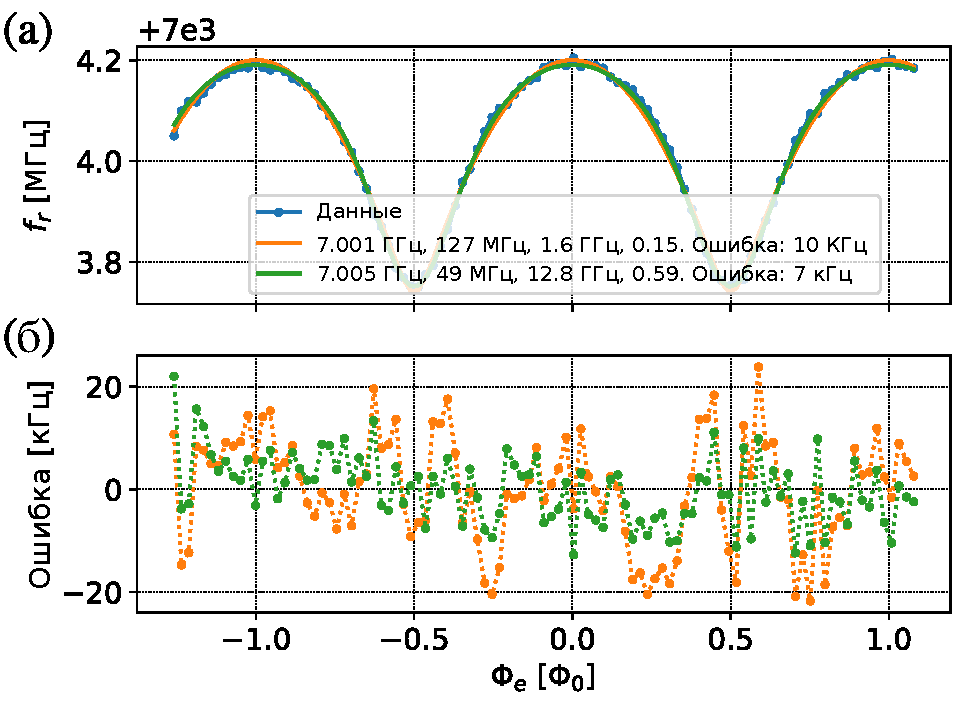
\includegraphics[width=0.7\linewidth]{Pictures/alternative_fits}
		\caption{\textbf{(а)} Две возможные аппроксимации (оранжевым и зеленым) одних и тех же данных (синим) моделями с различными параметрами $f_c,\ g,\ f_{ge}^\text{max},\ d$, указанными в легенде вместе со значением среднеквадратичной функции потерь на одну точку. \textbf{(б)} Разница между данными и двумя обозначенными моделями, где оранжевым показан случай максимальной частоты кубита ниже частоты резонатором, а зеленым -- минимальной частоты выше частоты резонатора.}
		\label{fig:alternativefits}
	\end{figure}
	
	В текущей программной реализации алгоритма есть и недостатки. В частности, шаг с полным перебором не выполняется параллельно, а в дальнейшем может быть заменен неким более изощренным глобальным методом оптимизации, как, например, имитацией отжига или \foreignlanguage{english}{basin-hopping} (см., например, \cite{wales1997global}), или осуществляться на адаптивной неравномерной сетке. Алгоритм в целом может испытывать проблемы при большой зашумленности данных в случае большой отстройки кубита и резонатора. Тогда два совершенно разных набора параметров дадут приблизительно одинаковое значение для функции потерь. Иллюстрацией этого утверждения является \autoref{fig:alternativefits}, на котором показаны результаты аппроксимации, полученные при запуске алгоритма на двух различных (не пересекающихся по диапазонам $f_{ge}^\text{max}$) сетках. Как видно, совпадение между данными и двумя моделями одинаково хорошее для двух случаев, несмотря на качественно различный смысл оптимумов. Это означает, что невозможно быть уверенным в истинности какого-то одного из них без какой-то дополнительной информации об образце. Для решения этой проблемы можно передавать алгоритму набор подсказок, например, что кубит следует искать ниже резонатора по частоте; такой подход эквивалентен наложения некоторого априорного распределения на параметры системы, поэтому можно сказать, что в дальнейшем можно заменить ММП на метод апостериорного максимума. В же противном случае потребуется проводить две последовательные ДТС для установления истинного положения дел, что, естественно, увеличит время измерений.
		
	\section{Компьютерное распознавание результатов двухтоновой спектроскопии}
	
	В предыдущем разделе был описан алгоритм распознавания результатов однотоновой спектроскопии. Теперь обратимся к рассмотрению следующего экспериментального шага -- двухтоновой спектроскопии. На \autoref{fig:detectiontts}~(а) изображен общий подход к задаче: из анализа данных ОТС можно получить приблизительную зависимость частоты кубита от тока $I$ или другого контролирующего параметра (мы будем называть её $f_{ge}^{(0)}(I)$). На основе этой приблизительной зависимости выбирается область сканирования для ДТС: это может быть окрестность верхней или нижней оптимальной точки, или какое-либо другое положение. После выполнения измерения данные передаются алгоритму распознавания, который, разумеется, должен принимать на вход также и $f_{ge}^{(0)}(I)$, так как это обеспечит максимальную его информированность об условиях эксперимента и дает возможность сравнительно просто решить поставленную задачу. Результатом работы алгоритма должны быть параметры кубита, описывающие форму аналитически выражений его спектральных линий. Опять же ограничиваясь пока что случаем трансмонов, такие линии отвечают одно-, двух-, трех- и т.д. фотонным переходам, которые мы будем обозначать соответствующей комбинацией латинских букв и знаком дроби. На \autoref{fig:detectiontts}~(б) показаны желаемые результаты распознавания на трех примерах реальных экспериментальных данных из нашей базы. Желательно, чтобы алгоритм мог работать в случае, когда сканирование происходит на диапазонах, близких к периоду по потоку, в случае малого отношения сигнал/шум и при наличии побочных линий, которые должны исключаться из рассмотрения. Возвращаемые кривые же должны максимально точно ложиться на данные, для чего логично снова положиться на метод максимального правдоподобия в форме наименьших квадратов. 
	
	
	\begin{figure}[t]
		\centering
		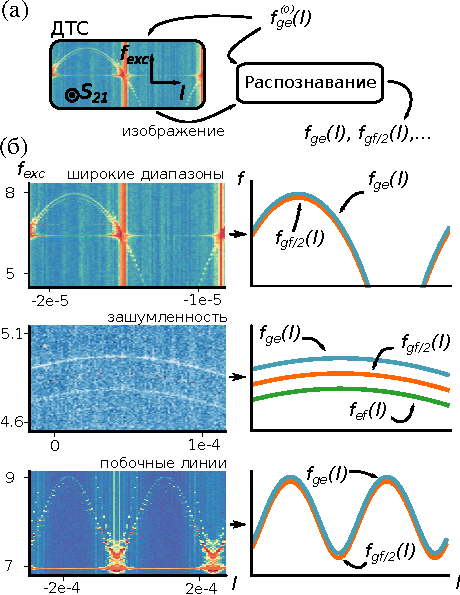
\includegraphics[width=0.6\linewidth]{Pictures/detection_tts}
		\caption{\textbf{(а)} Схематическое изображение принципа анализа результатов ДТС. Приблизительная зависимость частоты кубита $f_{ge}^{(0)}(I)$ от тока служит как для задания области сканирования, так и в качестве начального приближения для алгоритма распознавания. \textbf{(б)} Примеры желаемой работы алгоритма на различных типах данных.}
		\label{fig:detectiontts}
	\end{figure}
	
	Опишем здесь более детально процедуру получения двухтонового спектра \cite{wallraff2007} и те данные, которые она дает на выходе. Предположим, что на входе мы имеем данные ОТС, изображенные на \autoref{fig:extractpoints}~(а) и обработанные методами из прошлого раздела. Принцип двухтоновой спектроскопии заключается в ``прицеливании'' частоты $f_p$ в минимум резонансного провала для каждого значения тока так, чтобы можно было замечать изменение пропускания через него. Последнее наблюдается, например, при совпадении дополнительного развертываемого сигнала $f_{exc}$ с каким-то переходом кубита в силу их дисперсионного взаимодействия \cite{blais2004cavity, koch2007charge}. Получаемая картина в зависимости от частоты $f_{exc}$ и тока $I$ показана на \autoref{fig:extractpoints}~(б) (для лучшего понимания происходящего здесь стоит обратить внимание на то, что цветовая шкала на этом и предшествующем графиках одинакова). Как видим, большая часть данных окрашена в синие тона, что значит отсутствие какого-либо эффекта на резонансный пик; на этом фоне отчетлива видна основная линия трансмона, отвечающая переходу $ge$ и приходящая в оптимальную точку на частоте около 7.6 ГГц, и её сателлит -- двухфотонный переход $gf/2$. В других областях могут наблюдаться различные паразитные линии, например, самой яркой из таких является горизонтальная линия самого резонатора, расположенная около 6.5 ГГц. Также чуть выше наблюдается менее яркая горизонтальная линия от другого резонатора на том же чипе. Широкая вертикальная линия наблюдается, когда линия резонатора пропадает из области сканирования и становится трудно различимой, попадая в область квазипересечения. Научить измерительную программу автоматически не сканировать в этой области достаточно проблематично; напротив, как мы увидим, исключать эти области при последующей обработке данных не представляет трудностей.
	
	
	\begin{figure}[t]
		\centering
		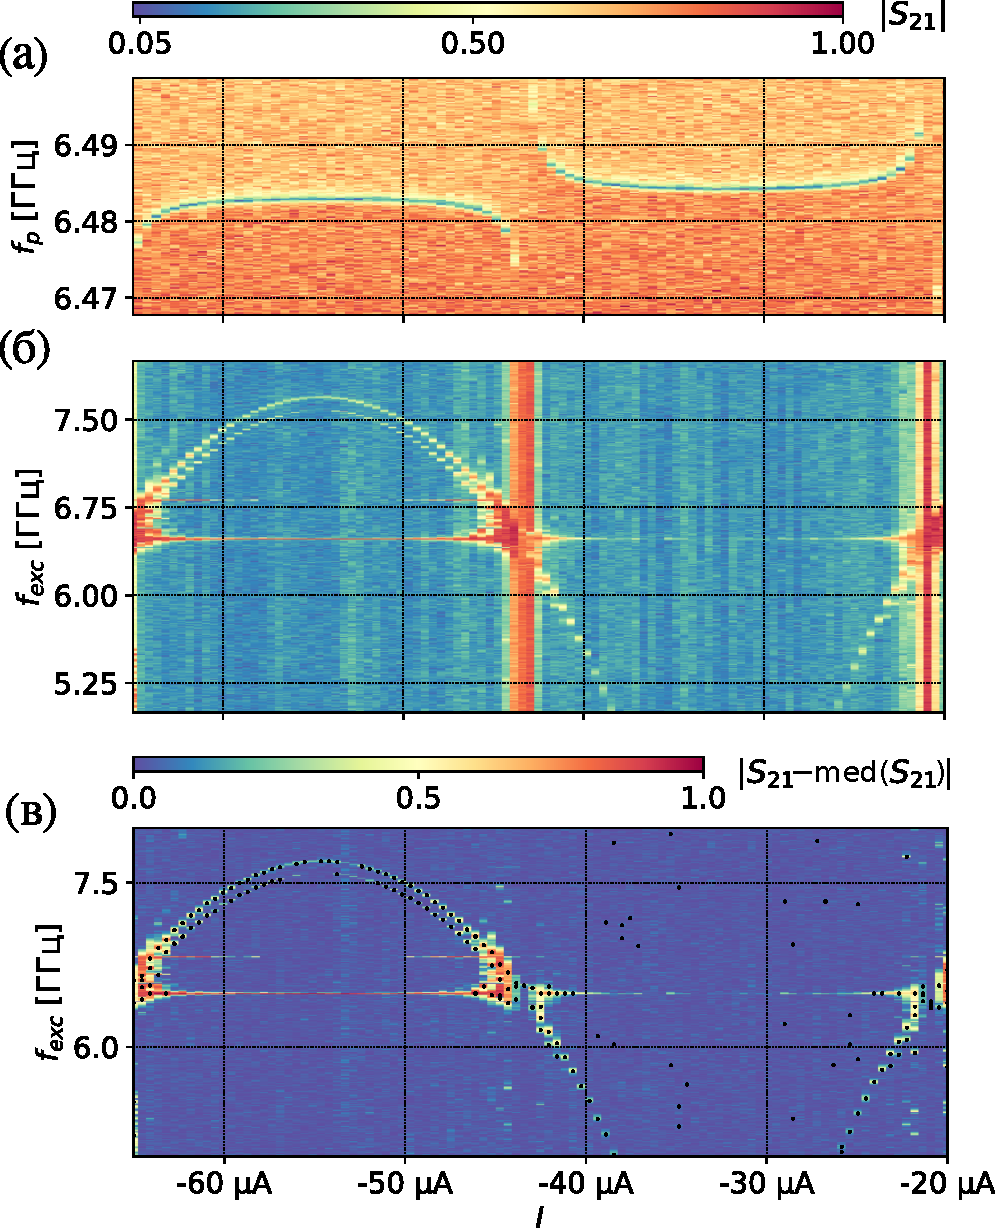
\includegraphics[width=0.6\linewidth]{Pictures/extract_points}
		\caption{\textbf{(а)} Данные однотоновой спектроскопии около частоты резонатора -- наблюдаются квазипересечения. \textbf{(б)} Данные двухтоновой спектроскопии. Кроме однофотонной и двухфотонной линий трансмона наблюдаются две горизонтальные линии от резонаторов и вертикальные линии, вызванные квазипересечениями. Цветовая шкала для (а) и (б) общая. \textbf{(в)} Данные с вычетом медианного значения по частоте для каждого тока. Черные кресты показывают локальные экстремумы, значение данных в которых превышает пороговое.}
		\label{fig:extractpoints}
	\end{figure}
	
	Как видно, структура данных ДТС не позволяет использовать готовые методы для аппроксимации кривых. Главной проблемой является наличие нескольких пиков для каждого значения тока, между которыми программе придется так или иначе делать выбор. К сожалению, без видения полной картины спектра (оперируя локальными данными только одного вертикального столбца данных) сложно установить соответствие между пиками и переходами. Таким образом, алгоритм должен получать на вход максимально упрощенный набор данных, исключающий, насколько возможно,  паразитные линии и шумы, в то же время сохраняя все осмысленные линии. В качестве альтернативного подхода можно было бы реализовать другое измерение -- например, проведя ОТС, установить кубит в оптимальную точку и произвести точный одномерный скан по частоте в зависимости от мощности излучения. Подобные картины можно видеть в предыдущих работах автора \cite{fedorov2017}, см. Рис. 1.24, 3.9, 3.24. Далее бы выполнялась аппроксимация каждого среза по мощности набором лоренцевых пиков, по их ширине выяснялось бы, к процессу какого порядка относится каждый из найденных в срезе пиков. Однако автору неизвестно, какие проблемы могли бы возникнуть в таком подходе; более того, задача обработки изображения целиком и поиска параметров нескольких линий, скрытых там, представляется намного более интересной в научном плане.
	

	\subsection{Предварительная обработка данных}
	
	На \autoref{fig:extractpoints}~(в) показаны предварительно обработанные данные из \autoref{fig:extractpoints} (б). Основными идеями при обработке являлись:
	\begin{itemize}
		\item сведение комплексных данных $S_{21}$ к действительным числам
		\item устранение вертикальных особенностей фона
		\item сведение данных к массиву пар координат 
		\item устранение узких горизонтальных линий
	\end{itemize}

	Первые два пункта решаются одновременно следующим образом. Рассчитаем для каждого значения тока комплексное медианное значение $\text{med}(S_{21})$. Затем построим величину $Z = |S_{21} - \text{med}(S_{21})|$, где формула понимается в том смысле, что из каждой колонки данных вычитается ей соответствующая константа. На \autoref{fig:extractpoints}~(в) эта величина построена цветом. Такое построение не только исключает практически все вертикальные полосы, сохраняя осмысленные данные без изменений и выравнивая их фон, но и позволяет одинаково хорошо замечать отличия как по амплитуде, так и по фазе $S_{21}$.
	
	Далее алгоритм должен определить, какие точки данных интересны, а какие можно исключить. Для этого логично применить пороговый метод, который оставит для анализа лишь одномерный массив координат. Автором рассматривались разные подходы, в частности, метод Оцу \cite{otsu1979}, однако было выяснено, что лучше всего для данной задачи работает более узкоспециализированный метод, основанный на предварительном выявлении локальных максимумов при помощи прямого перебора и сравнения точек, реализованный функцией \foreignlanguage{english}{scipy.argrelextrema}. Так как из-за шума экстремумов находится в каждом столбце гораздо больше, чем там есть настоящих спектральных линий, мы, во-первых, ограничиваем максимальное число пиков тремя самыми высокими, а во-вторых, исключаем все пики, высота которых меньше, чем пороговое значение. Эмпирически было установлено, что можно установить его равным медианному значению абсолютной величины дискретного дифференциала данных по направлению оси $f_{exc}$
	\begin{equation}
		\sigma = \text{med}(|Z_{i,j+1} - Z_{i, j}|),
	\end{equation}
	где $i$ и $j$ нумеруют токи и частоты, соответственно, а усреднение проводится по всему двумерному массиву. Эта величина характеризует уровень шумов при переходе от точки к точке и должна вычисляться для каждого эксперимента отдельно в силу их непредсказуемости. Здесь особенно важно использование медианного значения, которое позволяет существенно уменьшить влияние пиков сигнала на оценку шума.
	
	После указанных шагов алгоритм получает набор точек, соответствующих наиболее ярким пикам. На этом этапе уже можно исключить горизонтальные линии: если в массиве обнаруживается определенное количество точек, у которых значение $f_{exc}$ совпадает в пределах разрешения сетки, все они отсеиваются, как принадлежащие одной горизонтальной линии, на чем и заканчивается предварительная обработка. На \autoref{fig:extractpoints} извлеченные точки показаны крестами. Как видно, горизонтальные линии исключаются из массива точек, основные линии хорошо представлены, а шумовые точки практически не учитываются. Исключение составляют области, где спектральная линия кубита не видна совсем: там шумовые пики все равно определяются. Повышение порога в таком случае не подходит, так как тогда будут потеряны слабо видимые точки перехода $gf/2$.
	
	\subsection{Описание алгоритма}
	
	
	\begin{figure}
		\centering
		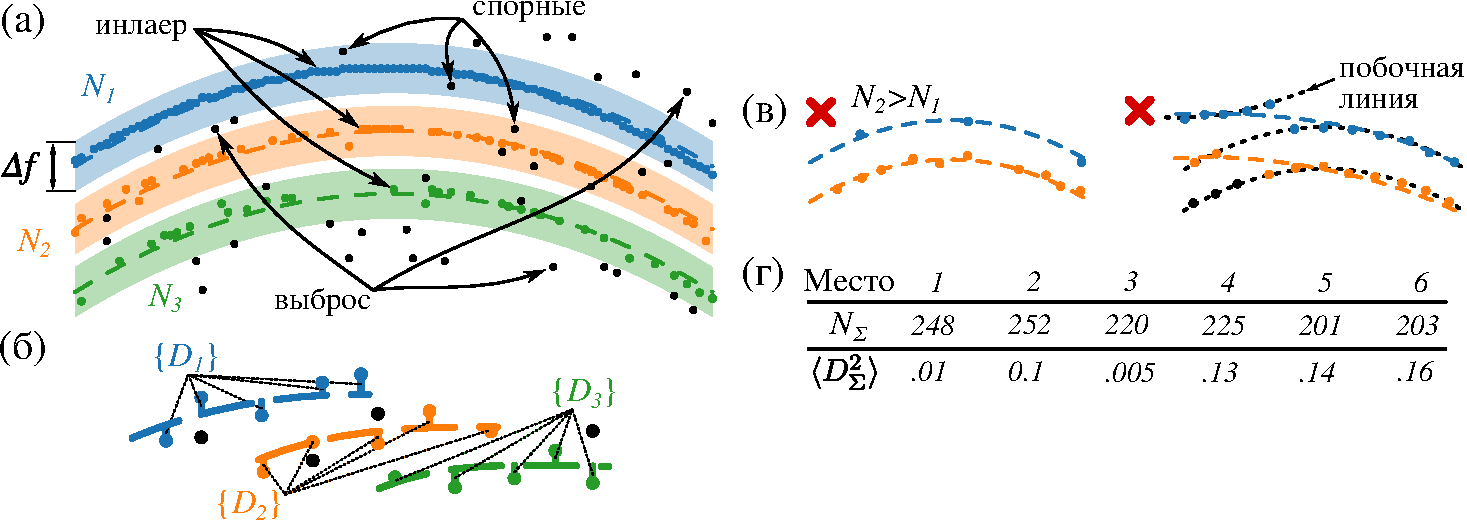
\includegraphics[width=\linewidth]{Pictures/hough_illustration}
		\caption{\textbf{(а)} Вокруг каждой модельной кривой берется симметричный интервал частот шириной $\Delta f$ (выделенные цветом области). Для каждого тока точки вне интервала называются выбросами; из остальных выбирается единственная (ближайшая к модели) точка из интервала -- инлаер, оставшиеся -- спорные. \textbf{(б)} По инлаерам для каждой модели вычисляются среднеквадратичные расстояния $\{D_{1-3}\}$. \textbf{(в)} Дополнительные условия. На основной линии кубита не должно быть меньше точек, чем на какой-либо из побочных; максимизация числа точек не должна происходить за счет ухудшения качества аппроксиммации. \textbf{(г)} Иллюстрация сортировки найденных перебором решений. В первую очередь учитывается число точек (см. текст), затем среднеквадратичное отклонение данных от модели.}
		\label{fig:houghillustration}
	\end{figure}


	Как видно, даже после обработки данные содержат большое количество лишних точек, которые надо исключить особым образом; более того, для более эффективной идентификации кубита и отличения его от побочных линий надо использовать максимум информации о структуре спектра, ему присущей. Для трансмона это подразумевает одновременную аппроксимацию сразу нескольких линий, включающих как основной, так и многофотонные переходы. Для решения этой проблемы автором предлагается гибридный алгоритм, объединяющий в себе черты преобразования Хафа \cite{hough1962} и алгоритма случайной подвыбрки RANSAC \cite{fischler1981}. Здесь также стоит отметить, что для многомодельной оптимизации на данных, весьма напоминающих по своей структуре наши, относительно недавно был разработан, например, специальный метод под названием PEARL \cite{isack2012energy} и другие (CORAL \cite{amayo2018geometric}, Progressive-X \cite{barath2019progressive}), но пока что в свободном доступе готовую к использованию реализацию их найти нельзя, а модели, на которых они тестировались, были линейными. Не исключая возможности того, что указанные алгоритмы окажутся не менее действенными, мы развиваем свой подход и отлаживаем его для конкретной проблемы.
	
	Основная идея алгоритма иллюстрируется на \autoref{fig:houghillustration} (а). Для того, чтобы можно было исключать точки, заведомо не попадающие ни на какую из кривых, вокруг каждой модельной кривой выбирается область частот шириной $\Delta f$, и все точки, которые находятся за её пределами, к этой кривой не приписываются (точки, которые не принадлежат ни одной из кривых, будут называться выбросами, как в RANSAC). Далее, из тех точек, которые попадают в область одной из кривых, выбираются ближайшие к ней, их будем называть инлаерами (от англ. \foreignlanguage{english}{\textit{inliers}}), а остальные -- спорными точками.  Далее для $i$-той кривой вычисляются наборы отклонений кривых от своих инлаеров $\{D_i\}$, нормированная сумма квадратов которых будет оценкой качества приближения точек моделью, $\langle D^2_\Sigma\rangle = 1/N_\Sigma \sum_i \sum \{D_i^2\}$, где $N_\Sigma = \sum N_i$ -- суммарное число инлаеров. В преобразовании Хафа параметры модели, обеспечивающие максимальное $N_\Sigma$, считаются истинными. Однако, как показано на \autoref{fig:houghillustration} (в), в некоторых случаях такое решение окажется неверным. Например, алгоритм может выбрать параметры так, что основная линия попадет на побочную линию модели, в то время как основная линия модели соберет случайные точки над ней. Другой случай -- когда побочная линия забирает приоритет на себя, давая небольшое преимущество по количеству точек. Для решения этой проблемы используется, во-первых, условие необходимого преобладания количества точек на основной кривой, а во-вторых, учет среднеквадратических отклонений, как в RANSAC. Осмысленно сортировать результаты по среднеквадратическим отклонениям возможно только при условии, что числа инлаеров у них одинаковы. Так как в реальности этого быть не может, мы дополнительно устанавливаем шаг $N_b$ по количеству точек в 10\% от общего числа значений тока $M$. Внутри каждой группы точек затем происходит сортировка по $\langle D^2_\Sigma\rangle$. На \autoref{fig:houghillustration} (г) в качестве примера показана конечная таблица, в которой на первом месте оказывается модель с 248 точками (при максимуме в 252, но с гораздо худшим $\langle D^2_\Sigma\rangle$). 
	Составление таблицы происходит в процессе полного перебора параметров модели по сетке на основе первого приближения, которое получается из ОТС.
	
	После составления сетки и выбора лучшего кандидата запускается алгоритм локальной оптимизации. Для него уже нельзя использовать двойную сортировку, как в таблице на \autoref{fig:houghillustration} (г), но необходимо иметь функцию потерь, которая бы сохраняла смысл процедуры. Мы предлагаем использовать следующую функцию, использующее группированное число точек $[N_\Sigma/N_b]\cdot N_b$ (скобки означают округление до целого числа):
	\begin{equation}
	\mathcal{L}_{N\text{-}M} = \frac{1}{[N_\Sigma/N_b]\cdot N_b} + \langle D_\Sigma^2 \rangle.\label{eq:loss_tts}
	\end{equation}
	В правой части второе слагаемое имеет единицы частоты, поэтому в реализации алгоритма надо брать только численное значение в ГГц. Так как обычно расстояния между кривой и точкой не превышают $\Delta f < 100$ МГц, второе слагаемое не принимает больших значений и обеспечивает сортировку лишь внутри группы (характерныя значенiя $N_\Sigma < 500$, $M < 200$).
	
	
	\begin{table}
		\centering
			\small
			\begin{tabular}{c*4c}\toprule 
				\multicolumn{2}{c}{Оптимизация} & $I_{sws}$ & $f_{ge}^\text{max}$ &  	$d$\\
				\midrule
				\multirow{2}{*}{\makecell{Перебор 1\\ $\Delta f$=100 МГц}} & диап. & $I_{ss}^{(0)}\pm .05\, \Pi^{(0)}$ & $f_{ge}^{\text{max}, (0)}\pm 1.5$ ГГц & 0.1 - 0.9  \\
				& точек & 10& 50& 8\\\hline
				\multirow{2}{*}{\makecell{Перебор 2\\ $\Delta f$=50 МГц}} & диап. & $I_{ss}^{(1)}\pm .02\, \Pi^{(0)}$ & $f_{ge}^{\text{max}, (1)}\pm 100$ МГц & $d^{(1)}\pm 0.1$ \\
				& точек & 10 & 20 & 10\\
				\bottomrule
			\end{tabular}
		\caption{Параметры сетки для полного перебора при предварительной грубой и грубой оптимизации по одной линии.}
		\label{tab:grid_tts}
	\end{table}

	На практике мы разбиваем оптимизацию полным перебором на три шага. Первые два шага оптимизируют лишь одну модельную кривую. В таблице \autoref{tab:grid_tts} указаны соответствующие параметры сетки, построенной для начальных значений $\Pi^{(0)},\ I_{ss}^{(0)},\ f_{ge}^{\text{max}, (0)},\ d^{(0)}$, полученных из ОТС. Как видно, на первом шаге используется увеличенный интервал частот, чтобы найти примерное расположение кривой при широком диапазоне перебора параметров $f_{ge}^\text{max}$ и $d$. В то же время, период $\Pi$ и положение оптимальной точки $I_{ss}$ оставляются практически без изменений по сравнению с однотоновой оптимизацией (последнее может несколько смещаться, если эксперименты проводятся с большой задержкой по времени, однако при немедленном выполнении ДТС после ОТС перебор по этому параметру не требуется). Оптимальные параметры, полученные после этого шага, обозначим как $f_{ge}^{\text{max},(1)}...$ и т.д. На втором шаге окно частот сужается и параметры найденной линии определяются уже с большей точностью и записываются как $f_{ge}^{\text{max}, (2)}...$ и т.д. На этом этапе алгоритм может найти любую из кривых, соответствующих однофотонному или одному из многофотонных переходов, так как неизвестно, на которой из кривых будет обнаружено большинство точек; без одновременной аппроксимации сразу несколькими линиями надежно бороться с этим эффектом нельзя, а, значит, нельзя полагаться на значение $f_{ge}^{\text{max}, (3)}$. В то же время, значение $d$ при фиксированном $\Pi$ здесь определяется достаточно хорошо. Далее, на найденных инлаерах запускается алгоритм Нелдера-Мида с функцией потерь \eqref{eq:loss_tts}, который устанавливает параметры найденной кривой с большой точностью.
		
	Наконец, переходим к многомодельной оптимизации в полном соответствии с \autoref{fig:houghillustration}. Так как для трансмона главная и побочная спектральные линии отличаются друг от друга лишь параллельным переносом вдоль вертикальной оси \cite{fedorov2017} на величину, равную целому числу полуангармонизмов трансмона $\alpha/2$, алгоритму достаточно перебирать значения его и $f_{ge}^\text{max}$. Параметры сетки перебора указаны в \autoref{tab:tts_grid_multi}; так как остальные параметры хорошо определены, для успешной работы обычно достаточно всего 100 точек. Также, раз побочные линии трансмона располагаются под основной, для $f_{ge}^\text{max}$ необходимо строить сетку только выше значения $f_{ge}^{\text{max}, (3)}$, обеспечивая движение гребенки линий только вверх. Верхний предел обусловлен величиной ангармонизма, который обычно не превышает 300 МГц. После выполнения этого шага в большинстве случаев модельные кривые встает точно на спектральные линии, и снова запускается симплекс-алгоритм для окончательной полировки решения.
		
	\begin{table}
		\centering
		\small
		\begin{tabular}{ccc} \toprule
			Параметр & Диапазон & Точек \\
			\midrule
			$f_{ge}^\text{max}$ & $f_{ge}^{\text{max}, (3)}  \substack{+0.4\ \text{ГГц} \\ -0.0\ \text{ГГц}}$  & 10 \\
			$\alpha$ & 0.2-0.3 ГГц & 10 \\
			\bottomrule
		\end{tabular} 
		\caption{Параметры сетки при многомодельной оптимизации; $\Delta f = 50$ МГц для каждой модели.}
		\label{tab:tts_grid_multi}
	\end{table}

\subsection{Результаты}


\begin{figure}
	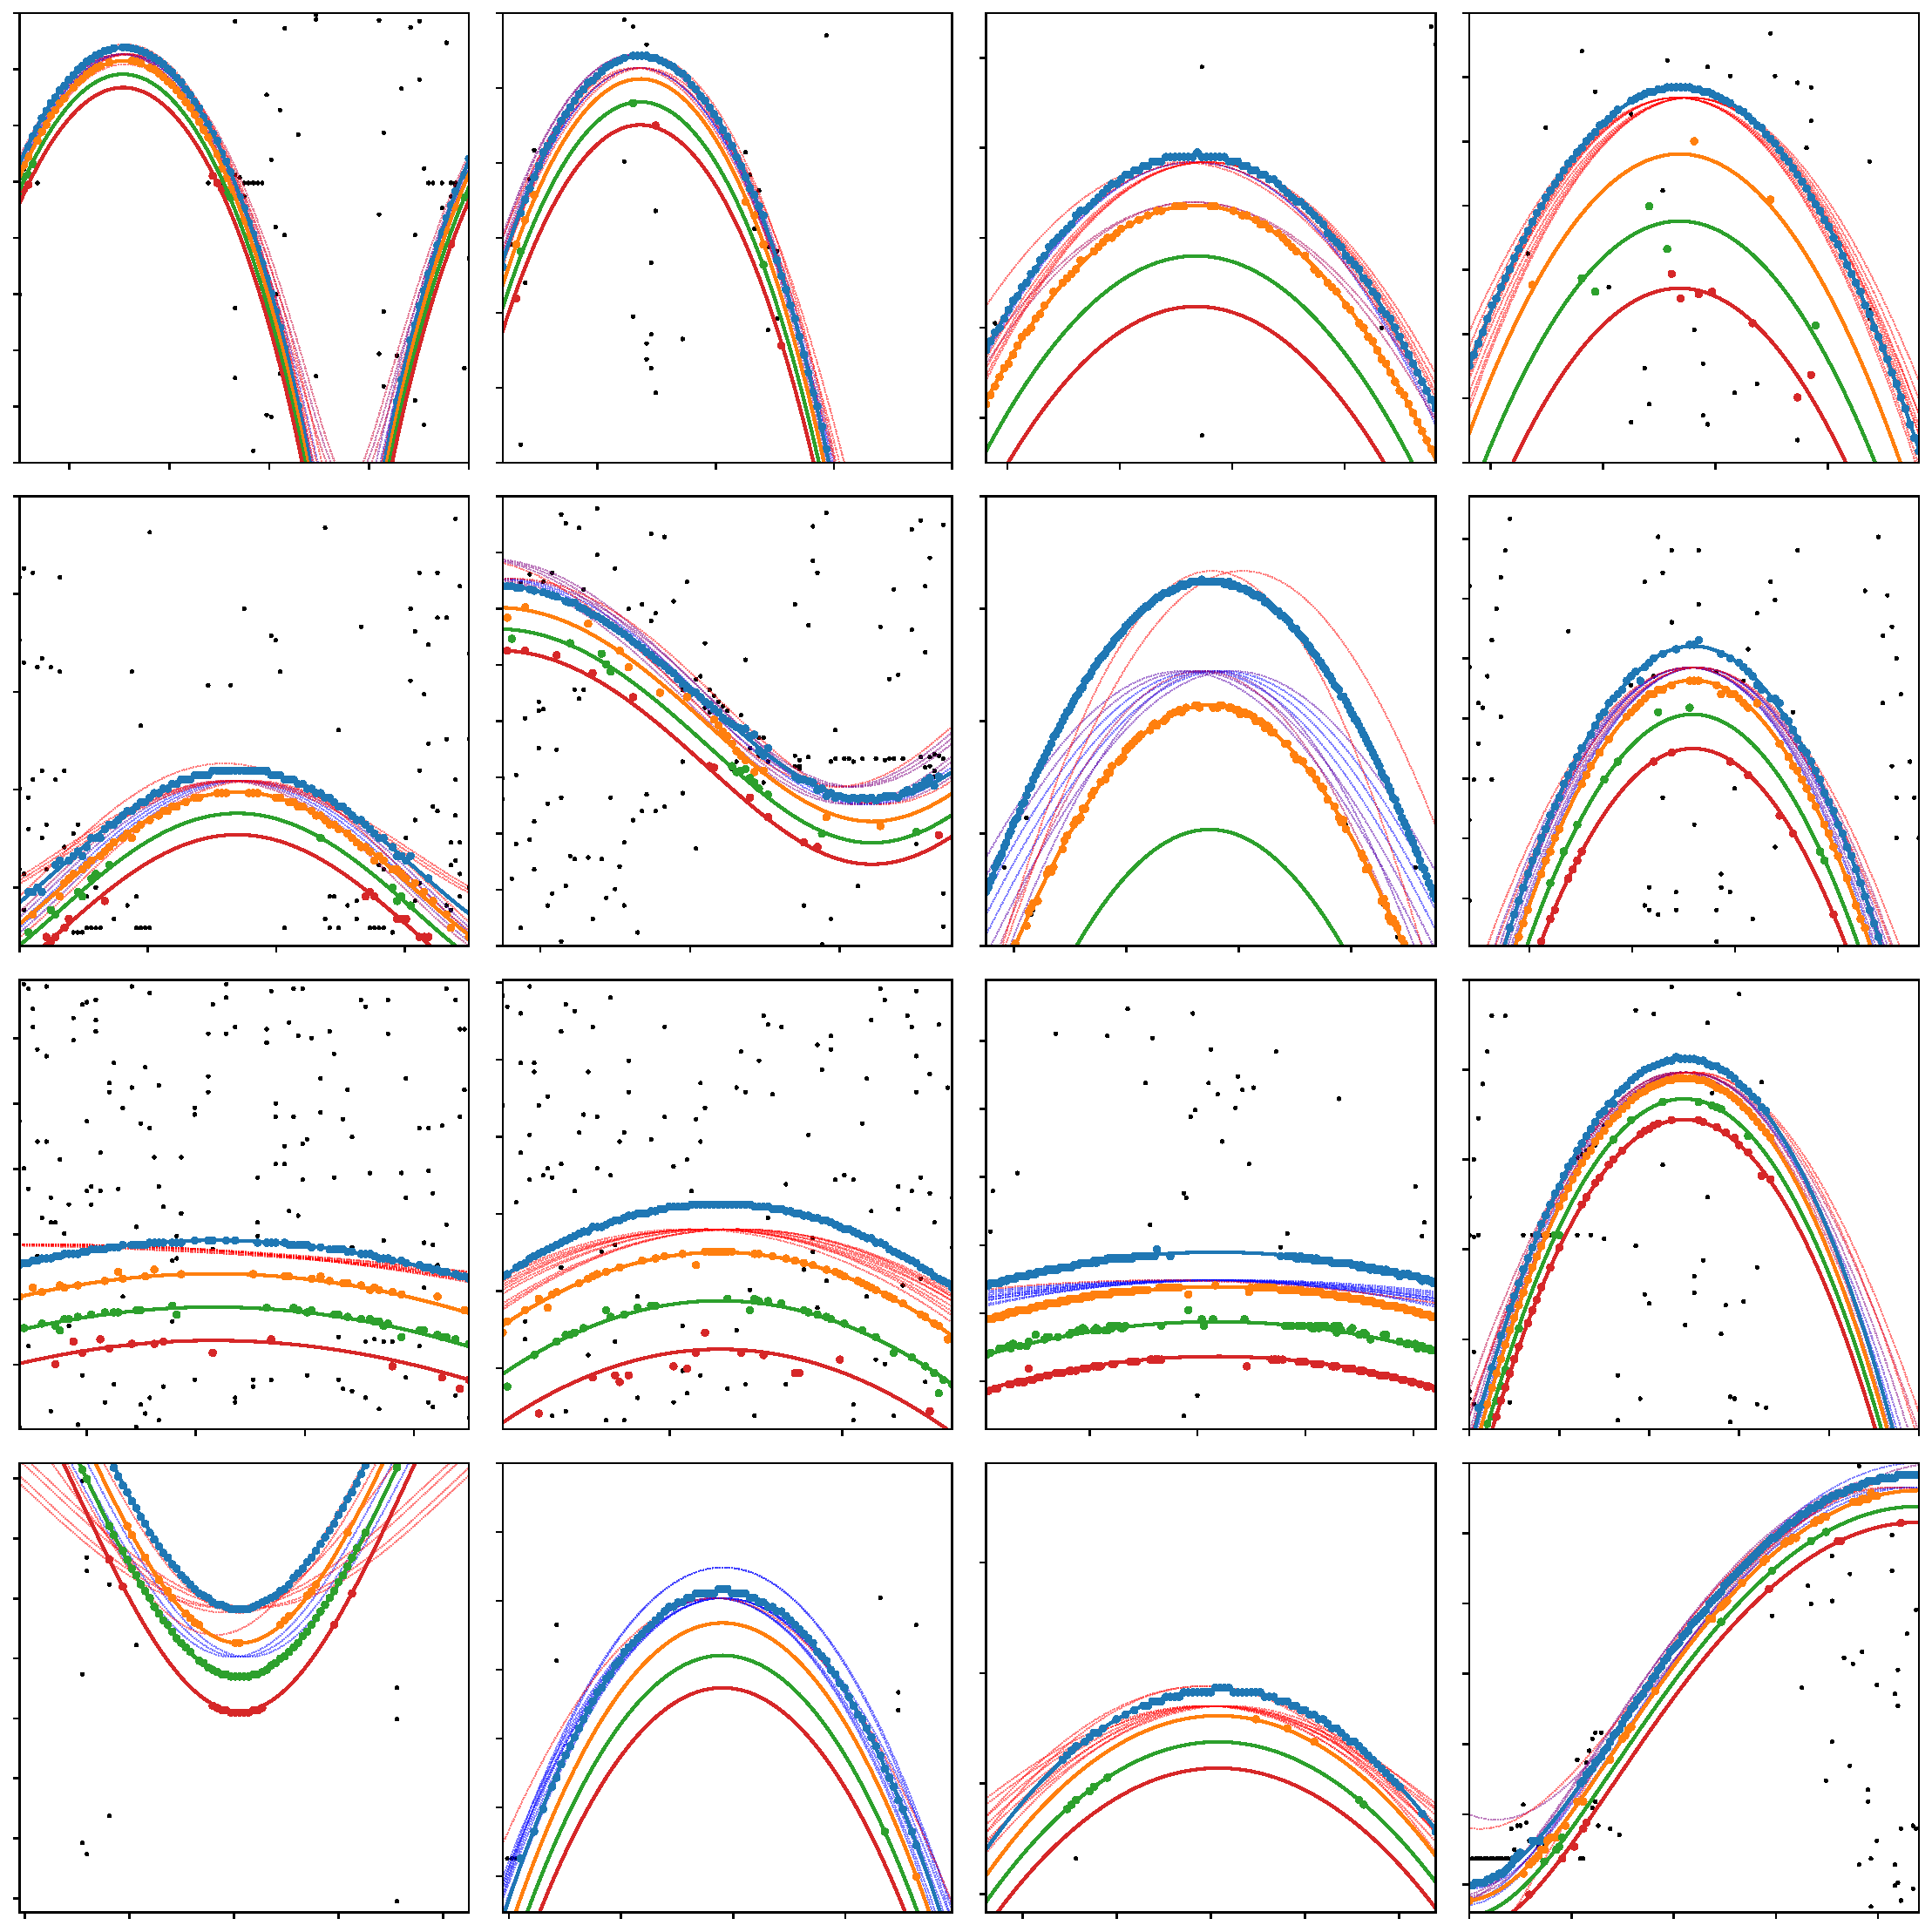
\includegraphics[width=1\linewidth]{Pictures/two_tone_fits}
	\caption{Результаты работы алгоритма на некоторых экспериментальных спектрах. Метапараметры фиксированы, выполнение проводилось в простом цикле по данным и начальным приближениям, полученным при распознавании соответствующих результатов ОТС. Черными точками показаны выбросы, присутствовавшие после предварительной обработки; цветами обозначены аппроксимированные модельные линии и их инлаеры (см. \autoref{fig:houghillustration}~(a)). Тонким пунктиром показаны десять лучших кандидатов, найденных в первом шаге грубой оптимизации (см. текст).}
	\label{fig:twotonefits}
\end{figure}


Реализация алгоритма на языке Python хранится в открытом доступе на GitHub, файл \foreignlanguage{english}{\textit{fulaut/SpectrumOracle.py}} \cite{fedorov2021github}. На \autoref{fig:twotonefits} представлены результаты тестового прогона алгоритма на реальных экспериментальных данных из нашей базы. Как видно, во всех 16 случаях программа превосходно справляется с задачей распознавания. Основным условием для корректной работы является достоверно заданный в начальном приближении период по потоку, в то время как в определении остальных параметров могут быть допущены относительно большие погрешности. Устойчивость алгоритма в этом контексте обеспечивается наличием первого шага грубой оптимизации. Отметим, что в текущей реализации основным критерием успеха является точность предварительной аппроксимации данных одной кривой на втором шаге грубой оптимизации. Для наглядности на \autoref{fig:twotonefits} показана также лидирующая десятка кривых-кандидатов, найденных в процессе первого шага грубого поиска с окном в 100 МГц (синим показаны самые лучшие из них, красным -- худшие, либо в одинаковом случае). Видно, что алгоритм здесь, как и было задумано, определяет лишь примерное расположение кривых, однако этого оказывается достаточно для успешной отработки следующего шага.

Выполнение алгоритма на Intel i5-3337U @ 2.5 ГГц занимает около 7.5 секунд. Основное время (3.2 с) приходится на первый шаг грубой оптимизации, затем следует многомодельная аппроксимация (2.5 с) и, наконец, второй шаг грубой оптимизации (1.8 с). Этапы полного перебора в целом работают значительно дольше (примерно в 4 раза), чем этапы локальной оптимизации алгоритмом Нелдера-Мида.

В процессе подготовки данного раздела автор проводил дополнительные эксперименты по предварительной обработке данных и пришел к выводу, что возможно усовершенствовать алгоритм, избавившись от полного перебора в первом шаге грубой оптимизации. Для этого предлагается использовать алгоритм, в большей степени похожий на RANSAC, чем на преобразование Хафа, однако с важной модификацией. Итерация алгоритма выглядит следующим образом:
\begin{itemize}
	\item Осуществляем случайную выборку без возврата 50\% точек из массива данных с использованием некоторого постоянно обновляющегося распределения вероятности (на первой итерации оно равномерное)
	\item При помощи функции \foreignlanguage{english}{\textit{curve_fit}} осуществляем аппроксимацию выбранного массива точек
	\item Рассчитываем расстояния от полученной модели уже до всех точек массива данных
	\item Выбрасываем несколько точек с наибольшими ошибками, обновляя массив данных
	\item Задаем распределение вероятности по оставшимся точкам обратно пропорционально величине их расстояний до модели (искусственно задаем нижний предел расстояния в 1 МГц, чтобы исключить выбросы в распределении при случайных совпадениях точек и модели)
\end{itemize}

На текущий момент реализация этого алгоритма еще не доведена до совершенства, поэтому дальнейшее обсуждение мы оставляем за рамками данной диссертации.

\subsection{Заключение}

Автором был предложен и реализован алгоритм распознавания данных ДТС для сверхпроводниковых кубитов типа трансмон в условиях неизбежного присутствия большого количества шумовых данных и сложной структуры спектра, состоящего из нескольких линий одинаковой формы. Алгоритм прост, не является стохастическим и выполняется за фиксированное время при фиксации метапараметров поиска. Точность нахождения параметров трансмона такая же, как была бы при отсутствии шума; более того, за счет того, что осуществляется многомодельная аппроксимация, метод позволяет точно идентифицировать и величину ангармонизма трансмонов. Идея алгоритма позволяет его обобщение и на другие типы кубитов, в частности, на потоковые, где спектральная линия чаще всего одна и представляет собой гиперболическую кривую. Многофотонные переходы в таких кубитах имеют существенно отличную и сложную форму, поэтому, вероятно, потребуются более существенные модификации в части многомодельной оптимизации.

\section{Выводы по Главе 2}

Автором были подробно описаны основные экспериментальные установки и методы, использующиеся при работе со сверхпроводниковыми квантовыми устройствами. Были описаны проблемы, возникающие из-за необходимости автоматизировать измерения, подходы к их решению программными методами, общее описание процесса экспериментов. Наконец, автором были описаны два алгоритма для решения проблемы интерпретации данных спектроскопии, необходимой для калибровки физических параметров образца и перехода к выполнению квантовых алгоритмов или других операций, требующих определения характеристик образца. Предложенные программы значительно облегчают работу экспериментатора и активно используются как самим автором, так и его коллегами в лабораториях МФТИ, МИСиС и др.

\chapter{Гибридизация излучения с двухатомной искусственной молекулой}

\section{Введение}

За последние 20 лет многочисленные исследования убедительно показали, что сверхпроводниковые искусственные атомы (СИА) действительно подчиняются как фундаментальным законам квантовой механики, так и их сложным и разнообразным следствиям \cite{you2011atomic, gu2017microwave}. Благодаря тому, что гамильтонианы этих систем можно заранее проектировать, они оказались особенно гибким инструментом для исследований в области квантовой оптики; кроме того, высокая точность управления их параметрами in situ позволяет обнаруживать новые физические эффекты, недоступные при наблюдении естественных систем.

Одним из наиболее значительных результатов в этом контексте является достижение сильной связи с излучением в КЭД цепей \cite{wallraff2004strong, chiorescu2004coherent}, когда частота вакуумных осцилляций Раби превышает скорости релаксации и декогеренции.  На текущий момент на сверхпроводниковых схемах реализация сильной связи с излучением является самой совершенной в терминах когерентности \cite{forn2019ultrastrong}, подтверждая тем самым уникальность данной платформы для экспериментов по квантовой оптике. Однако, в отличие от естественных атомов и молекул, для реализации сильной связи СИА со светом не требуется использовать резонаторы с удерживаемым внутри них излучением (это дает возможность увеличить связь за счет эффективно многократного взаимодействия ЭМ волны с системой \cite{blais2004cavity}). Искусственные атомы могут связываться очень сильно и со свободно распространяющимся светом \cite{astafiev2010resonance}, если последний помещен в одномерный волновод. В таких архитектурах частота Раби может достигать 50\% от частоты резонансного перехода \cite{deng2015observation}, что оказывается уже скорее в области сверхсильной связи (\foreignlanguage{english}{\textit{ultrastrong coupling}}). Чтобы правильно описывать поведение атома в таком режиме, используется формализм т.н. одетых состояний: излучение должно быть явным образом включено в гамильтониан и будет модифицировать собственные состояния, гибридизуясь с ними. 

К настоящему времени в литературе описано множество экспериментов по квантовой оптике на чипе (\foreignlanguage{english}{\textit{on-chip quantum optics}}), обнаруживающими эффекты подобной гибридизации СИА с излучением большой интенсивности \cite{baur2009measurement, sillanpaa2009autler, astafiev2010resonance, novikov2013autler, suri2013observation, koshino2013observation, braumuller2015multiphoton, peng2018vacuum, gasparinetti2019two}. Во всех указанных работах одетые состояния проявляются через триплеты Моллоу или различного характера расщепления из-за эффекта Отлера-Таунса (ЭОТ). Однако, несмотря на недавние успехи в создании больших массивов взаимодействующих СИА \cite{Song574, ye2019propagation, arute2019quantum}, поведение таких составных систем при облучении полями большой интенсивности пока еще не исследовалось. Следует отметить, что исследовались одетые состояния многокубитных систем в резонаторах \cite{fink2009dressed, macha2014implementation, shulga2017observation, yang2018probing}, однако взаимодействие со свободным полем представляет не меньший интерес, так как его частоту можно легко приводить в резонанс с любым из переходов в системе. Более того, величину связи для свободного излучения можно эффективно регулировать, изменяя его интенсивность, в то время при гибридизации с резонаторами она чаще всего жестко задана параметрами образца.

В данной главе представлены результаты исследований пары сильно связанных друг с другом искусственных атомов: сверхпроводящей искусственной молекулы (СИМ) \cite{kou2017fluxonium}. В нашем случае она состояла из двух трансмонов типа ``иксмон'' \cite{koch2007charge, barends2013coherent}, взаимодействие между которыми осуществлялось опосредованно через виртуальный обмен фотонами в резонаторе \cite{majer2007coupling} и непосредственно через емкостную связь. Микроволновое излучение направлялось на систему через копланарный волновод, расположенный на чипе, а считывание состояние молекулы может быть осуществлено при помощи т.н. совмещенного дисперсионного считывания  (\foreignlanguage{english}{\textit{joint dispersive readout}}) \cite{filipp2009two, chow2010detecting}. Проводя спектроскопическое исследование СИМ с высоким разрешением по частоте, автором было обнаружено, что интенсивный микроволновый сигнал не только рождает в ней богатый по своему многообразию набор многофотонных переходов, но и значительно изменяет структуру энергетических уровней. Даже в простой двухатомной молекуле это приводит к появлению сложных эффектов, сродных ЭОТ, с участием одно- и многофотонных процессов, которые могут быть объяснены только в модели одетых состояний. Несмотря на то, что расщепления ЭОТ исследуются давно и широко представлены в литературе (в том числе, в естественных молекулах \cite{tamarat1995pump, ahmed2012autler}), были обнаружены качественно новые спектроскопические проявления эффекта в случае, если молекула облучается несимметрично. Подобные эффекты в литературе до сих пор не описывались, так как прошлые работы по ЭОТ изучали либо единичные атомы \cite{baur2009measurement, 
sillanpaa2009autler, astafiev2010resonance, 
novikov2013autler, 
koshino2013observation, 
braumuller2015multiphoton, peng2018vacuum, 
gasparinetti2019two}, либо описывали \cite{suri2013observation} только стандартные спектральные черты эффекта, хорошо известные из квантовой оптики 20 века. Если расширить круг поиска и рассмотреть в целом эксперименты по спектроскопии связанных трансмонов, то обнаруживается, что и здесь ничего подобного не наблюдали, так как либо использовались сигналы малой мощности, что позволяло различить только основные однофотонные линии \cite{majer2007coupling, filipp2011multimode}, либо для возбуждения переходов на верхние энергетические уровни подавался сигнал с двумя различными частотными компонентами \cite{dicarlo2009demonstration}, либо разрешение данных было недостаточным \cite{kounalakis2018tuneable}, либо использовались неперестраиваемые по частоте трансмоны \cite{poletto2012entanglement} (в дальнейшем станет понятно, почему каждая из этих проблем препятствует наблюдению эффекта). Эксперименты с натуральными молекулами также не фиксировали подобного поведения, что неудивительно, так как трудно исследовать изолированную молекулу, не говоря уже о том, чтобы индивидуально контролировать частоты переходов атомов, из которых она состоит, что физически невозможно.

Представленные в данной главе результаты представляют ценность для молекулярной физики и квантовой оптики, не ограничиваясь лишь джозефсоновскими сверхпроводниковыми системами. В сходных условиях они могут проявляться в любой двухатомной системе вне зависимости от её природы, что особенно важно в контексте текущих исследований в области модификации спектров молекул светом \cite{hertzog2019strong}. Отметим, что здесь также будет полезен и теоретический аппарат, разработанный автором для количественного описания явления. В сверхпроводниковых квантовых схемах исследованные эффекты важны и для квантовых вычислений: экспериментатор должен следить за мощностью сигналов и учитывать возможные сдвиги частот (например, мы покажем, что операция bSWAP \cite{poletto2012entanglement} прямо подвержена влиянию найденных эффектов). Наконец, спектроскопия на высокой мощности позволяет получит информацию о высших энергетических уровнях системы используя минимальный набор приборов; данный подход может облегчить масштабирование электроники для управления квантовыми процессорами, представляющее на данный момент серьезные трудности \cite{hornibrook2015cryogenic}.

\section{Описание экспериментального образца}


\begin{figure}
	\centering
	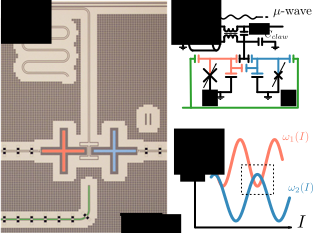
\includegraphics[width=0.7\linewidth]{Pictures/experiment_2}
	\caption{\textbf{(а)} Оптический микрограф устройства (в ложном цвете). Два трансмона (оранжевый, 1 и синий,2) связаны с  копланарным резонатором. Линии управления частотой подходят с боков, снизу подведена микроволновая антенна (зеленый). \textbf{(б)} Эквивалентная электрическая схема. Как перестраиваемые джозефсоновские переходы изображены СКВИДы трансмонов, управляемые магнитным полем. \textbf{(c)} Схематический рисунок частот кубитных переходов трансмонов $\omega_1 (I)$ и $\omega_2 (I)$ в зависимости от тока внешнего соленоида при правильном выравнивании локальными потоковыми линиями. Пунктиром обведена рабочая область эксперимента.}
	\label{fig:experiment2}
\end{figure}


Автором вместе со студентом магистратуры В. Юрса были разработаны технологические послойные чертежи для СИМ на основе пары перестраиваемых по частоте иксмонов с асимметричным СКВИДами \cite{hutchings2017tunable}. Они емкостно связаны с общим резонатором шунтирующего типа \cite{probst2015efficient} ($f_r = 7.34$ ГГц, $Q_e\approx$ 1900, $Q_l\approx$ 1100) длиной $\lambda/4$, использующимся для дисперсионного считывания состояния СИМ \cite{chow2010detecting}. На \autoref{fig:experiment2}~(а) представлена фотография устройства, полученная на оптическом микроскопе и показывающая физическое расположение элементов. Резонатор подсоединен к копланарному волноводу, через который осуществляется передача сигнала на считывание. Открытым концом он подсоединен к кубитам через специальный двойной встречно-штыревой конденсатор \cite{barends2013coherent}. Потоковые линии контроля частоты подходят с двух сторон, волновод для возбуждения переходов подает микроволновый сигнал снизу. Эквивалентная электрическая схема изображена на \autoref{fig:experiment2}~(б). Здесь считывающий резонатор емкостно и индуктивно связан с передающей линией, что является упрощением, подобным использованному в работе \cite{khalil2012}, хотя существует и более строгий подход \cite{besedin2018quality}. Как можно видеть, связь между трансмонами имеет двойственную природу: они связаны как через резонатор \cite{majer2007coupling, filipp2009two}, так и напрямую емкостным образом, причем оба этих механизма дают вклад в наблюдаемую в эксперименте силу связи (причем с противоположными знаками). Причину этого легко можно видеть на оптической фотографии образца -- острова трансмонов из-за своего большого размера могут электрически влиять друг на друга, имея ненулевую взаимную емкость. На \autoref{fig:experiment2}~(с) схематически показано расположение спектральных линий трансмонов в зависимости от тока в соленоиде, обмотанного вокруг держателя образца. Переходы трансмонов выполнены различными по площади, и у одного из них джозефсоновская энергия оказывается больше, чем у другого. При совпадении емкостных энергий это приводит к тому, что частота первого трансмона оказывается выше, чем частота второго, практически везде, кроме узкой области, где перекрываются их нижняя и верхняя оптимальные точки. В эту область можно попасть, если правильно выровнять кривые вдоль оси икс путем подачи правильных напряжений на линии контроля потока. Как будет видно в дальнейшем, конфигурация, образующаяся в пунктирном прямоугольнике, удобна для наблюдения многофотонных переходов и к тому же обеспечивает дополнительную защиту от потокового шума за счет малой кривизны спектральных линий.



\section{Квантово-механическое описание системы}

Отдельный СИА типа трансмон может рассматриваться как осциллятор с возмущением четвертой степени в потенциальной энергии, описывающим нелинейность ведущего порядка \cite{koch2007charge, yan2018tunable}. Поэтому мы не будем использовать зарядовое или фазовое представление, а сразу запишем гамильтониан подобно \eqref{eq:transmon_nonlinear_ham} с оператором уничтожения $\hat b$:
\begin{equation}
	\hat{{H}}_{tr}/\hbar = \omega \hat 
	b^{\dagger}\hat b +\frac{1}{2}\alpha \hat 
	b^{\dagger}\hat b(\hat b^{\dagger}\hat b-1),
	\label{eq:h1tr}
\end{equation}
где $\omega$ -- частота кубитного перехода $\ket{0} \rightarrow \ket{1}$, а $\alpha$ -- ангармонизм. Прикладывая магнитное поле к петле СКВИДа (либо при помощи внешнего соленоида, либо при помощи локальной потоковой линии на чипе), можно контролировать $\omega$ \cite{koch2007charge}. В нашей модели мы будем учитывать только три нижних состояния трансмона ($\ket{0},\ \ket{1},\ \ket{2}$).

Уравнение \eqref{eq:h1tr} описывает СИА без внешнего возмущения электромагнитным полем. Для того, чтобы учесть внешний монохроматический сигнал частоты $\omega_d$, подаваемый через емкостно связанную антенну, требуется добавить в гамильтониан следующее слагаемое:
\begin{equation}
	\hat H_{d} = \hbar \Omega (\hat b+\hat b^{\dagger}) \cos\omega_d t,
\end{equation}
где $\Omega$ -- это амплитуда возмущения, совпадающая по величине с частотой осцилляций Раби, возникающих между состояниями $\ket{0}$ и $\ket{1}$.

Далее, можно получить модель для полной системы двух трансмонов с соответствующими операторами $\hat b$ и  $\hat c$, частотами кубитных переходов $\omega_{1,2}$, ангармонизмами $\alpha_{1,2}$. Гамильтониан в таком случае будет содержать два слагаемых, отвечающих энергиям изолированных трансмонов, два слагаемых, описывающих их взаимодействие с внешними полями на частотах $\omega_d^{(1, 2)}$ и слагаемое, описывающее их взаимодействие друг с другом:
\begin{equation}\label{Hsystem}
\hat H = \hat H_{tr}^{(1)}+\hat H_{tr}^{(2)}+\hat H_{d}^{(1)}+\hat H_{d}^{(2)}+\hat H_{int},
\end{equation}
где верхние индексы нумеруют трансмоны, а $\hat H_{int} = \hbar J (\hat b +\hat 
b^\dag)(\hat c+\hat c^{\dagger})$. Строго говоря, $J = J(\omega_1, \omega_2)$ зависит от частот трансмонов \cite{koch2007charge}, однако мы будем считать $J$ постоянной, так как её изменение будет пренебрежимо малым для нашего диапазона частот.

Для краткости, гамильтониан СИМ без членов, отвечающих внешним полям, и соответствющие собственные энергии мы будем называть невозмущенными. Так как мы используем три состояния для каждого из трансмонов, всего есть 9 базисных состояний для СИМ вида $\ket{i} \otimes \ket{j} = \ket{ij}$, где $i$ и $j$ обозначают количество возбуждений первого и второго трансмона, соответственно.

В дальнейшем мы также будем переводить \eqref{Hsystem} в базис, вращающийся вместе с обоими полями, при помощи оператора
\begin{equation}
	\hat R = \exp[-i t (\omega_d^{(1)}
	\hat b^{\dagger}\hat b+\omega_d^{(2)} 
	\hat c^{\dagger}\hat c)],\label{eq:R}
\end{equation}
преходя к 
\begin{equation}
\hat H_R = \hat R^{\dagger}\hat H \hat R -	 
{i}\hat R^{\dagger}\partial_t \hat 
R.\label{eq:rotation}
\end{equation}
После перехода и применения ПВВ, получаем
\begin{equation}
\begin{aligned}
\omega_{1,2} &\rightarrow \Delta_{1,2} = \omega_{1,2} - \omega_d^{(1,2)},\\
\hat H_{int} &\rightarrow \hbar J \left[\hat 
b^\dag \hat c e^{it(\omega_d^{(1)} - \omega_d^{(2)})} 
+ \hat b \hat c^\dag e^{-it(\omega_d^{(1)} - 
	\omega_d^{(2)})}\right],\\
\hat H_{d}^{(1)} &\rightarrow \frac{\hbar \Omega_1}{2}(\hat b  + \hat b^\dag),\ 	\hat H_{d}^{(2)} \rightarrow \frac{\hbar \Omega_2}{2}(\hat c  + \hat c^\dag).
\end{aligned}
\label{eq:RWA}
\end{equation}
Если частоты возбуждающих полей равны, то гамильтониан не будет явно зависеть от времени. Ниже мы будем использовать для этой общей частоты символ $\omega_d$.

Кроме унитарной эволюции мы будем учитывать еще и неунитарные процессы: релаксацию и дефазировку используя линдбладовское основное уравнение со следующими операторами коллапса \cite{bishop2010circuit}:
\begin{equation}\
\begin{split}
\hat{{O}}_{\gamma}^{(1)} = \sqrt{\gamma^{(1)}}\, \hat b,\ 
\hat{{O}}_{\phi}^{(1)} = \sqrt{\gamma_{\phi}^{(1)}}\, 
\hat b^\dag \hat b,\\
\hat{{O}}_{\gamma}^{(2)} = \sqrt{\gamma^{(2)}}\, \hat c,\ 
\hat{{O}}_{\phi}^{(2)} = \sqrt{\gamma_{ \phi}^{(2)}}\, 
\hat c^\dag \hat c,
\end{split}
\end{equation}
где $\gamma^{(1,2)}$ -- это скорости релаксации, а $\gamma_{\phi}^{(1,2)}$ -- чистой дефазировки. Как можно видеть, операторы коллапса, использованные здесь, записаны в сепарабельном виде, т.е. действуя каждый лишь на свой трансмон. Это приближение может быть использовано до тех пор, пока $J\ll\omega_1,\omega_2$ \cite{beaudoin2011dissipation}. Таким образом, полное уравнение эволюции на матрицу плотности системы $\hat \rho$ будет записываться как
\begin{equation}
\partial_t \hat \rho_{(R)} = \frac{i}{\hbar}[\hat 
\rho, \hat H_{(R)}] + \sum_{\substack{\alpha = {\gamma, \phi},\\ i=1,2}} 
\mathcal{D}[\hat{O}_{\alpha}^{(i)}] \hat \rho_{(R)} 
= \mathcal{L}\hat\rho_{(R)}, \label{eq:master}
\end{equation}
где $\mathcal{D}[\hat{{O}}]\hat \rho = 
\hat{{O}} \hat \rho \hat{{O}}^\dag - 
\frac{1}{2}\{ \hat{{O}}^\dag \hat{{O}}, \hat 
\rho\}$, а $\mathcal{L}$ обозначает сверхоператор Лиувилля, или лиувиллиан. Нижний индекс $(R)$ показывает, записан ли гамильтониан и соответствующая матрица плотности во вращающемся базисе. В данной работе мы не изменяем операторы коллапса при переходе во вращающуюся систему, хотя это может быть не всегда верно \cite{shavit2019bridging}.

Мы приводим значения параметров модели в \autoref{tab:parameters}. Для $T_1 = 1/\gamma$, $T_2^* = 1/(\gamma/2 + \gamma_\phi)$ взяты экспериментальные значения из прямых измерений, остальные значения получены при аппроксимации спектральных данных невозмущенной моделью, о чем мы будем говорить подробнее в следующих разделах. Базовые электрические параметры трансмонов: джозефсоновские энергии $E^{(1)}_{J, \sum}/h = 24.3$ ГГц, $E^{(2)}_{J,\sum}/h = 18.3$ ГГц,  зарядовые энергии $E^{(1,2)}_C/h = 220$ МГц, асимметрии $d^{(1,2)} = 0.7$.


\begin{table}\small\centering
		\begin{tabular}{rll}\toprule
			Параметр & Трансмон 1  & Трансмон 2\\\midrule
			$\omega/2\pi$ & 5.12 - 6.30  ГГц & 4.00 - 5.45 ГГц\\
			$\alpha/2\pi$ & -220 МГц & -220 МГц \\
			$T_1$  & 6.82 мкс &  4.41 мкс \\
			$T_2^*$  & 5.14 мкс  &  3.33 мкс\\
			$J/2\pi$  &\multicolumn{2}{c}{8.69 МГц}\\ \bottomrule
		\end{tabular}
	\caption{Параметры модели СИМ. Ангармонизм у трансмонов одинаков, времена релаксации и когерентности измерены в нижней оптимальной точки для первого трансмона и в верхней для второго. Сила связи $J$, зависящая от частот трансмонов, указана здесь для $\omega_1/2\pi = \omega_2/2\pi = 5.32$ ГГц.}
	\label{tab:parameters}
\end{table}	


Считывающий резонатор не включается в обозначенную модель, так как в дисперсионном режиме он не оказывает влияния на динамику СИМ. Чтобы описать результаты считывания, мы используем ad hoc оператор $\hat M(f_p)$, который может быть получен путем измерения коэффициента пропускания $S_{21}^{(ij)}(f_p)$ ($f_p$ -- частота сканирования при измерении S-параметра) через образец после приготовления различных состояний $\ket{ij}$ СИМ. Однако мы применяем более простой метод, заключающийся в расчете $S_{21}^{(ij)}(f_p)$ через сдвиг экспериментально измеренной кривой $S_{21}^{(00)}(f_p)$ на значения соответствующих дисперсионных сдвигов $\chi_{ij}$ \cite{chow2010detecting, filipp2011multimode} (подробности см. Приложение А работы \cite{fedorov2020light}). Наконец, наблюдаемое значение для произвольного состояния $\rho$ вычисляется как $S_{21}^\text{sim} = \Tr[\hat M(f_p)\hat \rho]$.

\section{Описание численных методов}

Для решения уравнения \eqref{eq:master} необходимо приходится прибегать к численным методам, так как аналитического решения для него найти нельзя. Автором для этого применялась хорошо известная библиотека \textit{qutip} \cite{johansson2013qutip} для моделирования динамики СИМ и поиска её установившегося состояния для различных комбинаций параметров лиувиллиана. Исходный код для моделирования хранится в открытом доступе \cite{fedorov2020samcode}. 

Для моделирования \eqref{eq:master} может быть использовано два подхода в зависимости от того, является ли гамильтониан зависящим от времени. Если нет, то установившееся состояние может быть найдено как решение системы линейных уравнений, полученных из \eqref{eq:master} путем записи матрицы плотности в виде столбца:
\begin{equation}
\partial_t \hat \rho = 0  \Rightarrow \mathcal{L} 
\hat \rho = 0
\label{eq:steady}
\end{equation}
Такое уравнение решается функцией \foreignlanguage{english}{\textit{steadystate}} указанной библиотеки\footnote{\url{http://qutip.org/docs/4.0.2/guide/guide-steady.html}}. Такой метод применим, если частоты возбуждения обоих трансмонов совпадают.

В противном случае, когда нельзя избежать временной зависимости лиувиллиана (например, когда частоты возбуждения не совпадают или когда требуется решать уравнение в лабораторной системе), применяется метод, основанный на функциях \textit{propagator} и \textit{propagator_steadystate}. Отметим, что он действительно удобен только тогда, когда зависимость от времени в лиувиллиане является периодической, потому что тогда достаточно рассчитать динамику системы лишь за один период; в противном случае решение дифференциального уравнения до момента выхода на установившееся состояние потребовало бы чрезвычайно больших ресурсов. Дадим здесь для удобства также определение пропагатора -- это вполне положительное отображение \cite{oseledets1983completely} $\Lambda(t_1, t_0): \hat \rho(t_0) \rightarrow 
\hat \rho(t_1)$, описывающее эволюцию матрицы плотности. Для уравнения \eqref{eq:master} он записывается как
\begin{equation}
\Lambda(t_1, t_0) = \mathcal{T} \exp \left[\int_{t_0}^{t_1} \mathcal L(\tau) d\tau\right],
\label{eq:propagator}
\end{equation}
где $\mathcal T$ -- сверхоператор упорядочивания по времени. В случае, например, когда $\omega_d^{(1)} - \omega_d^{(2)} = \delta$, лиувиллиан периодичен по времени с периодом $T = 2\pi/\delta$; тогда можно рассчитать установившееся состояние системы $\rho_{ss}$ из пропагатора за один период $\Lambda(T, 0)$ как его собственное состояние с наибольшим по абсолютной величине собственным значением \cite{dittrich1998quantum, rivas2012open}. Действительно, после многократного применения $\Lambda$:
\[
\lim_{n\to \infty} \left[\Lambda(T, 0)\right]^n \hat \rho = \Lambda(nT, 0) \hat \rho \to \hat \rho_{ss}.
\]
\vspace{0.5cm}

\section{Сравнение результатов спектроскопии с численным рассчетом}

Эксперимент проводился с помощью ДТС, подробно описанной в предыдущей главе и в прошлых работах автора \cite{fedorov2017}. Исследование проводилось на достаточно большой мощности возбуждающего тона, подаваемого на микроволновую антенну, чтобы хорошо были видны переходы на верхние энергетические уровни системы. Результаты измерения представлены на \autoref{fig:two-tone} (а). Как можно видеть, кроме основных спектральных линий, изображенных на \autoref{fig:experiment2} (в), наблюдается большое число побочных линий. Так как их частоты также зависят от магнитного поля, в некоторых точках они пересекаются, приходя в резонанс друг с другом. В трех таких местах пересечения обнаруживаются особенности, которые мы маркируем римскими цифрами I, II, III и показываем с увеличением на вставках. Подчеркнем, что под особенностью I мы подразумеваем не обыкновенно наблюдающееся квазипересечение между линиями $\omega_1(I)$ и $\omega_2(I)$, а, наоборот, его кажущееся исчезновение вместе с существенным изменением формы двухфотонного перехода, обычно проходящего его насквозь \cite{filipp2011multimode}. Также мы отмечаем несколько менее ярких спектральных особенностей арабскими цифрами.



\begin{figure}
	
	\centering
	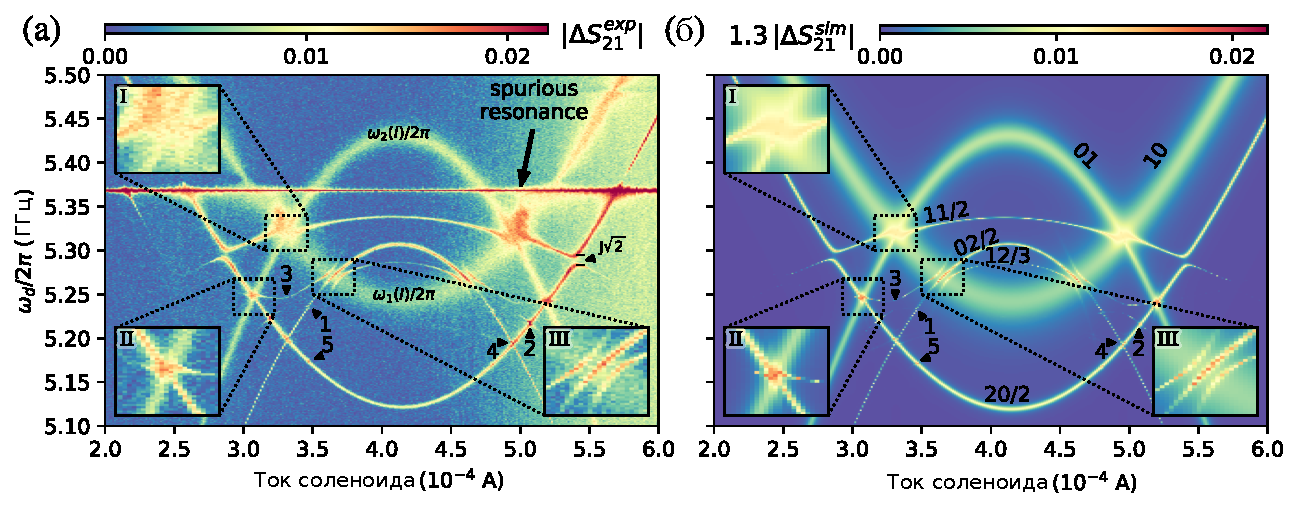
\includegraphics[width=\linewidth]{main_picture}
	
	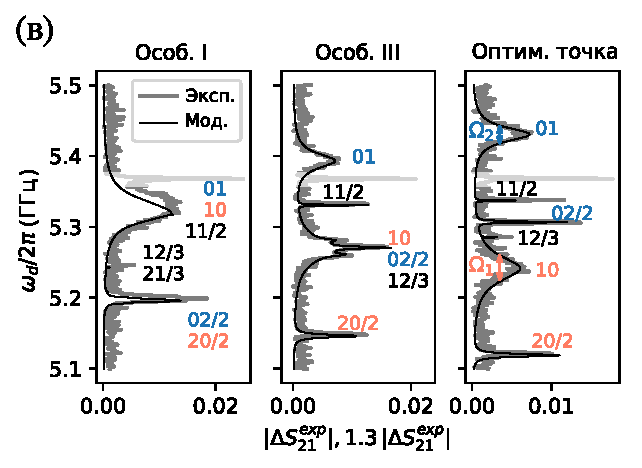
\includegraphics[width=.495\linewidth]{main_picture_slices}
	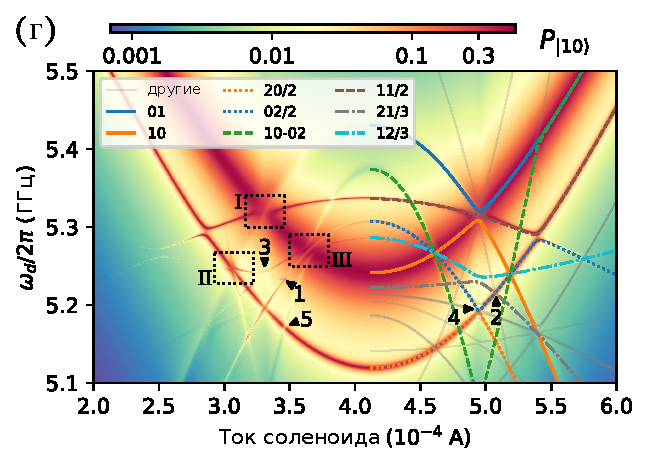
\includegraphics[width=.495\linewidth]{stationary}
	\caption{\textbf{(a)} 
		Данные ДТС. Цветом показан модуль отклонения $|\Delta S^{exp}_{21}| (I, \omega_d)$ комплексного коэффициента пропускания от значения в левом нижнем углу графика. 
		Трансмоны выровнены как на 
		\autoref{fig:experiment2}~(в) и их спектральные линии формируют симметричную картину. Данные содержат дополнительную горизонтальную линию, вызванную взаимодействием резонатора с некоей паразитной модой. Три эффект, не предсказываемые невозмущенной моделью, показаны во вставках I, II и III; остальные особенности, воспроизводящиеся полной численной моделью, пронумерованы арабскими цифрами (см. описание в тексте). \textbf{(б)} Результаты численного расчета (см. обозначения в тексте). Рассчитанное значение $|\Delta S^{sim}_{21}| (I, \omega_d)$ искусственно увеличено в 1.3 раза для достижения количественного совпадения с экспериментом.
		\textbf{(в)} Срезы (а) and (б) при нескольких значениях тока соленоида: 0.333 мA (особенность I), 0.365 мA (особенность III), 0.411 мA 
		(оптимальная точка); 
		экспериментальные данные показаны серым, счет черным цветом. Значения $\Omega_{1,2}/2\pi$ могут быть получены из  
		ПШПВ спектральных линий 10 и 01, 
		соответственно. \textbf{(г)} Рассчитанная заселенность  
		уровня $\ket{10}$ в зависимости от $I$ and $\omega_d$. Кривыми показаны частоты разнообразных переходов, вычисленные из невозмущенного гамильтониана. На легенде подписаны основные переходы в таком порядке, как они расположены в окрестности оптимальной точки; если линии затем проходят через квазипересечение, подписи должны быть переставлены. Под отметкой ``другие'' мы помещаем все остальные переходы системы (одно- и многофотонные), попадающие в диапазон частот графика.}
	\label{fig:two-tone}
\end{figure}


Чтобы проверить, может ли стандартная теоретическая модель воспроизвести особенности спектра, автором численно решалось уравнение \eqref{eq:master} и находились установившиеся состояния системы $\hat \rho_{ss}(I, \omega_d)$, а вместе с ними и соответствующие результаты измерения $\Tr[\hat M \hat \rho_{ss}(I, \omega_d)]$. Итоги такого моделирования представлены на \autoref{fig:two-tone} (б) и, как видно, в действительности хорошо воспроизводят все спектральные особенности эксперимента при использовании всего 9 базисных состояний. Уравнение \eqref{eq:master} решалось как во вращающейся системе в ПВВ при помощи \eqref{eq:steady}, так и в лабораторной системе с расчетом пропагатора за период согласно \eqref{eq:propagator}, но никаких заметных отличий в результатах не было обнаружено; моделирование вторым способом без ПВВ, однако, занимало для массива 401$\times$401 значений токов и частот около 9 часов, в то время как для того же расчета в ПВВ требовалось около 3 минут. Фиксированными параметрами являлись $\Omega_{1,2}$ (равные 20 и 10 МГц, соответственно) и константы невозмущенного гамильтониана, определенные путем аппроксимации экспериментальных спектральных линий кривыми, полученными при численной диагонализации невозмущенного гамильтониана. Константа взаимодействия $J$ обычно определяется в таком методе по квазипересечению между $\omega_1$ и $\omega_2$. Так как на \autoref{fig:two-tone} (а) оно оказывается скрыто из-за большой интенсивности возмущения, проводилось отдельное измерение на меньшей мощности, откуда было получено значение $J/2\pi = 8.69$ МГц. Силу связи можно иначе определить путем наблюдения квазипересечения, расположенного на частоте 5.3 ГГц при токе 0.29 мА (или 0.54 мА). Оно образовано хорошо изученным эффектом \cite{dicarlo2009demonstration}, широко используемом для реализации двухкубитных операций типа cPhase на трансмонах; его величина составляет $(2\times J_\text{eff})/2$, где $J_\text{eff} = \sqrt 2 J$ определяется соответствующим матричным элементом $\hat H_\text{int}$, а деление пополам необходимо, так как в эксперименте наблюдаются двухфотонные процессы. Хорошее соответствие между экспериментальными данными и расчетом можно видеть также из срезов, изображенных на \autoref{fig:two-tone} (в) (паразитный резонанс смягчен цветом).

Также при моделировании дисперсионного оператора измерения было обнаружено, что в эксперименте при возбуждении СИМ провал резонатора не только сдвигался, но и несколько уменьшался по глубине. Это приводило к увеличенной величине отклика по сравнению с чистым моделированием путем сдвига резонансной кривой, поэтому для графиков \autoref{fig:two-tone} (б,в) пришлось на 30\% увеличить все значения данных для достижения совпадения с экспериментом. Автор считает, что данная проблема каким-то образом связана и с аномально малым значением внутренней добротности этого резонатора, которая оказалась в 100 раз меньшей, чем у тестовых резонаторов на том же чипе. Автор наблюдал такое уменьшение внутренней добротности в резонаторах, соединенных с кубитами, на нескольких устройствах, поэтому, если она связана с кубитами, можно предположить и то, что она может оказаться чувствительной к их состоянию. Однако, эта проблема не является критичной для текущего исследования, так как не затрагивает поведения самой СИМ.

Возвращаясь к спектральным данным, мы отмечаем, что особенности I, II, III, показанные во вставках, не могут быть объяснены используя только невозмущенный гамильтониан, который использовался при составлении полной модели \eqref{eq:master}; это можно легко видеть по спектральным линиям, получаемым при его численной диагонализации. Они изображены на \autoref{fig:two-tone} (д), где мы строим все возможные одно- и многофотонные переходы, попадающие по частоте в экспериментальный диапазон (см. пояснения ниже). Как видно, несмотря на то, что, например, квазипересечение, отмеченное как особенность 3, воспроизводится ею правильно, невозмущенная модель не предсказывает никаких переходов, следующих за спектральными линиями в областях, отмеченных римскими цифрами.

До сих пор мы установили лишь то, что одна и та же модель для СИМ дает разные спектры в зависимости от того, учитывается ли внешнее возмущение, и что экспериментальные данные хорошо согласуются с расчетом, использующим полную модель. Для того, чтобы понять природу спектральных особенностей I, II, III, мы описываем более подробно данные на \autoref{fig:two-tone} в следующем разделе.

\section{Анализ спектров}

\subsection{Идентификация переходов}

Хотя невозможно описать все спектральные явления эксперимента невозмущенной моделью, она, тем не менее, служит хорошей отправной точкой для анализа, так как позволяет определить природу спектральных линий вдали от областей с необъясненными особенностями. Итак, на \autoref{fig:two-tone} (д) изображены частоты переходов $\omega_{mk}/2\pi = (E_k - E_m)/h$, где $k>m$; $k,m = 0,1,2,...8$ (если речь идет об $n$-фотонном процессе, частота дополнительно делится на $n$). Так как число состояний СИМ невелико, можно быстро установить соответствие между спектральными линиями и кривыми $\omega_{mk}/n$. Так как в оптимальной точке состояния СИМ практически факторизованы, для спектральных линий мы вводим там обозначения $ij/n$, где $i,j$ определены так же, как и ранее. Те же обозначения для удобства присутствуют и на \autoref{fig:two-tone} (б, в). Если при отходе от оптимальной точки две линии проходят через квазипересечение, то их обозначения затем надо будет поменять местами с другой его стороны. Внутри квазипересечений выбранные обозначения смысла не имеют, так как собственные состояния не являются там факторизованными, однако позволяют определить, что это за суперпозиции.

Перейдем к перечислению многофотонных переходов, образующих все линии, кроме двух однофотонных 01 и 10 ($\omega_{1}$ и $\omega_{2}$). Линии 02/2 и 20/2 очень легко обнаруживаются в трансмонах и лежат параллельно основным линиям на расстоянии $|\alpha_{1,2}/2|$. Другой двухфотонный процесс $11/2$ соответствует одновременному возбуждению двух трансмонов (он, как раз, используется для операции bSWAP, о которой говорилось ранее во введении \cite{poletto2012entanglement}); в нашей работе он участвует в образовании особенности I. Трехфотонный процесс $12/3$ хорошо различим ниже линии $02/2$. Как мы увидим, процессы $12/3$ и $21/3$ будут играть ключевую роль в образовании особенностей III и II, соответственно. Следует отметить, что переходы $11/2$, 21/3, и 12/3 запрещены без взаимодействия между трансмонами ($J=0$), а, значит, являются исключительно свойством СИМ как целого.

Скажем также несколько слов о квазипересечениях, которые предсказываются невозмущенной моделью. В первую очередь они возникают, конечно, между переходами 01 и 10, затем между 11 и 02 (20), которые уже обсуждались ранее. Также интересно квазипересечение под номером 3, образованное трехфотонными процессами в той же точке по току, где пересекаются 10 и 01.

\subsection{Анализ особенностей I, II, III}

Первым шагом к пониманию природы данных особенностей было воспроизведение особенности III в дополнительном численном эксперименте с сокращенным базисом состояний, где для трансмона 1 было учтено два уровня, а не три. После этого стало понятно, что особенности II и III имеют одну и ту же природу и различаются лишь перестановкой трансмонов.

Из \autoref{fig:two-tone} (г) мы заключаем, что наблюдаемое квазипересечение в области III образовано переходами 12/3 и $ 10-02 $ (однофотонный $\ket{10}\rightarrow\ket{02}$), которые оказываются в резонансе при $\omega_1 = \omega_2 + \alpha_2/2$. Последний обнаруживает себя через расселение уровня 10, и поэтому гораздо лучше различим на \autoref{fig:two-tone} (г), чем на (а, б). Аналогичная картина возникает и для особенности II: 21/3 пересекает $ 01-20 $ когда $\omega_2 = \omega_1 + \alpha_1/2$. Проводя дополнительные измерения и численные расчеты, мы далее обнаруживаем, что расщепление зависит от мощности излучения; результаты представлены на \autoref{fig:zoom}

\begin{figure}
	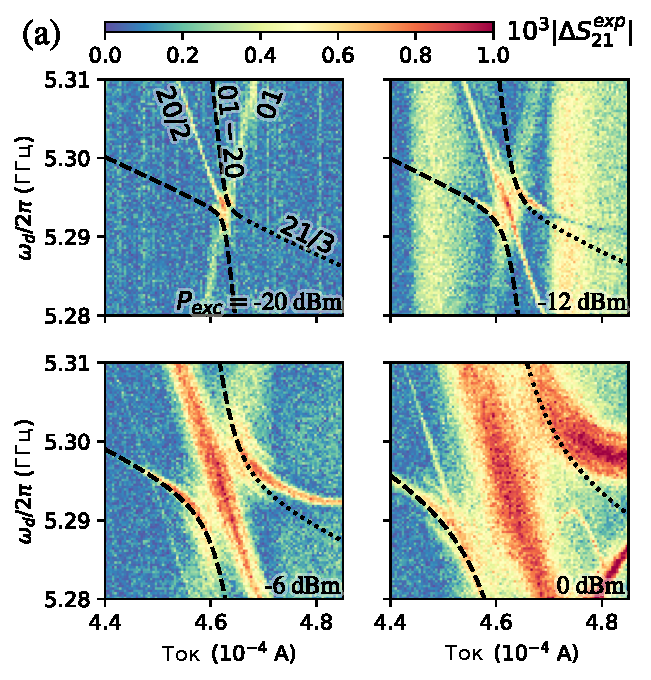
\includegraphics[width=.49\linewidth]{powerscan}
	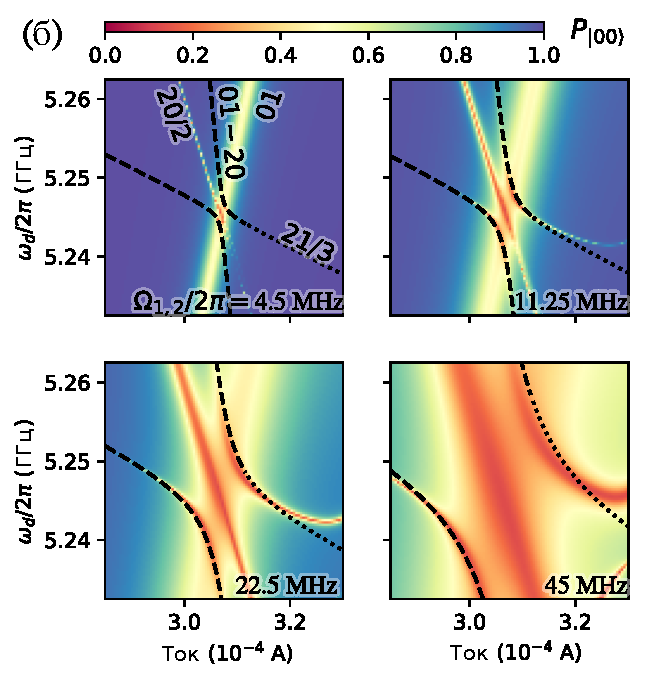
\includegraphics[width=.49\linewidth]{zoom2_picture}
	
	\centering
	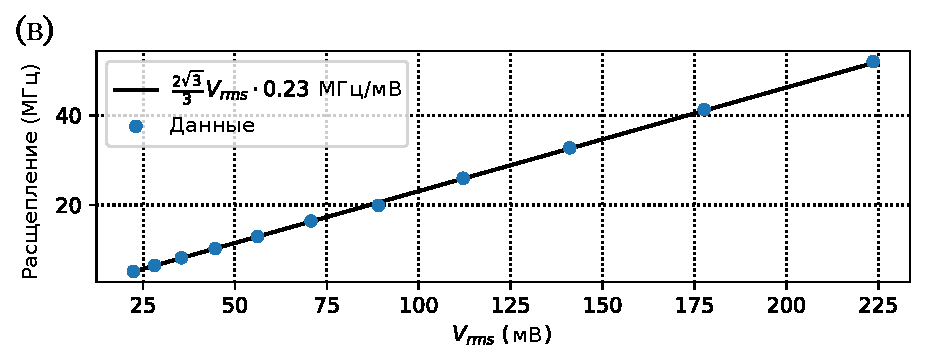
\includegraphics[width=.7\linewidth]{powerscan_1d}
	\caption{Power dependence of feature II: 
		experiment, simulation and analytical model. Dashed are the model curves turning to dotted when the 
		model is not expected to be valid (see text); model values for 
		$\Omega_{1,2}$ are the same for both (a) and 
		(b): $\Omega_{1,2}/2\pi=$ 4.5, 11.25, 22.5 
		and 45 MHz. \textbf{(a)} Experiment (second 
		cooldown; the system parameters are slightly different to 
		those in \autoref{fig:experiment}). The power 
		of the microwave source is increased from -20 
		to 0 dBm, and the corresponding growth of the 
		splitting and the widths of the spectral 
		lines is observed. \textbf{(b)} Simulation 
		with amplitudes of the driving $\Omega_{1,2}$ 
		equal to the model values; other parameters 
		as in \autoref{fig:two-tone}. Note that now 
		colors show the steady-state population of the ground 
		state. \textbf{(c)} Linear dependence of the 
		splitting size on the driving voltage of the 
		microwave source $V_{rms}$, ${\Omega_2}/{V_{rms}} = 2 \pi\cdot 0.23\ 
		{\text{MHz}}/{\text{mV}}$. From Section , the splitting size is 
		$\frac{2\sqrt{3}}{3} \Omega_2$.}
	\label{fig:zoom}
\end{figure}

\chapter{Фотонный транспорт сквозь одномерную цепочку Бозе-Хаббарда}

\chapter{Заключение}



\appendix
\renewcommand*\thesection{\Alph{chapter}.\arabic{section}}

\chapter{Метод максимального правдоподобия}\label{sec:MLE}

Для вектора $ \mathbf{w} $ параметров модели рассчитаем условную вероятность (функцию правдоподобия) $\mathcal{L}(\mathbf{p}|\mathbf{w})$ обнаружить выборку из $ N $ точек $\mathbf{p} = \{x_i, y_i\}_{i=1}^N$ если считается, что они независимы и распределены по нормальному закону вокруг модели ($\mathbb{N}_{\mu_i, \sigma}$, $\mu_i = \mathcal{M}(x_i, \mathbf{w}),\ \sigma = \text{const}$). Искомое выражение будет произведением плотностей вероятности обнаружить каждую точку в соответствующем месте:
\begin{equation}
\mathcal{L}(\mathbf{p}|\mathbf{w}) = \prod_{i=1}^{N} \frac{1}{\sqrt{2\pi}\sigma} \exp[ -(f_{r,i} - \mu_i)^2 / 2 \sigma^2].\label{eq:MLE} 
\end{equation}
Метод максимального правдоподобия (ММП) состоит в нахождении оптимального вектора параметров, доставляющего максимум $\mathcal{L}$. Будем называть этот вектор $ \mathbf{w}^*$, являющийся случайной величиной, зависящей от выборки $\mathbf{p}$, оценкой истинного вектора параметров $\mathbf{w}^0$. Если рассчитать отрицательный логарифм от функции правдоподобия, можно получить отрицательную логарифмическую функцию правдоподобия:
\begin{align*}
- \ln \mathcal{L}(\mathbf{p}|\mathbf{w}) &= \sum_{i=1}^N (f_{r,i} - \mu_i)^2 / 2 \sigma^2 + N \ln\sqrt{2\pi}\sigma
\label{eq:logL} \\
&\equiv \chi^2/2 + N\ln \sqrt{2\pi}\sigma,
\end{align*}
для которой задача превращается в нахождение минимума. В силу независимости второго слагаемого данного выражения от вектора параметров, задача сводится к минимизации суммы квадратов, или $\chi^2$.

Далее, обсудим дисперсию ММП-оценки $\mathbf{w}^*$. Если пренебречь её смещенностью (вообще, для нелинейной задачи ММП, т.е., когда модель нелинейно зависит от параметров, смещение всегда присутствует, но может быть вычислено лишь приближенно и падает как $1/N$ с ростом размера выборки \cite{cox1968}) можно воспользоваться многомерным неравенством Рао-Крамера для ограничения дисперсии снизу. В общем виде оно записывается следующим образом \cite{keener2011, schervish2012}:
\begin{equation}
\text{Var}_\mathbf{w}[\mathbf{w}^*] \geq \text{diag} [\hat I(\mathbf{w})^{-1}],\ \forall\,\mathbf{w}.
\label{eq:cramer-rao}
\end{equation} 
Здесь $\mathbf{w}$ обозначает какой-то произвольный вектор параметров, считающийся истинным, $\hat I(\mathbf{w})$ -- информационная матрица Фишера. Разумеется, значение элементов матрицы Фишера зависит от $\mathbf{w}$: при нелинейном ММП для некоторых значений вектора параметров функция правдоподобия может меняться очень быстро, а для других, наоборот, быть практически плоской. В эксперименте невозможно узнать, в какой же именно точке $\mathbf{w} =\mathbf{w}^0$ находятся истинные параметры распределения, генерирующего данные, чтобы рассчитать там матрицу Фишера. Поэтому для получения оценки берется параметр $\mathbf{w}  = \mathbf{w}^*$ в надежде, что матрица Фишера окажется там примерно такой же, как и в истинной точке. Используя определение $\hat I(\mathbf{w})$, свойства $\ln \mathcal {L}$ и предполагая, где необходимо, двойную дифференцируемость, получим \cite{keener2011, schervish2012}:
\begin{align*}
\hat I(\mathbf{w}) 
&= E_\mathbf{w} \left[ \nabla_\mathbf{w} \ln \mathcal{L} \cdot \nabla_\mathbf{w}^T \ln \mathcal{L} \right]\\
&= E_\mathbf{w} \left[ - \mathbb{H}_\mathbf{w} \ln \mathcal{L} \right],
\end{align*}
где $E_\mathbf{w}$ означает матожидание по функции правдоподобия, т.е. среднее по возможным реализациям выборки $\mathbf{p}$, распределенной согласно \eqref{eq:MLE}, а 
\[
\mathbb{H}_\mathbf{w} = 
\left(\begin{matrix}
\partial^2/\partial w_1^2 & \partial^2/\partial w_1 \partial w_2 & \dots \\
\partial^2/\partial w_1 \partial w_2
& \partial^2/\partial w_2^2 & \dots\\
\vdots & \vdots & \ddots
\end{matrix}\right).
\]
Используя \eqref{eq:MLE} и тот факт, что $E_\mathbf{w}[y_i] = \mu_i (x_i, \mathbf{w})$, можно получить аналитическое выражение для $\hat I(\mathbf w)$:
\begin{equation}
\hat I(\mathbf{w}) = \sum_i \frac{\mathbb{H}_\mathbf{w} \mu_i^2(x_i, \mathbf{w}) - 2 \mu_i(x_i, \mathbf{w}) \mathbb{H}_\mathbf{w} \mu_i(x_i, \mathbf{w})}{2\sigma^2}.
\label{eq:fisher_analytic}
\end{equation}
Эта формула верна для любой задачи ММП с гауссовским шумом и может применяться для быстрых расчетов без необходимости вычисления численного градиента. Таким образом, для получения информационной матрицы требуется, во-первых, вычислить гессиан модельной функции $\mathcal{M}(x, \mathbf{w})$ в точке $\mathbf{w} = \mathbf{w}^0$ (или $ \mathbf{w}^0 $, если данные синтетические); во-вторых, необходимо выяснить величину $\sigma$. Для этого часто применяется метод оценки дисперсии по выборке $\{y_i - \mu_i\}$, однако здесь следует учитывать тот факт, что при нелинейном МПП невозможно получить аналитическое выражение для соответствующей оценки $ (\sigma^2)^* $ из-за неопределимого эффективного числа степеней свободы \cite{ye1998, andrae2010}. В эксперименте можно решить эту проблему находя $\sigma$ независимо, многократно повторяя измерения в одной точке. Другим способом является применение формулы, верной лишь для линейной регрессии $(\sigma^{2})^* = \chi^2/(N-M)$, где $M = \dim \mathbf{w}$, и затем проверить её точность при помощи метода Монте-Карло. В контексте аппроксимации моделей однотоновых спектроскопий автором проводились тесты с 5000 запусками, которые в частности показывали, что при $M=6$ и $N=18$ $ (\sigma^{2})^* $ согласуется с известной $\sigma^2$ для синтетических данных с точностью 1\% ($|E[(\sigma^{2})^*] - \sigma^2|< 0.01 \sigma^2$). Отсюда делается вывод о возможности использования указанной формулы даже для нелинейного ММП.

В заключение этого раздела приведем еще несколько соображений относительно нелинейного ММП и точности полученных оценок. Понятно, что в силу своего случайного характера при реальном применении ММП компоненты полученного вектора $\mathbf{w}^*$ могут оказаться сколь угодно отличными от истинного значения. Чтобы получить представление о вероятности больших отклонений и, соответственно, понять в какой окрестности  $\mathbf{w}^*$ содержится истинное значение $\mathbf{w}^0$, требуется рассчитать доверительный интервал. Эта величина показывает, что с некоей наперед заданной вероятностью (например, 95\%) значения каждой из компонент $\mathbf{w}^*$ при анализе новых выборок не будут выходить за пределы некоторого интервала (отдельного для каждой компоненты). Расчет доверительного интервала даже для простых распределений достаточно сложен и требует наличия аналитического выражения для функции оценки $\mathbf{w}^*$. При нелинейном ММП такое выражение найти практически невозможно, так как оптимум функции правдоподобия ищется либо путем градиентного спуска, либо состоит в решении системы нелинейных уравнений для поиска экстремумов. При использовании градиентного спуска также возникает зависимость распределения $\mathbf{w}^*$ от распределения векторов начальных условий, хорошо заметная при тестировании по Монте-Карло. Таким образом, нужно с осторожностью относиться к нижней границе дисперсии, вычисленной согласно неравенству Рао-Крамера, так как неизвестно, насколько реальная дисперсия окажется больше. Однако надежду на полезность полученной оценки дает понятие об асимптотической сходимости распределения  $\mathbf{w}^*$ к нормальному при увеличении размера выборки до бесконечности \cite{jennrich1969, anastasiou2017}. В таком случае вычисление гессиана в оптимальной точке даст ковариационную матрицу для вектора параметров и позволит вычислить доверительную область. Таким образом, можно ожидать хорошей точности ММП при избыточности данных, если градиентный метод не вносит больших ошибок, связанных с зависимостью от начальных условий оптимизации.
 

\renewcommand\bibname{Список литературы}
\bibliographystyle{ugost2008}
\bibliography{dissertation.bib}
\end{document}
